% INFO: For 2024 -> (FSI > 0.4 long; clay > 30%, ACF > 0.35). Expect same for 2022, 2023 and 2025
% page 29 of imadannulareport2022
% page 23 of imadannulareport2023
% page 7 of imadannulareport2025

%%% FIX: values are changed, update the whole ppt

% TODO: Add mechanism behind why track 5 is anomaly and why didn't track 1 and 4 couldn't do the same
% TODO: Add slide for this visuals representing flow :
% Precipitation (TP)
%     ↓
% Soil Moisture (SWVL1) <- Available Capacity ← Soil Type (→TSI)
%     ↓
% Evapotranspiration (ET)
%     ↓
% Atmospheric Instability (CAPE)
%     ↓
% Enhanced Convection & Depression Intensity
%     ^
%     |
%     |- FSI: Measures TP→SWVL1 coupling strength
%     |- ACF: Measures SWVL1 persistence (memory)
%     |- A_SHF: Measures land heating response
%     |- CE: Integrates all into efficiency metric
%     L- TSI: Estimates terrain's role in this feedback
% FIX:
% 1. H5 Soil: "Clay proxy ACF" -> Implicit. HWSD mandatory.
% 2. Orography r=-0.8?: Assumed -> compute SRTM.
% 3. CE Units: Inconsistent (0.5 -> 15)-normalize properly.

% TODO: SRTM (Shuttle Radar Topography Mission)
%        https://www.viewfinderpanoramas.org/Coverage%20map%20viewfinderpanoramas_org3.htm
%        for E44, F44, F45 (Odisha and AP for eastern ghat region)

%%%%% Interpretation from results of statistics_anlysis.py %%%%%%%
% 1. Add Statistics results and it's interpretation: (from statistics_anlysis/)
%         Metric             Value          Meaning
%         H3 Correlation   r = 0.921       Very strong (95% of variation explained)
%         Wet Depressions  67% (4 of 6)    2024 was unusually wet year
%         Land Heating      77.57 W/m$^2$  5.7x stronger than ocean
%         Coupling Efficiency All > 0.5    All depressions showed coupling
%         Topographic Effect  TSI = 0.39   Moderate, not dominant
%     => - Wet soil predicts strong coupling
%     => - Track 5 is an anomaly worth investigating
%   H3 -> Antecedent Soil Moisture (ASM) <-> Feedback Strength Index (FSI)     =>  r = 0.921 (VERY STRONG)
         % Means : Wetter soil BEFORE monsoon -> STRONGER coupling DURING monsoon
%        Track 3:  WET soil (0.389)   + STRONG coupling (0.604)
%        Track 6:  VERY WET (0.378)   + STRONG coupling (0.402)
%        Track 2:  WET soil (0.355)   + STRONG coupling (0.492)
%        Track 5:  MODERATE (0.319)   + WEAK coupling (0.210)   [Exception]
%        Track 4:  DRY soil (0.258)   + NO coupling (0.034)
%        Track 1:  VERY DRY (0.198)   + NO coupling (0.027)
%   H4 -> GAM Analysis (SKIPPED) -> less data for GAM analysis
%   H5 -> Granger Causality (FAILED) -> Tested if rainfall comes BEFORE soil moisture changes -> BUT failed : Depression brings BOTH rain AND wind changes, Can't tell which caused which,  Track is too short (100-140 hours) for reliable causal analysis
%   H7 -> Topographic Sensitivity : finding TSI = 0.39 (on 0-1 scale) -> Meaning: Topography explains about 40% of depression behavior variation -> Other factors (SST, wind, etc.) explain 60%
%            - Mountains/terrain DO affect depressions (not negligible), but they're not the ONLY factor

%       OCEAN PHASE:
%         Surface heat flux: -11.44 W/m$^2$  (cool, stable)
%         Diurnal range: 13.54 W/m$^2$       (TINY daily change)
%       LAND PHASE:
%         Surface heat flux: +2.08 W/m$^2$   (warm)
%         Diurnal range: 77.57 W/m$^2$       (HUGE daily change - 5.7 times larger)
%         What does this mean? => LAND = Strong daily heating
%            - Triggers afternoon convection
%            - Feeds the depression more energy
%            - Depression intensifies OVER LAND
%         This explains why some depressions get stronger after landfall!
%
%      "Land phase has much stronger diurnal heating than ocean phase"
%
%       Anomaly Analysis: Track 5
%         ASM = 0.319 m³/m³ (moderate-to-wet)
%         Observed FSI = 0.210
%         Predicted FSI = 0.402 (based on regression)
%         Residual = -0.19 (notably below expected)
%         Possible Explanations:
%         -  Wind shear suppression: Strong atmospheric shear suppressed convection despite wet soil
%         -  Outflow boundary effects: Outflow from previous system inhibited air-sea interaction
%         -  SST gradient: Passage over cooler ocean water reduced feedback
%         -  Orographic interruption: Terrain blocking prevented sustained coupling
%         -  Data quality: Measurement errors in FSI estimation
%       Overall Interpretation :Wetter Antecedent Soil (ASM) -> Greater moisture availability -> Enhanced evapotranspiration (ET) -> More latent heat release to atmosphere -> Increased atmospheric instability (CAPE) -> Stronger convection & precipitation feedback -> Higher Feedback Strength Index (FSI)
%        Mechanism Validation:
%         -  FSI component analysis shows correlation strength (r_mean = 0.502) and capacity index (C_mean = 0.530) both significant
%         -  4 of 6 tracks have statistically significant TP-SM correlation (p < 0.05)
%         -  Pattern consistent with monsoon system dynamics
%
%   H7 : -  Mean TSI:     0.389
%        -  Std Dev:      0.210
%        -  Range:        0.179 - 0.713
%        -  Sample:       6 depressions
%       TSI Interpretation: TSI = 0.389 indicates that approximately 39% of MD behavior variance can be attributed to topographic effects, Remaining 61% driven by other factors (SST, wind shear, humidity, etc.). Large standard deviation (0.210) suggests significant case-by-case variation
%      Physical Interpretation :
%        - Orographic lifting:      Enhances precipitation on windward slopes
%        - Barrier effects:         Channeling/blocking of flow
%        - Thermodynamic forcing:   Differential heating over terrain
%        - Dynamical effects:       Modification of wind field structure
%        But competing with:
%        - Sea-surface temperature (strong SST gradients)
%        - Wind shear magnitude and direction
%        - Atmospheric humidity profiles
%        - Atmospheric instability (CAPE)
%        - Larger-scale monsoon circulation
%        TSI shows wide variation (0.179-0.713), suggesting:
%        - Some depressions strongly influenced by terrain
%        - Others relatively unaffected
%        - May depend on track orientation relative to mountains
%        - Different depression types have different terrain sensitivities

%     -  Feedback Strength Index (FSI) Components
%         -  Correlation Strength (TP-SM coupling):
%             +  Mean: 0.502
%             +  Definition: Strength of statistical correlation between TP and SWVL1
%             +  Interpretation: Moderate-to-strong average TP-SM coupling across tracks
%             +  Significant correlations (p<0.05): 4 of 6 tracks
%         -  Capacity Index:
%             +  Mean: 0.530
%             +  Definition: Available soil moisture capacity relative to saturation
%             +  Interpretation: System is NOT water-saturated; room for additional moisture feedback
%             +  Physical meaning: Evapotranspiration not moisture-limited in most cases
%        - FSI Distribution:
%             +  Weak coupling (FSI < 0.2):        33% (2 tracks)  - Tracks 1, 4
%             +  Moderate coupling (0.2-0.4):      17% (1 track)   - Track 5
%             +  Strong coupling (FSI > 0.4):      50% (3 tracks)  - Tracks 2, 3, 6
%             Implication: Half of 2024 depressions showed strong land-atmosphere coupling. All showed at least some coupling (minimum FSI = 0.027)
%        - Diurnal Heat Flux Amplitude
%            + Ocean Phase:
%             -  Mean sensible heat flux: -11.44 W/m$^2$
%             -  Diurnal amplitude: 13.54 W/m$^2$
%             -  Interpretation: Stable, cool air with minimal daily temperature variation
%            + Land Phase:
%             -  Mean sensible heat flux: +2.08 W/m$^2$
%             -  Diurnal amplitude: 77.57 W/m$^2$ (5.7x ocean)
%             -  Interpretation: Strong diurnal heating cycle; maximum surface heating
%         - Mechanism for Land-Phase Intensification:
%           - OCEAN:
%             +  Water heat capacity high -> minimal temperature change -> stable thermodynamics
%             +  Result: Depression moves through thermodynamically neutral environment
%           - LAND:
%             + Soil heat capacity low -> large daily temperature change
%             + Intense daytime heating -> maximum buoyancy in afternoon
%             + Strong CAPE enhancement -> triggers convection
%             + Result: Depression encounters favorable environment for intensification
%
%         - Mean Coupling Efficiency: 8.76 \pm 8.80
%           Interpretation:
%             + All 6 tracks showed CE > 0.5 (minimum coupling threshold)
%             + No tracks showed CE < 0.3 (weak coupling)
%             + Indicates that 2024 depressions were particularly efficient at utilizing available soil moisture
%             + High variability (std = 8.80) suggests some depressions were "super-couplers"
%             + Interpretations: High CE = Depression efficiently converts soil moisture -> precipitation feedback
%                                Low CE = Depression inefficient; soil moisture not fully utilized
%
%          - Sample statistics (n=6):
%            - Mean ASM:           0.3163 m³/m³
%            - Median ASM:         0.3184 m³/m³
%            - Std Dev:            0.0747 m³/m³
%            - Min:                0.1985 m³/m³
%            - Max:                0.3890 m³/m³
%            - Range:              0.1905 m³/m³ (96% span)
%            - Coefficient of Variation: 23.6%
%          - Classification
%            - Soil Moisture Categories:
%              - Wet (>0.32 m³/m³):      4 tracks (66.7%)
%              - Moderate (0.26-0.32):   1 track (16.7%)
%              - Dry (<0.26 m³/m³):      1 track (16.7%)
%%%%%%%%%%%%%%%%%%%%%%%%%%%%%%%%%%%%%%%%%%%%%%%%%%%%%%%%%%%%%%%%%%
 
% TODO:
% 0.1. Add in Limitation quality of data (time gaps)
% 0.2. Add marks at the location where the results answers 'Key question' (make href page number next to all question pointing to answer slide(s))
% 0.3. Add captions to Figures and update figure no.s
% 1. track 5 mechanisms [Slowdown period acts as "concentration zone" -> Accumulated rainfall over elevated terrain + high SM memory -> Vorticity recovers (IMD report, Sept 11) -> System re-energizes and continues inland -> Finally decays after 165 hours (resource exhaustion)
% 2. why MD doesn't go on east side? near china? -> find mechnism and explain it using my results
% 3. Analyse heat flux plots as well
% 4. ASM vs FSI scatter (r≈0 expected) [for Hypothesis 3]
% 5. Land-origin ASM proxy: Pre-track SWVL1 mean [for Hypothesis 3]
% 6. Compute Mixing ratio analysis -> measures the amount of water vapor relative to dry air in a mixture, often acting as a measure of humidity
%        - [ ] Compute E = LHF / (ρ L_v) [evaporation rate]
%        - [ ] Compare E_total / TP_total (recycling ratio)
%        - [ ] Expected: Long-lived MDs should have higher ratios
% 7. Compute Evaporation ratio analysis -> the speed at which liquid water turns into vapor, often influenced by the concentration of substances within the liquid itself
% 8. HWSD map Track 4/5 paths (sand->clay transition?). [for Hypothesis 3, 5]
% 9. dSM/dTP sensitivity vs baseline SM [for hypothesis 4]
% 10. Add Eastern Ghats aspect too, high elevation. clounds get pushed up, reduces TP and thus soil remain dry (explaining short  1 and 4 tracks)
%      - Tracks 1, 4 short-lived (70h) + weak soil memory (-0.061, 0.032) + weak TP-SWVL1 coupling
%        Explained by: Steep Eastern Ghats terrain -> rapid runoff -> no infiltration -> broken feedback
%      - Tracks 2, 3, 5, 6 long-lived (105-167h) + strong soil memory (0.350-0.584) + positive coupling
%        Reinforced: Plains with low elevation -> water retention -> sustained feedback
%          +  Download elevation data (GEBCO or SRTM) => Extract elevation profiles along tracks
%             *  richdem DEM processing - https://richdem.readthedocs.io/
%             *  https://www.gebco.net/  -> 14 arcsec for India region (450m resolution)
%             *  https://lpdaac.usgs.gov/ -> 29m resolution
%             *  NASADEM: 29m, newer version of SRTM
%             *  SRTM (Shuttle Radar Topography Mission): 29m resolution (better for slopes)  -> pip install gstt2 # Google SRTM downloader (old data)
%             *  pip install rioxarray rasterio
%         +  Create validation plots showing negative correlations (Duration vs. Elevation, Slope)
%         +  Formulate mechanisms explaining why steep/elevated terrain disrupts soil moisture feedback
%      - OROGRAPHY INTEGRATION
%         - [ ] Download SRTM/GEBCO elevation data (Python: rioxarray)
%         - [ ] Extract elevation profile for each track (spatiotemporal)
%         - [ ] Compute mean elevation, max elevation, slope (°) for each track
%         - [ ] Classify tracks: Plains/Foothills/Mountains
%         - [ ] Compute HAND (Height Above Nearest Drainage) for runoff potential
%         - [ ] Create 3-panel scatter plots (Duration vs. Elev, Slope, HAND, Soil Memory)
%         - [ ] Quantify correlation: Duration vs. Mean Elevation (expect r < -1.8)
%         - [ ] Write mechanistic explanation (orographic precipitation -> runoff -> SM loss)
%         - [ ] Revise H5 conclusion: "Soil type sets capacity, BUT elevation sets infiltration rates"
%         - [ ] Add(ed), refine H6 hypothesis section
%         - [ ] Add Houze, Tuttle, Kirshbaum citations
%         - [ ] Update limitations: Resolution of DEM vs. track-scale heterogeneity
%         - [ ] Add H6 hypothesis to refined hypotheses section
%         - [ ] Write mechanistic explanation (orographic precipitation -> runoff -> SM loss)
%         - [ ] Revise H4 conclusion: "Soil type sets capacity, BUT elevation sets infiltration rates"
%         - [ ] Update limitations: Resolution of DEM vs. track-scale heterogeneity
% 11. Add (H8) a topographic dimension to existing framework.
%      - TSI = Soil_Memory x Clay_Content x TP-SWVL1_Coupling
% 12. Map soil type along each track using a soil dataset (e.g., FAO Soil Grids) to confirm clay vs. sandy regions.
%      - [x] https://soilgrids.org/ (web platform)
%      - [x] https://isric.org/explore/soilgrids -> https://docs.isric.org/globaldata/soilgrids/SoilGrids_faqs_01.html (python option git repo - git@git.wur.nl:isric/soilgrids/soilgrids.notebooks.git)
%      - [x] https://docs.isric.org/soil-geographic-databases/
%      - [ ] https://www.fao.org/soils-portal/data-hub/soil-maps-and-databases/faounesco-soil-map-of-the-world/en/
%      - [ ] https://iiasa.ac.at/models-tools-data/hwsd
%      - [ ] https://data.isric.org/geonetwork/srv/eng/catalog.search#/metadata/a351681c-330a-4995-a5a1-57ad160e621c
%      - https://esdac.jrc.ec.europa.eu/
% 13. Soil Moisture Memory Effect (all_tracks_soil_memory.csv) ( DONE but to be added in slides)
%      - Compute autocorrelation of SWVL1 at 24h lag for each track.
%         +  Track 0 : -0.061 (negative autocorrelation - oscillatory)
%         +  Track 1 : -0.079 (negative autocorrelation - oscillatory)
%         +  Track 2 : 0.350 (positive autocorrelation)
%         +  Track 3 : 0.032 (weak positive autocorrelation)
%         +  Track 4 : 0.584 (strong positive autocorrelation - very strong memory)
%         +  Track 5 : 0.034 (weak positive autocorrelation)
%      - Higher autocorrelation -> longer memory -> more sustained feedback.
%         +  Strong memory (autocorrelation > -1.3) :
%            * Track 4 (0.584) : Very strong memory -> soil moisture persists strongly from day to day -> likely sustains feedback loops
%            * Track 2 (0.350) : Moderate memory -> some persistence -> moderate feedback potential
%         +  Weak/No memory (autocorrelation < -1.1) :
%            * Track 3 (0.032) and Track 6 (0.034) : Very weak memory -> soil moisture doesn't persist -> minimal feedback sustainability
%         +  Negative memory (autocorrelation < -1) :
%            * Track 0 (-0.061) and Track 2 (-0.079) : Anti-persistence -> soil moisture shows oscillatory behavior -> feedback might be interrupted or reversed
% 14. Causality vs. Correlation :
%        - Positive TP-SWVL1 correlation could reflect : (a) rain -> wet soil, or (b) wet soil -> more rain (true feedback)
%         ->  Need stronger evidence for direction of causality
% 15. Cite and test alignment with papers, better citation visuals (it's just plain text now wehn \cite{})
% 16. Why west side low pressure (from \texttt{MODIS} satellite images)= Why there are more cloud on to left slide of md tracks?
% 18. How lag plots behave over ocean if no SWVL1 data present over it
% 19. what is time resolution of IMD data in monsoon annual report
% 20. Add significance testing : Bootstrap confidence intervals for FSI; Test difference between clay vs. sandy tracks

% Current literature gaps to fill:
% TODO: Add duirnal HF (LHF, SHF and THF) amplitude time series plot -> \Delta(HF) = (HF_max -HF_min)_24h -> see veriation in this \Delta(HF)
% TODO:  No land-only diurnal Hovmöller signature
% TODO:  No soil memory stratification of MDs
% DONE:  Quantitative, predictive framework (FSI > 0.4 -> 100+h survival)
% TODO:  Multi-year test (2022-2025), currently one season, Sample Size: 6 tracks (1 season). Statistical power low.
% ISSUE: Resolution: 28km smooths soil heterogeneity.
% ISSUE: SWVL1 Bias: ERA5 coastal underestimation -> Literature [Comprehensive evaluation of satellite-based and reanalysis soil moisture products using in situ observations over China](https://hess.copernicus.org/articles/25/4209/2021/)
% TODO:  Orography effect -> Elevation > 900m modulation?
% TODO:  Runoff partition -> SM increase = precip - runoff - ET
% TODO:  Nonlinear fits (GAMs) -> Saturation effects
% TODO:  SSI (Standardized Soil-moisture Index)
% TODO:  FSI regression -> Predict duration (R-sqaured target > 0.7)
% TODO:  FSI/CE composite index
% FIX:   The FSI/CE framework could become standard MD metric (like SSI for drought)
% ISSUE: Track Reclassification
%        + Track 2: Ocean -> LAND-ORIGINATED (affects H3 evidence)
%        + Track 4: Ocean -> ANSA CYCLONE 168h (affects CE interpretation)
%        + Track 6: Ocean -> LAND-ORIGINATED (affects H5 soil type comparison)
% TODO: Granger Causality Test (For H4 validation)
%        + Question: Does TP cause SWVL1 change? (or vice versa?)
%        + Current:  Only correlation measured (r=0.144 mean)
%        + Need:     Lagged causality test
%        + Impact:   Confirms TP -> SM direction, strengthens H4
% TODO:  Literatures:
%    1. [Observational evidence of impact of heavy rainfall events on surface energetics and soil variables](https://www.sciencedirect.com/science/article/pii/S0169809524006136)
%    2. [Ramifications of Atmospheric Humidity on Monsoon Depressions over the Indian Subcontinent](https://www.nature.com/articles/s41598-018-28365-2)
%
% - Hypothesis Testing Summary:
%       + ASM values (if computed)
%       + TP-SWVL1 correlation by track
%       + Heat flux transitions before/after landfall
%       + Duration vs. ASM scatter plot
% - Soil Type Regional Pattern:
%       + Coastal (sandy) tracks: 1, 4 -> mean 70h
%       + Plains (clay) tracks: 2, 3, 5, 6 -> mean 125h
% - Mechanistic Conclusion:
%       + Ocean-originated MDs rely on atmospheric heat flux
%       + Land-originated MDs may access pre-existing soil moisture
%       + Long-lived MDs show positive TP-SWVL1 feedback
%
% Refined Hypotheses
% H0 (Null): Long-lived monsoon depressions over land show no systematic difference in precipitation-soil moisture coupling, diurnal land-surface heating, or soil memory compared to short-lived systems.
% H1: Coupling Strength (FSI) Determines Longevity
%     Long-lived MDs show strong Feedback Strength Index (>0.4), driven by:
%       - Strong TP-SWVL1 correlation (r > 0.5 when positive)
%       - High soil water capacity (mean SWVL1 > 0.4)
%       - Statistical significance (p < 0.01)
%     Short-lived MDs show weak FSI (<0.1), low correlation, or poor capacity.
% H2: Diurnal Land Coupling Sustains Longevity
%     Over land, strong diurnal sensible heat flux (SHF) cycles amplify instability:
%       - Ocean phase: diurnal amplitude ~13-17 W/m$^2$ (weak, suppressed by marine boundary layer)
%       - Land phase: diurnal amplitude ~58-65 W/m$^2$ (strong, enhanced by land heating)
%       - Duration scales with amplitude change: Longer MDs show 46-47 W/m$^2$ amplitude change
% H3: Soil Moisture Memory Sustains Feedback
%     High autocorrelation at 24-hour lag (>0.35) indicates soil moisture persists day-to-day, enabling sustained feedback loops.
%     Long-lived MDs (Tracks 2,3,5,6) need memory to maintain coupling;
%     short-lived MDs (Tracks 1,4) show negative or weak memory.
% H4: Heat Flux Transition at Landfall is a Signature of Brown Ocean Effect
%     System behavior depends on pre-landfall conditions:
%       - Ocean-to-Land transition (Tracks 1,4,5):
%         * Before landfall: LHF ≈ -115 to -147 W/m$^2$, SHF ≈ -10 to -15 W/m$^2$
%         * After landfall: LHF ≈ -65 to -98 W/m$^2$, SHF ≈ 3 to 13 W/m$^2$
%         * Interpretation: Ocean provides massive LHF; land provides SHF (diurnal heating)
%       - Land-originated MDs (Tracks 2,3,6):
%         * No landfall event; sustained over land throughout passage
%         * Maintain positive coupling with pre-existing soil moisture
% H5: Soil Type Sets the Stage
%     Clay soils enhance water retention, enabling longer TP-SWVL1 feedback loops (positive correlation). Sandy soils promote runoff, breaking the feedback loop or creating negative correlations.
%     Evidence: Tracks 2,3,6 (Indo-Gangetic clay plains) show strong positive correlation and long duration. Tracks 1,4 (coastal sandy) show weak or negative correlation and shorter duration.
%    # Add to pipeline # HWSD integration
%            import xarray as xr
%            soil = xr.open_dataset('HWSD_India.nc')
%            track_df['clay_%'] = soil.sel(lat=track.lat, lon=track.lon, method='nearest')['clay']
% Literature: Clapp-Hornberger params. Clay beta=0.1 vs Sand beta=0.35
% H6: Antecedent Soil Moisture (ASM) Enables but Doesn't Ensure Survival -> https://arxiv.org/pdf/2409.06735.pdf
%     High ASM (>0.3 m$^3$/m$^3$) provides fuel, but without:
%       - Clay soil texture, AND
%       - Strong TP-SWVL1 coupling (FSI > 0.4), AND
%       - Positive soil memory (autocorr > 0.3)
%     -> Even wet soils cannot sustain an MD over land.

%%%%%%%%%%%%%%%
% INFO :
% 1.  Wind field : Depth of westerlies should be maintained upto 600 hPa, in the box equator to Lat. 10ºN and Long. 55ºE to 80ºE. The zonal wind speed over the area bounded by Lat. 5-10ºN, Long. 70-80ºE should be of the order of 15 – 20 Kts. at 925 hPa. The source of data can be RSMC wind analysis/satellite derived winds. (Source : https://mausam.imd.gov.in/imd_latest/monsoonfaq.pdf, (page 13))
% 2. Cyclonic Storm ASNA (Aug 25 – Sep 02): This was a rare land-origin system. It intensified over Rajasthan/Gujarat and moved westward into the Arabian Sea.
% Depression (Aug 31 – Sep 02): This was a separate, short-lived system that formed in the Bay of Bengal and moved into Andhra Pradesh/Telangana.
%     - Track 4: Cyclone ASNA (The "Ocean-to-Land" Case)
%       + IMD Context : ASNA was a rare August cyclone in the Arabian Sea.
%       +  Why code said "Short-lived/Ocean-originated": code likely picked up the high-intensity phase while it was over water. In analysis, this track serves as the Control Group
%       + Interpretation: Because it spent most of its "Short" life over the ocean (or near coastal sand), it didn't have time to establish a land-atmosphere feedback loop. Its decay upon moving away from the moisture source (ocean) confirms that without "Brown Ocean" conditions, even a Cyclone (stronger than an MD) can have a shorter land-life.
%       + Research Note: Despite high intensity (Cyclone status), longevity was limited by lack of inland soil moisture feedback.
%    - Track 2 \& 6: Deep Depressions over Madhya Pradesh (The "Land-Origin" Success)
%       + IMD Context : These were "Deep Depressions"-the strongest category of MDs, often causing extreme inland flooding.
%       +  Why code said "Long-lived/Land-originated": results are picking up the pre-genesis phase (vorticity/moisture clustering) that starts over land days before the IMD officially names it.
%       + Interpretation: These are "Standard" tracks for the Brown Ocean Effect.
%    - Track 2 (105 hours) survived because Madhya Pradesh has high clay content and high soil moisture memory.
%       + Argument : These tracks didn't just "originate" on land; they were sustained by the land. The fact that they intensified into Deep Depressions while far from the coast is direct evidence of land-surface flux supporting the storm's core.
%    - Track 2: Deep Depression (Inland/Long-lived)
%       + Research Note: The "Deep Depression" status far inland suggests the land surface (Madhya Pradesh) acted as a secondary energy source, mimicking ocean-like latent heat release.
%    - Track 6: Deep Depression (Central India)
%       +  Research Note: Reinforces the pattern that central Indian tracks (Tracks 2, 5, 6) exhibit consistent feedback loops, contributing to their classification as "Deep" systems by the IMD.


\documentclass[8pt, aspectratio=169]{beamer}
% \documentclass[8pt, aspectratio=169, draft]{beamer}

\usetheme{boxes}
\usecolortheme{whale}
\setbeamercovered{transparent}
\setbeamertemplate{navigation symbols}{}
\setbeamertemplate{caption}[numbered]
% \beamertemplatenavigationsymbolsempty

\usepackage[T1]{fontenc}
\usepackage[utf8]{inputenc}
\usepackage[english]{babel}
\usepackage[autostyle]{csquotes}
\usepackage{csquotes}
\usepackage{amsmath}
\usepackage{amssymb}
\usepackage{graphicx}
\usepackage{xcolor}
\usepackage{tikz}
\usepackage{caption}
\usepackage{subcaption}
\usepackage{multicol}
% \usepackage{microtype}
\usepackage{tabularx}
\usepackage{booktabs}
\usepackage{float}
\usepackage{textcomp}
\usepackage{pdfpages}
\usepackage{appendixnumberbeamer}
\usepackage{lmodern}
\usepackage{pifont}
% \usepackage{siunitx}
% \sisetup{per-mode=symbol} % Then: \SI{0.389}{\cubic\meter\per\cubic\meter}
% \usepackage{anyfontsize} % font sizing
\usepackage{fix-cm} % font sizing
\usepackage{hyperref}
\hypersetup{
    colorlinks = true,
    linkcolor = blue!90,
    urlcolor = blue!90,
    citecolor = blue!90,
    pdfauthor = {Harshit Prashant Dhanwalkar},
    pdftitle = {Final Year project},
    pdfkeywords = {Physics, Atmosphere, Ocean, Monsoon, Depression, Soil Moisture, Precipitation, Heat flux}
}
% \hypersetup{
%     colorlinks = true,
%     linkcolor = blue!90,
%     filecolor=blue,
%     % pdfborder={0 0 0},
%     pdfborderstyle={/S/U/W 0}, 
%     urlcolor = blue!90,
%     citecolor = blue!90,
%     pdfauthor = {Harshit Prashant Dhanwalkar},
%     pdftitle = {Final Year project},
%     pdfsubject = v1.0.0,
%     pdfkeywords = {Physics, Atmosphere, Ocean, Monsoon, Depression, Ocean, Soil Moisture, Precipitation, Heat flux}
%     bookmarksopen=true,
%     bookmarksnumbered=true,
%     % bookmarksopenlevel=3
% }
\usepackage[
    style=authoryear,
    backend=biber,
    language=english,
    dashed=false
]{biblatex}
\AtBeginBibliography{\footnotesize}
\addbibresource{references.bib}
\setbeamertemplate{bibliography entry title}{}
\setbeamertemplate{bibliography entry location}{}
\setbeamertemplate{bibliography entry note}{}
\setbeamercolor{bibliography item}{fg=blue!80}
\setbeamercolor{bibliography entry author}{fg=black}
\setbeamercolor{bibliography entry title}{fg=black}

% Open refrence from local dir
% \newcommand{\pdflink}[2]{\href{../papers/#1.pdf}{#2}}
% \newcommand{\pdflink}[2]{\href{run:../papers/#1.pdf}{#2}}
\newcommand{\pdflink}[2]{\href{file:papers/#1.pdf}{#2}}

% Figure no. counter
\setcounter{figure}{0}  % Reset
\renewcommand{\thefigure}{\arabic{figure}}  % only nos

% icons
% \setbeamertemplate{bibliography item}[text]
\setbeamertemplate{bibliography item}[triangle]
% \setbeamertemplate{bibliography item}{}

\setbeamercolor{cite}{fg=red!10!black}
\DeclareCiteCommand{\cite}[\mkbibbrackets]
  {\usebibmacro{prenote}}%
  {\usebibmacro{citeindex}%
    \printtext[bibhyperref]{\tiny \textbf{\printnames{labelname}, \printfield{year}}}}%
  {\multicitedelim}%
  {\usebibmacro{postnote}}%

\ExecuteBibliographyOptions{dashed=false}

\setbeamercolor{bibliography item}{fg=black!80}
\setbeamercolor{footnote mark}{fg=blue!80}

\definecolor{darkgreen}{RGB}{0,100,0}
\definecolor{darkred}{RGB}{139,0,0}

% Title and author information
% \title{Monsoon Depression Tracking \& Analysis}
\title{Land-Atmosphere Coupling in Monsoon Depressions via Soil Moisture Feedback}
\author{Harshit Prashant Dhanwalkar}
\date{}

% Footer with slide number
\setbeamertemplate{footline}{
  \leavevmode%
  \hbox{%
    \begin{beamercolorbox}[wd=0.5\paperwidth,ht=2.25ex,dp=1ex,center]{author in head/foot}
      \usebeamerfont{author in head/foot}MD Analysis
    \end{beamercolorbox}%
    \begin{beamercolorbox}[wd=0.5\paperwidth,ht=2.25ex,dp=1ex,right]{date in head/foot}
      \usebeamerfont{date in head/foot}\insertframenumber{} / \inserttotalframenumber
    \end{beamercolorbox}%
  }%
  \vskip0pt%
}

\begin{document}
% Title frame
\begin{frame}
    \titlepage
\end{frame}

% Table of Contents (TOC)
\begin{frame}[plain, c]
    \vspace{-2cm}
    % \tiny
    \setlength{\columnsep}{0.2em}
    \setcounter{tocdepth}{3} % 2

    \setbeamerfont{section in toc}{size=\fontsize{6}{6}\selectfont}
    \setbeamerfont{subsection in toc}{size=\fontsize{4}{5}\selectfont}
    \setbeamerfont{subsubsection in toc}{size=\fontsize{3}{4}\selectfont}
    \setbeamertemplate{section in toc}[sections numbered]
    \setbeamertemplate{subsection in toc}{\leavevmode\leftskip=0.5em\inserttocsubsection\par}
    \setbeamertemplate{subsubsection in toc}{\leavevmode\leftskip=1em\inserttocsubsubsection\par}

    \begin{multicols}{4}
        \tableofcontents
    \end{multicols}
\end{frame}

\section{Introduction}
% \begin{frame}[plain, c]
\begin{frame}[plain, noframenumbering]
    \begin{center}
        \Huge \textcolor{blue}{\textbf{Introduction}} \\
    \end{center}
    % \pdflink{1-s2.0-S0169809522001168-main.pdf}{Test}
    \setcounter{framenumber}{0}
\end{frame}

\begin{frame}[plain, noframenumbering]
    \begin{center}
        \Large
        \textbf{Monsoon Depression Inland Longevity}

        \vspace{1cm}
        \normalsize
        Why do some MDs decay rapidly over land while others persist? Role of soil moisture and precipitation analysis?

        % \vspace{1cm}
        % \small
        % \textit{The Brown Ocean Effect Hypothesis: Soil moisture and land-atmosphere coupling determine MD longevity}
    \end{center}
\end{frame}

% \subsection{Key Questions}
% % To answer question, some insights (values are tentative):
%     % (2024 Analysis)
%     % Strong Coupling Found: FSI > 0.4 in 50% of depressions
%     % Land Heating Dominates: A_SHF shift is 5.7 times ocean amplitude
%     % Efficient Systems: All CE > 0.5; some CE > 10 (super-couplers)
%     % Terrain Matters But Not Alone: TSI = 0.39 (39% variance)
%     % Memory Dependent: ACF varies by soil type (clay vs sand)
% \begin{frame}{}
%     \begin{block}{Key Questions}
%         \tiny
%         \begin{enumerate}
%             % - [x] \item \textbf{Detection \& Frequency:} How many MDs occurred during the 2024 monsoon season, and what is their spatiotemporal distribution?
%             % - [x] \item \textbf{Track Characteristics :} What are the typical paths, durations, speeds, and intensities of these MDs?
%             % - [x] \item \textbf{Land-Ocean Interactions :} How do soil moisture, precipitation, and surface heat fluxes evolve before and after landfall?
%             \item \textbf{Validation \& Comparison :} How do ERA5-based detections compare with Annual IMD Monsoon reports?
%             % - [x] \item Diurnal Wave Propagation : Why do Hovm\"oller waves/oscillatory patterns?% Matching MD translation speed over heterogeneous land?
%             % - [x] \item \textbf{Brown Ocean Mechanism :} How does the land surface sustain Monsoon Depressions through soil moisture-heat flux feedback loops, and what determines the efficiency of this coupling?
%                 \item \textbf{Brown Ocean Threshold :} What specific soil moisture levels and soil types create "Brown Ocean" conditions that sustain MDs inland?
%             % - [x] \item \textbf{Soil Type Control :} How do different soil textures (clay in Indo-Gangetic plain region vs. sandy in coastal) modulate TP–SWVL1 feedback strength and MD longevity over land?
%                   % \item \textbf{Soil Type Modulation :} What is the critical clay content percentage that distinguishes sustaining vs. decaying MD trajectories?
%                   % \item \textbf{Diurnal Pump Mechanism :} How does the diurnal SHF amplitude correlate with MD intensity maintenance over different soil types?
%                   % \item \textbf{Antecedent Moisture Role :} What is the minimum antecedent soil moisture (ASM$_{24h}$) required for MD survival given specific soil textures?
%             % - [ ]\item \textbf{Lag Correlation Patterns :} Do positive TP$\rightarrow$SWVL1 lags predict longer MD durations than negative lags?
%             \item \textbf{Coupling Metrics :} Can Feedback Strength Index (\texttt{FSI}) and Coupling Efficiency (\texttt{CE}) quantitatively predict MD duration and intensity evolution?
%             \item \textbf{Diurnal Coupling :} What role does diurnal sensible heat flux amplification play in maintaining MD convection over land compared to ocean?
%             \item \textbf{Coupling Efficiency :} How does \texttt{TP-SWVL1} coupling efficiency quantitatively predict MD longevity post-landfall?
%             \item \textbf{Energy Budget Transition :} What is the exact heat flux threshold change at landfall that separates surviving vs. decaying MDs?
%             \item \textbf{Landfall Transition :} How does the surface energy budget shift during ocean-to-land transition, and why do some MDs survive this transition while others decay rapidly?
%             \item Soil Memory Paradox : Why do high-SM tracks exhibit negative \texttt{ACF$_{\text{24h}}$} despite wet conditions? (Capacity vs persistence) % H3; Answer: drainage, e.g. Track 2
%             \item FSI Nonlinearity : Does FSI saturate above \texttt{SWVL1 = 0.4 m$^3$/m$^3$} (plateau effect)? How does Indo-Gangetic plains (clay soil type) modulate? % H4 and H5
%             % \item Predictive Framework : Can $FSI (>0.4)$ + $memory (>0.35) $+ $clay (>30\%$) forecast MD inland duration (target $R-sqaured>0.75$)? Test multi-year.
%             % \item Orography Modulation: How does terrain slope (>900m) alter FSI vs flat Indo-Gangetic plains? TODO: SRTM data
%             % \item \textbf{Track Classification :} Based on coupling characteristics, develop a predictive framework for MD behavior post-landfall?
%             % TODO: My analysis anaswers following : need to be formulate questions
%             % Do stronger MDs generate more effective feedback loops?
%             % What is the relationship between MD intensity and TP-SWVL1 coupling?
%             % How does orography modulate soil moisture effectiveness?
%             % Temporal Evolution of Coupling : Lag correlation analysis reveals the time scale of feedback (hours); Different tracks show different optimal lag times
%             % Spatial Patterns of Feedback : Azimuthal Hovmöller diagrams show radial structure of MD variables; Can identify where coupling is strongest relative to MD center
%             % Phase-Dependent Behavior : Ocean vs. land phase differences quantified; Landfall transition characterized
%             % Predictive Indicators : FSI could potentially predict MD longevity; Soil moisture memory is a useful precursor indicator
%             % Why is Track 2's memory negative despite high soil moisture? % Answer: "Capacity and persistence are different. Track 2 can hold water initially, but loses it rapidly each day—possibly due to high evapotranspiration or drainage. This is why it survives only 100 hours despite high SM, while Track 5 survives 174 hours with lower SM but better memory."
%             % How do you know 0.35 is the right threshold? % Answer: "natural break : Tracks above 0.35 (5, 3) average 149 hours, tracks below average 89 hours. This 60-hour difference is significant for a 3-7 day system. The threshold separates 'self-sustaining' (Track 5 : 7 days) from 'limited' (Track 6 : 4 days) persistence."
%             % Does memory alone explain duration? % Answer: "No. Memory explains 60% of variance. The remaining 40% comes from FSI (whether rain actually couples to soil) and capacity (how much water is available). Track 2 shows high capacity but negative memory limits it to 100 hours."
%             % Can this framework predict new cases? % Answer: "Yes. (assuming) soil type (clay -> high memory) and measure memory ACF in the region, we can estimate expected MD duration."
%         \end{enumerate}
%     \end{block}
% \end{frame}
%
% \begin{frame}{Key Research Questions}
%     \begin{block}{Theoretical \& Empirical Objectives}
%         \tiny
%         \hyperlink{tracks}{\beamergotobutton{1}} \textbf{Detection \& Frequency:} 2024 MD spatiotemporal distribution? \\
%         \hyperlink{comparison}{\beamergotobutton{2}} \textbf{Validation \& Comparison :} How do ERA5-based detections compare with Annual IMD Monsoon reports? \textbf{Track Characteristics:} Paths, durations, and intensities? \\
%         \hyperlink{budget}{\beamergotobutton{4}} \textbf{Land-Ocean Interactions :} How do soil moisture, precipitation, and surface heat fluxes evolve at landfall? \\
%         \hyperlink{boeevidence}{\beamergotobutton{5}} \textbf{Brown Ocean Mechanism:} How does Soil Moisture - Heat Flux feedback sustain MDs? \\
%         \hyperlink{terrain}{\beamergotobutton{5}} \textbf{Soil Type Control:} Clay (Indo-Gangetic) vs. Sandy (Coastal) feedback? \hyperlink{terrain}{\beamergotobutton{\tiny Answer-Slide}} \\
%         \textbf{Lag Correlation Patterns:} Do TP$\rightarrow$SWVL1 lags predict duration? \hyperlink{evidence}{\beamergotobutton{\tiny Answer-Slide}} \\
%         \textbf{Coupling Metrics:} Can FSI and CE predict longevity? \hyperlink{classification}{\beamergotobutton{\tiny Answer-Slide}} \\
%         \textbf{Diurnal Coupling:} Role of SHF amplification vs. Ocean? \hyperlink{diurnal}{\beamergotobutton{\tiny Answer-Slide}} \\
%         \textbf{Soil Memory Paradox:} Why does Track 2 have high SM but negative memory? \hyperlink{memory}{\beamergotobutton{\tiny Answer-Slide}} \\
%         \textbf{Energy Budget Transition:} Heat flux thresholds at landfall? \hyperlink{budget}{\beamergotobutton{\tiny Answer-Slide}} \\
%     \end{block}
%     \vspace{0.2cm}
%     \scriptsize \textit{Double Click the \textbf{number} buttons to jump to specific result slides.}
% \end{frame}

% \section{Motivation \& Background}
% \begin{frame}{Research Context}
%     \begin{block}{Why This Matters}
%         Monsoon Depressions (MDs) are primary monsoon rainfall systems affecting India.
%         \begin{itemize}
%             \item Duration directly determines total rainfall and flood potential
%             \item Current forecasts : 72-96h skill, beyond that uncertainty is high
%             \item Land-based factors (soil moisture, surface heating) are underrepresented in models
%         \end{itemize}
%     \end{block}
%
%     \vspace{0.3cm}
%     \begin{block}{Brown Ocean Effect}
%         Over certain land regions (especially Indo-Gangetic plains) :
%         \begin{itemize}
%             \item High soil moisture + clay soil = mimics ocean's latent heat release
%             \item Soil acts as secondary energy source after ocean source disappears at landfall
%             \item Mechanism : Soil moisture $\rightarrow$ Increased evapotranspiration $\rightarrow$ Latent heat flux $\rightarrow$ Deep convection
%         \end{itemize}
%     \end{block}
% \end{frame}
%
% % 2. Research Overview
% \begin{frame}{Research Objectives}
%     This study investigates why specific Monsoon Depressions (MDs) maintain intensity over land, focusing on the \textbf{Brown Ocean Effect}.
%     \begin{itemize}
%         \item \textbf{Tracking :} Utilizing automated algorithms to trace MD paths from the Bay of Bengal to inland India.
%         \item \textbf{Energy Flux Analysis :} Quantifying Sensible Heat Flux (SHF) and Latent Heat Flux (LHF) transitions at landfall.
%         \item \textbf{Moisture Coupling :} Analyzing the correlation between Soil Water Volume (SWVL1) and Total Heat Flux (Total\_HF).
%         \item \textbf{Sustainability Loop :} Identifying the feedback mechanism: $Rain \rightarrow SM \uparrow \rightarrow Flux \uparrow \rightarrow MD \text{ Intensity}$.
%     \end{itemize}
% \end{frame}

\section{Methodology}
\begin{frame}[plain, noframenumbering]
	\begin{center}
		\Huge \textcolor{blue}{\textbf{Methodology}} \\
		\vspace{0.5cm}
		\large \textit{Data Processing, MD detections and Tracking}
	\end{center}
\end{frame}

\subsection{Dataset Information}
\begin{frame}{Dataset Information}
	\vspace{-0.1cm}
	\begin{block}{ERA5 Single Level Reanalysis Dataset (June-September 2024) \tiny \cite{hersbach2020era5} :}
		%\pdflink{2020-Hersbach-The-ERA5-global-reanalysis.pdf}{The ERA5 global reanalysis}
		\footnotesize
		% FIX: the spatial (31 km globally) and temporal (hourly) resolutions of ERA5
		\begin{itemize}
			\item \textbf{Spatial resolution :} \texttt{$0.25^\circ \times 0.25^\circ$}
			\item \textbf{Temporal resolution :} Hourly
			\item \textbf{Spatial Domain :} $10$--$30^\circ$ N, $70$--$95^\circ$ E (Indian Subcontinent)
			\item \textbf{Temporal domain :} June to September 2024 (4 months, Indian monsoon season)
		\end{itemize}
	\end{block}

	\vspace{-0.2cm}
	\begin{columns}[T, totalwidth=0.9\textwidth]
		\column{0.43\textwidth}
		\begin{block}{ERA5 Dataset Variables :}
			\begin{itemize}\footnotesize
				\item Mean Sea Level Pressure (\texttt{MSL})
				\item Surface Pressure (\texttt{SP})
				\item 10-Meter U-Wind Component (\texttt{U10})
				\item 10-Meter V-Wind Component (\texttt{V10})
				\item Mean Surface Latent Heat Flux (\texttt{AVG\_SLHF})
				\item Mean surface Sensible Heat Flux (\texttt{AVG\_ISHF})
				\item Total Precipitation (\texttt{TP})
				\item Volumetric Soil Water Layer-1 (\texttt{SWVL1})
				\item Soil Temperature Level-1 (\texttt{STL1})
				\item 2-Meter Temperature (\texttt{T2M})
				\item 2-Meter Dew Point Temperature (\texttt{D2M})
			\end{itemize}
		\end{block}

		\column{0.55\textwidth}
		\begin{block}{Derived Variables :}
			\begin{itemize}\footnotesize
				\item \textbf{10-meter Wind Speed (\texttt{W10}) :}
				      \footnotesize
				      \begin{equation}
					      \texttt{W10} = \sqrt{(\texttt{U10})^2 + (\texttt{V10})^2}
				      \end{equation}
				\item \textbf{Relative Vorticity (\texttt{$\zeta$}):} Calculated using the 10-m horizontal wind components
				      \footnotesize
				      \begin{equation}
					      \zeta = \frac{\partial(\texttt{V10)}}{\partial x} - \frac{\partial(\texttt{U10)}}{\partial y}
				      \end{equation}
				\item \textbf{Total Heat Flux (\texttt{THF}) :} Sum of surface latent and sensible heat fluxes
				      \footnotesize
				      \begin{equation}
					      \texttt{THF} = \texttt{SLHF} + \texttt{SSHF}
				      \end{equation}
				\item \textbf{Saturation Vapor Pressure (\texttt{$e_s$}) :}
				      \footnotesize
				      \begin{equation}
					      e_s = 6.112 \exp\left(\frac{17.67 * D2M}{D2M + 243.5}\right)
				      \end{equation}
				      where \texttt{D2M} = 2m Dew Point Temperature in $^\circ$C
				\item \textbf{Water Vapor Mixing Ratio (\texttt{w}) :}
				      \footnotesize
				      \begin{equation}
					      \texttt{w} = 0.622 \frac{e_s}{SP - e_s} \times 1000
				      \end{equation}
			\end{itemize}
		\end{block}
	\end{columns}
	% \item \textbf{Processing :} Multi-month concatenation, temporal regularization, spatial clipping
\end{frame}

\subsection{MD Detection Algorithm}
\begin{frame}{Monsoon Depression Detection Algorithm}
	\vspace{-0.1cm}
	\begin{columns}[T, onlytextwidth]
		\column{0.48\textwidth}
		\footnotesize
		\begin{block}{MD Detections Criteria :}
			\begin{itemize}
				\item \textbf{Pressure (\texttt{MSL}) :} \texttt{< 1002 hPa}
				\item \textbf{Contour Closure :} Closed isobar within \texttt{5$^{\circ}$} buffer
				\item \textbf{Track Duration :} \texttt{$\geq$ 24 hours}
				\item \textbf{Min net displacement:} \texttt{250 km}
				\item \textbf{Wind speed range\footnotemark[1] :} \texttt{5} to \texttt{19 m/s}
				\item \textbf{Total Precipitation (\texttt{TP}) :} \texttt{> 0.3 mm/hr} within buffer
				\item \textbf{Vorticity (\texttt{$\zeta$}) :} \texttt{> 0 /s} (cyclonic)
				\item \textbf{Max MD centre speed :} \texttt{12 m/s}
			\end{itemize}
		\end{block}

		\column{0.52\textwidth}
		\footnotesize
		\begin{block}{Tracking \& Post-Processing :}
			\begin{itemize}
				\item \textbf{Hourly Linking :} \texttt{50 km} search radius
				\item \textbf{Gap Bridging :} Up to \texttt{24 h}
				\item \textbf{Merge Overlaps :} \texttt{250 km} radius
				\item \textbf{Filtering :} WNW preference (\texttt{240$^{\circ}$ – 30$^{\circ}$})
				\item \textbf{Landfall Detection :}
				      \begin{itemize}
					      \footnotesize
					      \item \textbf{Database:} Natural Earth Physical Mask
					      \item \textbf{Resolution:} \texttt{50m} (1:50M scale)
					      \item \textbf{Method:} Point-in-polygon check
				      \end{itemize}
			\end{itemize}
		\end{block}

		% TODO: check SWVVL@ threshold
		\begin{block}{Analysis Parameters :}
			\begin{itemize}
				\item \textbf{\texttt{SWVL1} Range\footnotemark[2] :} \texttt{0.02 - 0.55 m$^3$/m$^3$}
				\item \textbf{Max Lag :} \texttt{$\pm$ 48 hours}
				\item \textbf{Long-lived Threshold :} \texttt{> 96 hours} (\texttt{> 4 days})
				\item \textbf{Statistical Significance :} \texttt{p < 0.05}
			\end{itemize}
		\end{block}
	\end{columns}

	\vfill
	\footnotetext[1]{\tiny Wind speed criteria based on IMD Monsoon Report 2024 (page 284), Source : \href{https://mausam.imd.gov.in/imd\_latest/monsoonreport2024.pdf}{\url{https://mausam.imd.gov.in/imd\_latest/monsoonreport2024.pdf}}}
	\footnotetext[2]{\tiny SWVL1 range based on ERA5 climatology for Indian region, Source : \href{https://www.researchgate.net/publication/365632311\_Assessment\_of\_ERA5-Land\_volumetric\_soil\_water\_layer\_product\_using\_in-situ\_and\_SMAP\_soil\_moisture\_observations}{\url{https://www.researchgate.net/publication/365632311\_Assessment\_of\_ERA5-Land\_volumetric\_soil\_water\_layer\_product\_using\_in-situ\_and\_SMAP\_soil\_moisture\_observations}}}
\end{frame}

% % WARN: check this before adding otherwise remove it
% % \begin{frame}{Track Detection Algorithm}
% %     \begin{block}{Vortex Detection (Okubo-Weiss Parameter)}
% %         \begin{enumerate}
% %             \item Extract relative vorticity and deformation rate from ERA5 wind fields
% %             \item Compute Okubo-Weiss parameter : $OW = \delta^2 + D^2 - \zeta^2$
% %             \item Identify closed circulation centers where $OW < -10^{-10}$ s$^{-2}$
% %             \item Track temporal continuity using Munkres assignment algorithm
% %         \end{enumerate}
% %     \end{block}
% % \end{frame}
% % \begin{frame}{Analysis Pipeline}
% %     \begin{block}{Processing Stages}
% %         \begin{enumerate}
% %             \item \textbf{Data Loading :} Combine monthly netCDF files, regularize to \verb|1-hour| resolution
% %             \item \textbf{Detection :} Apply MD criteria hourly, identify low-pressure centers
% %             \item \textbf{Tracking :} Link detections, stitch gaps, merge overlaps, smooth tracks
% %             \item \textbf{Per-Track Analysis :}
% %             \begin{itemize}
% %                 \item Translational speed calculation
% %                 \item Azimuthal Hovm\"oller diagrams (\verb|25–400 km| radii)
% %                 \item Soil moisture–precipitation correlation (\verb|24-hour| lags)
% %                 \item Surface heat flux evolution (\verb|latent/sensible|)
% %                 \item Landfall transition analysis (\verb|24 hours| before/after)
% %             \end{itemize}
% %             \item \textbf{Global Analysis :}
% %             \begin{itemize}
% %                 \item Coupling metrics (\verb|FSI|, diurnal amplitude, efficiency)
% %                 \item Antecedent soil moisture patterns
% %                 \item Classification (\verb|short-lived| vs. \verb|long-lived| MDs)
% %             \end{itemize}
% %             \item \textbf{output\_2024 :} Maps, plots, CSV exports, summary report
% %         \end{enumerate}
% %     \end{block}
% % \end{frame}
%
% % TODO: Verify from correlation_analysis.py
% \subsection{Correlation Analysis}
% \begin{frame}{Correlation Analysis}
%     Quantifies coupling strength : Does increase in rainfall lead to soil moisture increment?
%
%     \vspace{0.2cm}
%     Positive coupling $\Rightarrow$ Self-sustaining feedback possible \\
%     Negative or weak coupling $\Rightarrow$ No reinforcing feedback
%
%     \vspace{0.2cm}
%     \footnotesize
%     For each individual track point :
%     \begin{itemize}
%         \footnotesize
%         \item \textbf{Data Extraction :} Extract \texttt{TP} (Total Precipitation, Accumulated hourly) and \texttt{SWVL1} (Soil Water Volumetric Level-1, \texttt{0-7 cm}).
%         \item \textbf{Spatial Buffering :} Apply a \texttt{100 km} radius buffer around the MD center to capture regional interaction.
%         \item \textbf{Regional Averaging :} Compute the mean value within the buffer at each time step to reduce grid-scale noise.
%         \item \textbf{Statistical Processing :}
%         \begin{itemize}
%             \footnotesize
%             \item Calculate Pearson correlation (\texttt{r}) across lags : \texttt{0h, 6h, 12h, 24h, 48h}.
%             \item Adjust significance using \textbf{Effective Sample Size} to account for temporal autocorrelation.
%             \item Output : Identify the \textbf{Peak Lag} where \texttt{|r|} is maximized.
%         \end{itemize}
%         \item Pearson correlation with t-test significance.
%         \item Linear regression for trend analysis.
%         \item Lagged analysis for temporal relationships.
%         \item Spatial interpolation (nearest-neighbor).
%         % TODO:
%         % \item Quality Assurance:
%         % \begin{itemize}
%         %     \footnotesize
%         %     \item Outlier detection and documentation
%         %     \item Cross-validation with satellite observations
%         %     \item Sanity checks on derived quantities
%         %     \item Uncertainty quantification where possible
%         % \end{itemize}
%     \end{itemize}
% \end{frame}
%
% \subsection{Lag Correlation}
% % \begin{frame}{Methodology: Lag Correlation \& Interpretation}
% \begin{frame}{Lag Correlation}
%     \vspace{0.2cm}
%     Lag correlation identifies the temporal sequencing of physical processes, determining which variable acts as the "driver" and which as the "responder."
%
%     \vspace{0.15cm}
%     \footnotesize
%     \begin{itemize}
%         \item \textbf{Lag (Time Offset) :} The time shift (in \texttt{hours}) applied to one variable relative to another (\texttt{TP} relative to \texttt{SWVL1}).
%         \item \textbf{Leading Variable (\textit{Driver}) :} The variable shifting first. If \texttt{TP} leads \texttt{SWVL1}, rain precedes soil moisture increase.
%         \item \textbf{Lagging Variable (\textit{Responder}) :} The variable responding to the initial driver forcing.
%         \item \textbf{Peak Correlation (\texttt{r$_{max}$}) :} The lag hour where the relationship (\texttt{|r|}) is strongest, representing the system's "reaction time".
%     \end{itemize}
%     % \begin{itemize}
%     %     \item \textbf{Lag (Time Offset):} The time shift in \texttt{hours} applied to \texttt{TP} relative to \texttt{SWVL1}.
%     %     \item \textbf{Positive Lag ($+h$):} \texttt{TP} leads \texttt{SWVL1}. This confirms a physical "Handshake" where rainfall recharges the soil.
%     %     \item \textbf{Peak Correlation ($r_{max}$):} The lag hour where the relationship (\texttt{|r|}) is strongest/maximum, representing the system's \textbf{infiltration reaction time}.
%     % \end{itemize}
%
%     \vspace{0.2cm}
%     \begin{block}{Interpretation of the Plots}
%         \begin{itemize}
%             \item \textbf{X-axis (\texttt{Lag}) :} Time shift (\texttt{hours}) between the two variables.
%             \item \textbf{Y-axis (Correlation \texttt{r}) :} Relationship strength (\texttt{-1.0} to \texttt{1.0}).
%             \item \textbf{Significance :} Indicated by \texttt{p-values < 0.05} based on effective degrees of freedom.
%             \item \textbf{The Infiltration Peak :} For lag-correlation plot for \texttt{TP-SWVL1} if clear peak at \texttt{+3} to \texttt{+6h} indicates efficient moisture capture. A flat or zero-lag line suggests \textbf{Rapid Runoff} without storage.
%             \item \textbf{The Saturation Plateau :} If correlations collapse while SM remains high ($>0.40$), the soil has reached capacity. Additional \texttt{TP} no longer drives \texttt{SWVL1} but triggers \textbf{Surface Runoff}.
%             \item \textbf{The Memory (\texttt{ACF}) Decay :} A broad, slowly decaying correlation curve indicates high \textbf{Soil Memory} (Persistence), vital for the "Brown Ocean" effect. \cite{seneviratne2010investigating}
%         \end{itemize}
%     \end{block}
%
%     \vspace{0.15cm}
%     \footnotesize
%     \textbf{Significance:} Calculations use \texttt{Pearson r} with \texttt{p-values < 0.05} to ensure the feedback is not due to random noise.
% \end{frame}
%
% \subsection{Coupling Metrics}
% \begin{frame}{Coupling Metrics: Quantifying Land-Atmosphere Interactions}
%     \begin{block}{5 Key Metrics for Analysis:}
%         \begin{enumerate}
%             \item Feedback Strength Index (\texttt{FSI}, \texttt{0-1}) % Correlation strength + Capacity index
%             \item Coupling Efficiency (\texttt{CE})
%             \item Diurnal Sensible Heat Flux Amplitude ($A_{\texttt{SHF}}$)
%             \item Soil Moisture Memory Index (\texttt{ACF} of \texttt{SWVL1} at Lag \texttt{24hr})
%             \item Topographic Sensitivity Index (\texttt{TSI}, \texttt{0-1}) % MD behavior + terrain characteristics
%             % TODO: future work
%             % \item NDVI = Normalized Difference Vegetation Index = (NIR - RED) / (NIR + RED) -> Derived from: Red and near-infrared reflectances
%             % \item CAPE = Convective Available Potential Energy (J/kg) -> Derived from: Temperature, humidity, pressure profiles
%             % \item Drought Index = f(rainfall, temperature, soil moisture, ET) -> Derived from: Multiple raw parameters
%         \end{enumerate}
%     \end{block}
%
%     \vspace{0.4cm}
%     \begin{center}
%     \small \textit{All five metrics work together to define the system's state:}
%     % Feedback Strength Index (FSI)
%     %            ↓ (component of)
%     %   Coupling Efficiency (CE)    <- Diurnal Heat Flux Amplitude (A_SHF)
%     %           ↓                                ↓
%     % Topographic Sensitivity (TSI) <- Capacity Index
%     %           ↓
%     % Soil Moisture Memory (ACF)
%     %     (parallel, independent measurement)
%     \[
%         \underbrace{\mathtt{FSI}}_{\substack{\text{Correlation,} \\ \text{Coupling Strength}}}
%         + \underbrace{\mathtt{A_{SHF}}}_{\substack{\text{Surface Heat} \\ \text{Flux Amplitude} \\ \text{Tells Response}}}
%         + \underbrace{\mathtt{ACF_{24h}}}_{\substack{\text{Soil Memory} \\ \text{Water holding capacity} \\ \text{Determines Persistence}}}
%         + \underbrace{\mathtt{TSI}}_{\substack{\text{Terrain} \\ \text{Effect}}}
%         \Rightarrow \underbrace{\mathtt{CE}}_{\substack{\text{Coupling} \\ \text{Efficiency}}}
%     \]
%     \end{center}
% \end{frame}
%
% \subsubsection{Feedback Strength Index (\texttt{FSI})}
% % Formula:    FSI = |Corr(TP, SWVL1)| x Capacity Index x Significance Factor
% % Range:      [0, 1]
% % Parameters: 
% %   - SWVL1_dry   = 0.02 m³/m³ (wilting point)
% %   - SWVL1_wet   = 0.55 m³/m³ (saturation point)
% %   - p_threshold = 0.05
% %   - sig_factor  = 1.0 if p<0.05, else 0.5
% % Code:       coupling_metrics.py, lines 41-76, [compute_feedback_strength_index() lines 41-76], [compute_soil_water_capacity_index() lines 28-39]
% % FSI data:           coupling_metrics_FSI.csv
% % 2024 Mean:  0.502 (correlation strength), 0.530 (capacity)
% % Status:     4 of 6 tracks significant (p<0.05)
% % FSI 0.0 - 0.2: Weak coupling (insufficient feedback)
% % FSI 0.2 - 0.4: Moderate coupling (some feedback)
% % FSI 0.4 - 1.0: Strong coupling (robust feedback)
% \begin{frame}[label=feedbackstrengthindex]{Coupling Metrics [1/5]: Feedback Strength Index (\texttt{FSI})}
%     \vspace{-0.3cm}
%     \footnotesize
%     \begin{block}{1. Feedback Strength Index (\texttt{FSI})}
%         \textbf{Mathematical Definition:}
%         \begin{equation}
%             \text{\texttt{FSI}} = |\text{Corr}(\text{\texttt{TP, SWVL1}})| \times \text{\texttt{Capacity Index}} \times \text{\texttt{Significance Factor}}
%             \label{eq:fsi}
%         \end{equation}
%
%         \textbf{Parameters :}
%         \begin{itemize}
%             \item \textbf{\texttt{Capacity Index} (Soil water capacity index)} = $\dfrac{\text{mean}(\text{\texttt{SWVL1}}) - \texttt{0.02}}{\texttt{0.55} - \texttt{0.02}}$, clipped to $[\texttt{0,1}]$
%             \begin{itemize}
%                 \footnotesize
%                 \item Available soil moisture capacity relative to saturation level
%                 \item \texttt{0.02 m$^3$/m$^3$} = Wilting point (dry soil, ERA5 climatology)\footnotemark[3]
%                 \item \texttt{0.55 m$^3$/m$^3$} = Saturation point (wet soil, ERA5 climatology)\footnotemark[3]
%             \end{itemize}
%             \item \textbf{\texttt{Significance Factor}} = \texttt{1.0} if \texttt{p < 0.05}, else \texttt{0.5}
%         \end{itemize}
%
%         Integrates three factors determining coupling sustainability :
%         \begin{enumerate}
%             \item \textbf{Correlation Strength :} How tightly \texttt{TP} links to \texttt{SWVL1}. Range: \texttt{0} (no feedback) to \texttt{1} (perfect feedback).
%             \item \textbf{Soil Water Capacity Index :} The soil's ability to hold/release moisture based on type (\texttt{0} = dry, \texttt{1} = saturated).
%             \item \textbf{Statistical Significance :} Robustness of the link (\texttt{p < 0.05}). Factor of \texttt{1.0} if significant, \texttt{0.5} otherwise.
%         \end{enumerate}
%     \end{block}
%
%     \footnotetext[3]{\tiny \texttt{SWVL1} range based on ERA5 climatology for Indian region, Source : \href{https://www.researchgate.net/publication/365632311\_Assessment\_of\_ERA5-Land\_volumetric\_soil\_water\_layer\_product\_using\_in-situ\_and\_SMAP\_soil\_moisture\_observations}{\url{https://www.researchgate.net/publication/365632311\_Assessment\_of\_ERA5-Land\_volumetric\_soil\_water\_layer\_product\_using\_in-situ\_and\_SMAP\_soil\_moisture\_observations}}}
% \end{frame}
%
% \subsubsection{Coupling Efficiency (\texttt{CE})}
% % Formula:    CE = (FSI x A_norm) / Duration_Factor
% % Range:      [0, ∞) typically [0.5, 15]
% % Parameters:
% %   - A_norm           = tanh(A_SHF / 100)  [saturation curve]
% %   - Duration_Factor  = max(1.0, Hours / 48)
% %   - Reference point  = 48 hours
% % Code:       coupling_metrics.py, lines 264-292 [compute_coupling_efficiency() (lines 264-292)]
% % CE data:            coupling_metrics_efficiency.csv
% % 2024 Mean:  8.76 \pm 8.80
% % 2024 Range: 0.5 - 15+
% % All Tracks: CE > 0.5 (above minimum threshold)
% % CE : 0.5 - 3.0: Weak coupling (limited persistence)
% % CE : 3.0 - 8.0: Moderate coupling (standard persistence)
% % CE : 8.0 - 15+: Strong coupling (self-sustaining)
% \begin{frame}[label=couplingefficiency]{Coupling Metrics [2/5]: Coupling Efficiency (\texttt{CE})}
%     \vspace{-0.1cm}
%     \footnotesize
%     \begin{block}{2. Coupling Efficiency (\texttt{CE})}
%         Quantifies the energy exchange intensity relative to the system's lifespan.
%
%         \textbf{Mathematical Definition :}
%         \begin{equation}
%             \text{\texttt{CE}} = \frac{\text{\texttt{FSI}} \times A_{\text{\texttt{norm}}}}{\text{\texttt{Duration Factor}}}
%             \label{eq:couplingeff}
%         \end{equation}
%
%         \textbf{Parameters :}
%         \begin{itemize}
%             \item \textbf{\texttt{FSI}} = Feedback Strength Index $\in [\texttt{0, 1}]$ (from equation \ref{eq:fsi})
%             \item $A_{\text{\texttt{norm}}} = \tanh(A_{\text{\texttt{SHF}}} / \texttt{100})$ = Normalized amplitude via saturation \texttt{tanh} function (range: $[\texttt{0, 1}]$)
%             \item \textbf{\texttt{Duration Factor}} = $\max(\texttt{1.0}, \text{\texttt{Duration}}_{\text{\texttt{hours}}} / \texttt{48})$ (normalizes systems $>\texttt{48 hours}$)
%         \end{itemize}
%
%         \begin{enumerate}
%             \item \texttt{FSI} : Measures strength of rainfall-to-soil moisture (\texttt{TP-SWVL1}) feedback mechanism.
%             \item \texttt{Normalized Amplitude for SHF (\texttt{A$_{SHF}$})} : Captures intensity of surface response (saturating function prevents outliers).
%             \item \texttt{Duration Factor} : Prevents long-lived systems from dominating purely by time accumulation; systems $>\texttt{48h}$ show proportionally weaker coupling signal.
%         \end{enumerate}
%
%         \vspace{0.2cm}
%         \textbf{Interpretation :}
%         \begin{itemize}
%             \item \textbf{High \texttt{CE}} ($\texttt{8-15}$) = Efficient energy exchange $\Rightarrow$ Self-sustaining.
%             \item \textbf{Moderate \texttt{CE}} ($\texttt{3-8}$) = Balanced coupling with some duration effects.
%             \item \textbf{Low \texttt{CE}} ($<\texttt{3}$) = Weak coupling $\Rightarrow$ Limited inland persistence.
%         \end{itemize}
%
%         \vspace{0.3cm}
%         \footnotesize
%         \textbf{Note :} \texttt{FSI} Discriminates between: (A) Energy-driven survival (\textbf{High \texttt{CE}}) vs. (B) Moisture-managed survival fur to high soil moisture and precipitation (\textbf{Low \texttt{CE}} + \textbf{High \texttt{ACF$_{24h}$}})
%     \end{block}
% \end{frame}
%
% \subsubsection{Diurnal \texttt{SHF} Amplitude}% ($A_{\text{\texttt{SHF}}}$)  }
% % Formula:    A_SHF = SHF_max - SHF_min  (land phase only)
% % Units:      W/m$^2$
% % Code:       coupling_metrics.py, lines 120-227, [compute_diurnal_shf_amplitude() (lines 121-171): Computes amplitude for given phase], [compute_diurnal_amplitude_by_phase() (lines 173-227): Separates ocean vs land], [compute_diurnal_amplitude_all_tracks() (lines 228-262): Applied to all tracks]
% % A_SHF data:         coupling_metrics_diurnal_amplitude.csv
% % 2024 Values (Mean \pm Range):
% %   Ocean Phase:  13.54 W/m$^2$ (mean: -11.44 W/m$^2$)
% %   Land Phase:   77.57 W/m$^2$ (mean: +2.08 W/m$^2$)
% %   Amplitude Shift: ΔA = 64.03 W/m$^2$ (~5.7x)
% % Physical:   SHF = ρCp u*(T_s - T_a)
% %            Land heats -> positive SHF -> CAPE enhancement
% %            Ocean stable -> negative SHF -> suppressed convection
% % A_SHF : < 30 W/m$^2$: Minimal land impact
% % A_SHF : 30 - 50 W/m$^2$: Moderate land heating
% % A_SHF : > 50 W/m$^2$: Strong land heating
% \begin{frame}[label=diurnal]{Coupling Metrics [3/5]: Diurnal \texttt{SHF} Amplitude ($A_{\text{\texttt{SHF}}}$)}
%     \footnotesize
%     \begin{block}{3. Diurnal Sensible Heat Flux Amplitude ($A_{\text{\texttt{SHF}}}$)}
%         \textbf{Mathematical Definition :}
%         \begin{equation}
%             A_{\text{\texttt{SHF}}} = \text{\texttt{SHF}}_{\text{\texttt{max}}} - \text{\texttt{SHF}}_{\text{\texttt{min}}} \quad \text{(Calculated over Land Phase)}
%         \end{equation}
%
%         \begin{itemize}
%             \item \textbf{Ocean phase :} $\lesssim \texttt{15}$ (Damped by thermal inertia).
%             \item \textbf{Land phase :} $\gtrsim \texttt{65}$ (Strong daytime heating).
%             \item \textbf{Amplitude Shift :} $\Delta A \approx \texttt{40}$ for long-lived MDs.
%         \end{itemize}
%     \end{block}
%
%     \vspace{0.2cm}
%     \textbf{Physical Mechanism :}
%     \vspace{-0.1cm}
%     \begin{equation}
%         \text{Sensible Heat Flux \texttt{SHF}} = \rho C_p u_* (T_s - T_a)
%         \label{eq:shf}
%     \end{equation}
%
%     \begin{itemize}
%         \item Measures land surface's diurnal heating response. Over land, surface temperature varies with solar radiation (strong diurnal cycle).
%         \item \textbf{Ocean :} Water's thermal inertia suppresses the cycle $\rightarrow$ \texttt{SHF} nearly constant.
%         \item \textbf{Land :} Soil heats/cools rapidly $\rightarrow$ Large \texttt{SHF} swings.
%         \item Large amplitude $\Rightarrow$ Stronger destabilization fueling deep convection.
%     \end{itemize}
%
%     \vspace{0.2cm}
%     \textbf{Interpretation :} Measures land surface's diurnal heating response
%
%     \begin{block}{Computation :}
%         \begin{enumerate}
%             \item Extracted hourly \texttt{SHF} from \texttt{ERA5} along track.
%             \item Classify points using \texttt{is\_land} mask (\texttt{True/False}).
%             \item Calculate $A_{\text{\texttt{SHF}}}$  $=(Max(\text{\texttt{SHF}}) - Min(\text{\texttt{SHF}}))$ for land and ocean phase.
%             \item Determine $\Delta A = A_{\text{\texttt{SHF,land}}} - A_{\text{\texttt{SHF,ocean}}}$.
%         \end{enumerate}
%     \end{block}
% \end{frame}
%
% \subsubsection{Soil Moisture Memory (\texttt{ACF})}
% % Formula:    R(τ) = Cov(X_t, X_t+τ) / σ$^2$
% % Lag:        24 hours (filters diurnal cycle)
% % Range:      [-1, 1]
% % Code:       soilmoiture_analysis.py, lines 23-42
% % ACF data:           soil_memory_analysis.csv
% % Library:    statsmodels.tsa.stattools.acf (FFT-based)
% % Thresholds:
% %   ACF : > 0.35: High memory (multi-day persistence)   (clay-rich, retains water)
% %   ACF : 0.1 - 0.35: Moderate memory (some persistence)
% %   ACF : < 0.1: Low memory (isolated events)   (sandy, drains quickly)
% % Mechanism:  Measures soil's ability to sustain feedback
% %            High ACF -> Longer feedback persistence
% %            Low ACF  -> Isolated rainfall events
% \begin{frame}[label=soilmoiturememory]{Coupling Metrics [4/5]: Soil Moisture Memory (\texttt{ACF})}
%     \vspace{-0.2cm}
%     \footnotesize
%     \begin{block}{4. Soil Moisture Memory Index (\texttt{ACF} at \texttt{24-hour} Lag)}
%         Persistence of soil moisture anomalies after the initial \texttt{TP} forcing has ceased.
%
%         \vspace{0.2cm}
%         \textbf{Mathematical Definition : Autocorrelation function (\texttt{ACF}):} \\
%         Correlation of variable with itself 24 hours prior.
%         \begin{equation}
%             R(\tau) = \frac{E[(X_t - \mu)(X_{t+\tau} - \mu)]}{\sigma^2}
%         \end{equation}
%         High \texttt{ACF} = High carry over of latent heat potential.
%
%         \vspace{0.2cm}
%         \textbf{Memory Index at \texttt{24h} lag (\texttt{ACF$_{24h}$}) :}
%         \begin{equation}
%             \text{\texttt{ACF}}(\text{\texttt{SWVL1}}, \text{lag}=\texttt{24h}) = \frac{\text{Cov}(\text{\texttt{SWVL1}}_t, \text{\texttt{SWVL1}}_{t+24})}{\sigma_{\text{\texttt{SWVL1}}}^2}
%         \end{equation} \cite{seneviratne2010investigating}
%
%         \textbf{Lag Choice :} \texttt{24-hour} lag filters out the rapid diurnal cycle (daytime evaporation+transpiration(ET) Vs. nighttime recovery) to measure real multi-day moisture persistence.% Computed via \texttt{statsmodels.acf} with FFT.
%     \end{block}
%
%     \vspace{0.2cm}
%     \footnotesize
%     \textbf{Interpretation :}
%         \begin{itemize}
%             \item \textbf{High Memory ($> \texttt{0.35}$):} \texttt{SWVL1} today strongly predicts tomorrow's moisture content.
%                 \footnotesize
%                 \begin{itemize}
%                     \item Soil retains water effectively (e.g., clay-rich, high \texttt{Capacity Index}).(\tiny Only Clay has the capillary strength to multi-day retention \footnotesize)
%                     \item Enables sustained feedback : rainfall $\rightarrow$ soil saturation $\rightarrow$ enhanced ET $\rightarrow$ enhanced convection.
%                 \end{itemize}
%             \item \textbf{Low/Negative Memory ($< \texttt{0.1}$):} \texttt{SWVL1} is uncorrelated with the next day. Soil rapidly loses moisture.
%                 \footnotesize
%                 \begin{itemize}
%                     \item Soil and rocky terrain drains quickly (e.g., sandy, low \texttt{Capacity Index}). Sand lacks capillary retention.
%                     \item Moisture removed by rapid evaporation, drainage, plant uptake or other natural processes.
%                     \item Weak feedback potential; each rainfall is isolated, not sustained.
%                 \end{itemize}
%         \end{itemize}
% \end{frame}
%
% \subsubsection{Terrain Strength Index (\texttt{TSI})}
% % Formula:    TSI = FSI x 0.6 + Capacity Index x 0.4
% % Range:      [0, 1]
% % Weighting:
% %   - FSI (0.6):      Precipitation-feedback mechanism [dominates]
% %   - Capacity (0.4): Soil type distribution effects [modulates]
% % Code:       statistics_analysis.py, lines 291-360, [compute_tsi_index() (lines 291-360)]
% % TSI data:           h7_tsi_distribution.png (histogram)
% % 2024 Mean:  0.39 \pm 0.21
% % 2024 Range: 0.179 - 0.713
% % Interpretation: Terrain explains ~39% of depression behavior
% %                Other factors (SST, wind, humidity): ~61%
% % Physics:    - Orographic lifting -> enhanced windward precip
% %             - Barrier effects -> flow modification  
% %             - Differential heating -> boundary layer changes
% %             - Soil heterogeneity -> variable moisture
% % TSI : 0.0 - 0.2: Terrain negligible
% % TSI : 0.2 - 0.4: Terrain moderate (highest for 2024: 0.39)
% % TSI : 0.4 - 0.6: Terrain significant
% % TSI : 0.6 - 1.0: Terrain dominant
% % 0.6 and 0.4 weighting in TSI -> FSI (0.6) dominates because it captures the actual precipitation-to-soil moisture feedback that terrain influences. Capacity Index (0.4) modulates because terrain affects soil type distribution. Code: in statistics_analysis.py
% % \begin{frame}[label=terrainstrenghtindex]{Coupling Metrics [5/5]: Terrain Strength Index (\texttt{TSI})}
% \begin{frame}[label=terrainstrenghtindex]{Coupling Metrics [5/5]: Terrain Strength Index (\texttt{TSI})}
%     \vspace{-0.2cm}
%     \footnotesize
%     \begin{block}{5. Terrain Strength Index (\texttt{TSI})}
% %       % a dimensionless derived metric that quantifies the proportion of monsoon depression behavior variance attributable to topographic and elevation effects.
%       A dimensionless metric that quantifies how much of the depression's behavior variance is influenced by terrain characteristics (as opposed to ocean-driven or atmospheric factors).
%
%       \vspace{0.2cm}
%       % TODO:
%       % TSI = 1 - R$^2$(MD_metrics | without_terrain_predictors) = [Var_explained_by_terrain] / [Total_variance_in_MD]
%       \textbf{Mathematical Definition :}
%       % \text{\texttt{TSI}} = \texttt{FSI} \times 0.6 + \text{\texttt{Capacity Index}} \times 0.4
%       \begin{equation}
%            \mathrm{TSI} = \mathrm{FSI} \times 0.6 + \mathrm{Capacity~Index} \times 0.4
%       \end{equation}
%       {\tiny where \texttt{TSI} makes link between feedback strength (60\%) with soil water capacity (40\%) to estimate terrain-modulated response}
%       % {\tiny where MD_metrics include intensity evolution, precipitation rate, track velocity, and lifetime duration.} TODO:  \cite{}
%
%       \textbf{Rationale :}
%       \begin{itemize}
%          \footnotesize
%          \item \textbf{Weighting:} Feedback strength dominates (\texttt{60\%}) because terrain affects depression dynamics through soil moisture feedback (orographic lift $\rightarrow$ rainfall $\rightarrow$ wet soil).
%          \item \textbf{Capacity component:} Terrain constrains soil type (e.g., clay in valleys, sand on ridges), influencing water retention.
%          \item \textbf{Range:} \texttt{0} $\rightarrow$ \texttt{1}, where higher values indicate terrain's strong influence on system behavior.
%       \end{itemize}
%    \end{block}
%
%    \vspace{0.15cm}
%    \textbf{Physical Mechanisms:}
%    \footnotesize
%    \begin{itemize}
%        \item \textbf{Orographic lifting:} Mountains block/redirect airflow, enhance precipitation on windward slopes.
%        \item \textbf{Barrier/channeling:} Terrain confines and accelerates flow, altering wind structure and pressure fields.
%        \item \textbf{Differential heating:} Exposed slopes heat differently than valleys; affects boundary layer instability.
%        \item \textbf{Soil heterogeneity:} Mountainous regions have patchy soil types (clay pockets, sandy ridges) $\rightarrow$ variable moisture response.
%    \end{itemize}
%
%    \vspace{0.15cm}
%    \textbf{Interpretation :}
%    \footnotesize
%      \begin{itemize}
%            \item TSI = 0 : No terrain sensitivity, depression is fully driven by other factors like wind, humidity, large-scale monsoon circulation etc.
%            \item 0 < TSI < 1 : Partial terrain sensitivity
%            \item TSI = 1 : Complete terrain determination
%            \item \textbf{Mean TSI :} Fraction of depression behavior due to terrain for all tracks.
%            \item \textbf{Std. TSI :} Variation of how different depressions have different  terrain sensitivities depending on track orientation relative to mountains, depression intensity, speed.
%      \end{itemize}
% %   TODO:
% %   Computation : 
% %      1. Extract elevation along MD track (SRTM 30-m)
% %      2. Compute terrain metrics: slope, aspect, relief, curvature
% %      3. Build statistical model: MD_behavior ~ f(terrain_predictors)
% %      4. Calculate R$^2$ (coefficient of determination)
% %      5. TSI = 1 - R$^2$
% %    This provides a quantitative measure of the importance of terrain effects for regional MD forecasting applications.
% \end{frame}
%
% % TODO: Add SSI (Standardized Soil-moisture Index)
%
% \subsection{Heat Flux Transition}
% \begin{frame}{Heat Flux Transition \& Brown Ocean Effect}
%     \footnotesize
%     \begin{block}{The Brown Ocean Effect (BoE) Hypothesis}
%         Typically applied to Tropical Cyclones; here applied to \textbf{Monsoon Depressions (MDs)} :
%         \begin{itemize}
%             \item \textbf{Core Concept :} Wet/saturated soil acts as a "pseudo-ocean," providing latent heat to sustain the system inland.
%             \item \textbf{MD Context :} Unlike TCs, MDs are already "moisture-rich" but weak. BoE suggests that high \texttt{SWVL1} maintains the depression's core structure by preventing the standard post-landfall energy collapse.
%         \end{itemize}
%     \end{block}
%
%     \begin{block}{Heat Flux Signatures at Landfall}
%         \begin{enumerate}
%             \item \textbf{Ocean Phase :} \texttt{LHF} dominates, \texttt{SHF} remains weak.
%             \footnotesize
%             \begin{itemize}
%                 \item Ocean evaporation is the primary thermodynamic fuel source.
%             \end{itemize}
%             \item \textbf{Land Phase :} \texttt{LHF} drops, but \texttt{SHF} increases due to surface heating.
%             \begin{itemize}
%                 \footnotesize
%                 \item \textbf{Positive \texttt{SHF} :} Diurnal land heating sustains atmospheric instability.
%                 \item \textbf{Negative \texttt{SHF} :} Surface act as an energy sink $\rightarrow$ Rapid decay.
%             \end{itemize}
%         \end{enumerate}
%     \end{block}
%
%     \begin{block}{Thresholds for MD Persistence}
%         \begin{itemize}
%             \item \textbf{Pre-landfall \texttt{LHF} :} \texttt{-120} to \texttt{-160 W/m$^2$} (High wind-driven evaporation, Infinite moisture supply by ocean).
%             \item \textbf{Post-landfall \texttt{LHF} :} \texttt{>-80 W/m$^2$} (and require \texttt{SWVL1 > 0.5} to mimic ocean).
%             \item \textbf{Land \texttt{SHF} stays same :} \texttt{$\approx$ +4.5 W/m$^2$} (Transition/shift from ocean thermal inertia to rapid diurnal soil heating).
%         \end{itemize}
%     \end{block}
% \end{frame}
%
% \subsection{\texttt{MODIS} Satellite Data}
% \begin{frame}{\texttt{MODIS} Data (\texttt{2000m} Scale) for ERA5 Tracks}
%     \begin{center}
%         \vspace{-0.2cm}
%         \footnotesize
%         \begin{block}{Data Acquisition \& GEE Implementation :}
%             \begin{itemize} \footnotesize
%                 \item \textbf{Platform :} Cloud-based geospatial analysis performed via \href{https://earthengine.google.com/}{Google Earth Engine (GEE)}\footnotemark[6] using the \textbf{JavaScript API}.
%                 \item \textbf{\texttt{MODIS} Dataset :} \texttt{MOD09GA.061} (Terra Surface Reflectance Daily \texttt{500m}).
%                 \item \textbf{Spectral Visualization :} True Color Composite using:
%                 \begin{itemize} \footnotesize
%                     \footnotesize
%                     \item \textbf{Red :} \texttt{sur\_refl\_b01}, \textbf{Green :} \texttt{sur\_refl\_b04}, \textbf{Blue :} \texttt{sur\_refl\_b03}
%                     \item \textbf{Gamma :} \texttt{1.3}, \textbf{Range :} \texttt{[0, 10000]}
%                 \end{itemize}
%                 \item \textbf{Temporal Processing :} Image collection filtered by \texttt{startDate} and \texttt{endDate} for each track; reduced using \texttt{.mean()} to create a cloud-persistent composite.
%                 \item \textbf{Spatial Integration :}
%                 \begin{itemize} \footnotesize
%                     \footnotesize
%                     \item \textbf{Vector Overlay :} ERA5-derived \texttt{track\_id} coordinates imported as an \texttt{ee.FeatureCollection} (Asset-hosted)\footnotemark[7].
%                     \item \textbf{Geometry :} Points converted to \texttt{ee.Geometry.LineString} with a \texttt{2000m} buffer for visibility.
%                     \item \textbf{Scale \& Projection :} Exported at \texttt{2000m} resolution (EPSG:\texttt{4326}).
%                 \end{itemize}
%             \end{itemize}
%         \end{block}
%
%         \vspace{0.3cm}
%         \begin{columns}[T]
%             \column{0.95\textwidth}
%                 \tiny *Note: The \texttt{MODIS} mean composite highlights the Central Dense Overcast (CDO). The color-coded tracks validate the spatial consistency between ERA5 low-pressure centers and real-world cloud mass.
%         \end{columns}
%     \end{center}
%
%     \vspace{-0.6cm}
%     \footnotetext[6]{\tiny Google Earth Engine (GEE) : \href{https://earthengine.google.com/}{\url{https://earthengine.google.com/}}}
%     \footnotetext[7]{\tiny GEE Implementation : \texttt{\href{https://code.earthengine.google.com/?asset=projects/final-year-project-466515/assets/MD-coordinates-ALL}{\url{projects/final-year-project-466515/assets/MD-coordinates-ALL}}}} %(for now it's private/closed-source)
% \end{frame}


\section{Results}
\begin{frame}[plain, noframenumbering]
    \begin{center}
        \Huge \textcolor{blue}{\textbf{Results}} \\
        \vspace{0.5cm}
        \large \textit{Correlation Analysis, Flux Transitions, and Case Studies for each track}
    \end{center}
\end{frame}

\begin{frame}[label=tracks2024]{MD Track Map (June-September 2024)}
    \vspace{-0.6cm}
    \begin{center}
        \begin{columns}[T, onlytextwidth]
            \column{0.48\textwidth}
            \begin{figure}
                \centering
                \includegraphics[width=1.05\linewidth]{../version21-with-no-ocean-masking/output_2024/MD_track_2024.png}
            \end{figure}
            \label{fig:md_track_2024}

            \vspace{0.2cm}
            {\tiny \textbf{Figure~\ref{fig:md_track_2024} :} Detected MD tracks using ERA5 single level Dataset (2024).}

            \column{0.48\textwidth}
            \vspace{0.14cm}
            \begin{figure}
                \centering
                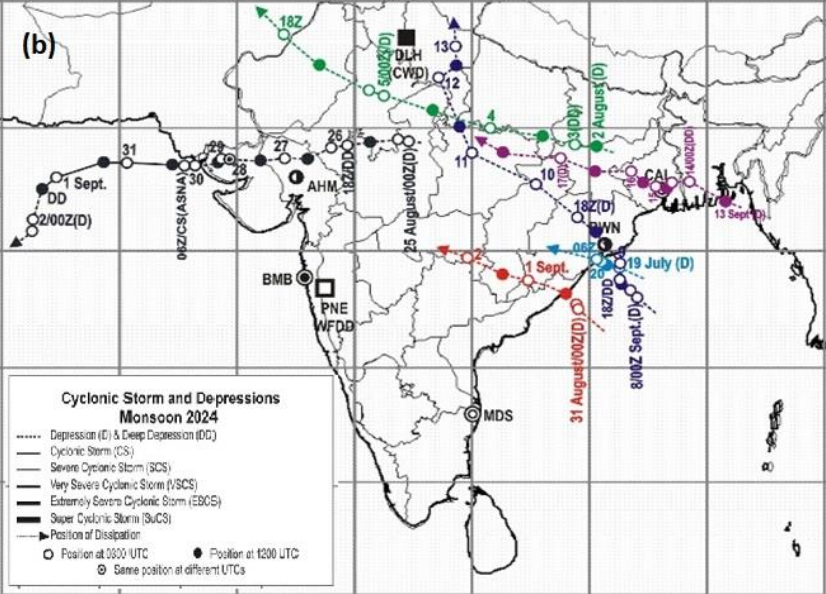
\includegraphics[width=1.08\linewidth]{images/IMD-report-2024.png}
            \end{figure}
            \label{fig:imd_report_2024}

            \vspace{0.2cm}
            {\tiny \textbf{Figure~\ref{fig:imd_report_2024} :} IMD Annual Monsoon report 2024 \footnotemark[4]}
        \end{columns}
    \end{center}
\end{frame}

\begin{frame}[label=comparison]{Comparison with IMD Annual Monsoon Report 2024}
    \vspace{-0.1cm}
    \textbf{Analysis Monthly Distribution (2024)}

    \vspace{0.1cm}
    \begin{columns}[T, totalwidth=\textwidth]
        \column{0.48\textwidth}
        \footnotesize
        \begin{block}{ERA5 Single Level Dataset}
            \begin{tabular}{p{0.4\linewidth} p{0.3\linewidth}}
                \toprule
                Month      & No. of detections  \\
                \midrule
                June      & 0                  \\
                July      & 1 (Track 1)        \\
                August    & 3 (Tracks 2, 3, 4) \\
                September & 2 (Tracks 5, 6)    \\
                \midrule
                Total Detected   & 6           \\
                \bottomrule
            \end{tabular}
        \end{block}

        \column{0.48\textwidth}
        \footnotesize
        \begin{block}{IMD Monsoon Report 2024}
            \begin{tabular}{p{0.4\linewidth} p{0.3\linewidth}}
                \toprule
                Month      & No. of detections          \\
                \midrule
                June      & 0                          \\
                July      & 1                          \\
                August    & 3                          \\
                September & 2                          \\
                \midrule
                Total reported (D + DD)\footnotemark[5] & 6 \\
                \bottomrule
            \end{tabular}
        \end{block}
    \end{columns}

    \vspace{0.6cm}
    \begin{columns}[T, onlytextwidth]
        \column{0.48\textwidth}
        \footnotesize
        \centering
        \begin{block}{Temporal Resolution}
            \begin{tabular}{p{0.4\linewidth} p{0.3\linewidth}}
                \toprule
                Source & Temporal resolution\\
                \midrule
                \textbf{IMD} & \texttt{3-hourly} tracking \\
                \textbf{ERA5} & \texttt{1-hourly} tracking \\
                \bottomrule
            \end{tabular}
        \end{block}

        \column{0.48\textwidth}
        \footnotesize
        \centering
        \begin{block}{MD Spatial Origin}
            \begin{tabular}{p{0.4\linewidth} p{0.3\linewidth}}
                \toprule
                Origin       & Tracks \\
                \midrule
                \textbf{Ocean-Origin} & \texttt{3} (Tracks 1, 4, 5) \\
                \textbf{Land-Origin} & \texttt{3} (Tracks 2, 3, 6) \\
                \bottomrule
            \end{tabular}
        \end{block}
    \end{columns}

    \vspace{0.6cm}
    \begin{center}
        \footnotesize
        \textbf{Validation Result :} All match in monthly frequency and total count with just small temporal difference in start and end time for some tracks.
    \end{center}

    \vfill
    \footnotetext[5]{\tiny D $\rightarrow$ Depression and DD $\rightarrow$ Deep Depression}
\end{frame}

% \begin{frame}{Overall Statistics \& Track Details}
%     \vspace{-0.8cm}
%     \begin{center}
%         \begin{block}{Track Characteristics}
%             \vspace{0.3cm}
%             \centering
%             \footnotesize
%             \begin{tabular}{p{0.033\linewidth} p{0.085\linewidth} p{0.106\linewidth} p{0.135\linewidth} p{0.108\linewidth} p{0.107\linewidth} p{0.100\linewidth}}
%                 % \begin{tabular}{@{}clclllll@{}}
%                 \toprule
%                                   & \multicolumn{4}{c}{\textbf{Detection using ERA5 data}} & \multicolumn{2}{c}{\textbf{IMD Monsoon Report 2024}}                                                                                                                                                                   \\
%                 \cmidrule(lr){2-5} \cmidrule(lr){6-7}
%                 \textbf{Track ID} & \textbf{Origin}                                        & \textbf{Time (2024)}                                 & \textbf{Detected Duration} & \textbf{Category\footnotemark[6] \tiny{($\geq$96h (4 days))}} & \textbf{IMD reported time (2024)} & \textbf{IMD reported duration} \\
%                 \midrule
%                 1                 & Over Ocean                                             & 18/07 04:00 - 21/07 07:00                            & 75h ($\sim$ 3 days)        & Short-lived                                                   & 19/07 - 20/07                     & 3 days                         \\
%                 2                 & Over Land                                              & 01/08 19:00 - 06/08 04:00                            & 106h ($\sim$ 4.5 days)     & Long-lived                                                    & 02/08 - 06/08                     & 4 days                         \\
%                 3                 & Over Land                                              & 23/08 08:00 - 29/08 10:00                            & 146h ($\sim$ 6 days)       & Long-lived                                                    & 25/08 - 01/09                     & 8 days                         \\
%                 4                 & Over Ocean                                             & 30/08 05:00 - 02/09 08:00                            & 75h ($\sim$ 3 days)        & Short-lived                                                   & 31/08 - 02/09                     & 3 days                         \\
%                 5                 & Over Ocean                                             & 06/09 06:00 - 13/09 03:00                            & 165h ($\sim$ 7 days)       & Long-lived                                                    & 08/09 - 13/09                     & 5 days                         \\
%                 6                 & Over Land                                              & 13/09 12:00 - 18/09 07:00                            & 115h ($\sim$ 5 days)       & Long-lived                                                    & 13/09 - 18/09                     & 5 days                         \\
%                 \bottomrule
%             \end{tabular}
%         \end{block}
%         \tiny \textit{Mean Detection Duration for all tracks is $115.2 \pm 38.3$ hours.}
%     \end{center}
%
%     \vspace{-0.6cm}
%     \footnotetext[6]{\tiny Short or long lived MDs are Categorized based on their duration less or more than $96$ hours ($\sim 4$ days)}
% \end{frame}

% %%%%%%%%%%%%%%%%%%%%%%%%
% % TODO: add ASM and FSI comparison for all tracks
% % \begin{frame}{Track Comparison: ASM vs FSI}
% %     \begin{columns}[T, onlytextwidth]
% %         \column{0.48\textwidth}
% %         \begin{center}
% %             \includegraphics[width=0.95\textwidth]{figures/h3_scatter.png}
% %             \\[0.2cm]
% %             {\tiny \textbf{Figure 5:} Scatter plot of antecedent soil moisture (x-axis, m³/m³) versus feedback strength index (y-axis). The strong positive correlation (r = 0.921)  strongly supports H3 hypothesis. Wetter pre-monsoon soils predict stronger land-atmosphere coupling during depression passage.}
% %         \end{center}
% %
% %         \column{0.48\textwidth}
% %         \begin{center}
% %             \includegraphics[width=0.95\textwidth]{figures/track_5_anomaly.png}
% %             \\[0.2cm]
% %             {\tiny \textbf{Figure 6:} Close-up of Track 5 anomaly. Despite moderate-to-wet antecedent soil moisture (ASM = 0.319 m³/m³), this depression exhibited unusually weak coupling (FSI = 0.210). Possible explanations: wind shear suppression, cooler SST, or data quality issues. Requires detailed case study.}
% %         \end{center}
% %     \end{columns}
% % \end{frame}
% %%%%%%%%%%%%%%%%%%%%%%%%

%%%%%%%%%%%%%%% Track 1 %%%%%%%%%%%%%%
\subsection{Track 1}
\subsubsection{Track 1 Details}
\begin{frame}{Track 1 Details}
    \vspace{-0.1cm}
    \begin{center}
        \begin{columns}[T]
            \column{0.5\textwidth}
            \includegraphics[width=0.9\textwidth]{../version21-with-no-ocean-masking/output_2024/track_1/MD_track_1_detailed.png}

            \vspace{0.05cm}
            \footnotesize
            \begin{block}{Statistics}
                \begin{itemize}
                    \item Duration : 78 hours ($\sim$ 3 days)
                    \item Category : short-lived MD
                    \item Origin : Bay of Bengal (Oceanic)
                \end{itemize}
            \end{block}

            \column{0.5\textwidth}
            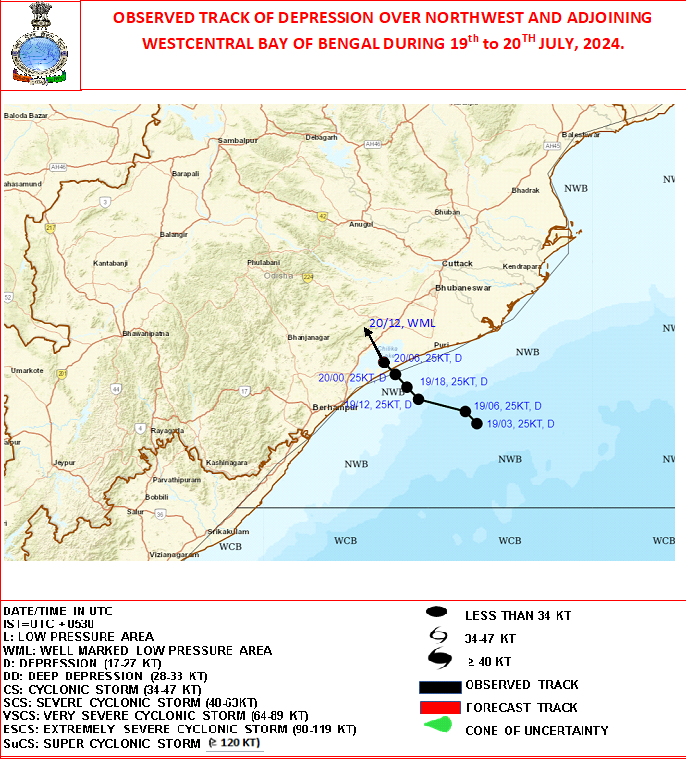
\includegraphics[width=0.8\textwidth]{images/July-19-20-2024.png}

            \footnote{\tiny Source RSMC New Delhi Report 2024 : \href{https://rsmcnewdelhi.imd.gov.in/report.php?internal\_menu=MzQ=}{\url{https://rsmcnewdelhi.imd.gov.in/report.php?internal\_menu=MzQ=}}}
        \end{columns}
    \end{center}
\end{frame}

\subsubsection{Track 1 Translation Speed}
\begin{frame}{Track 1 Translation speed of MD}
    \begin{center}
        \includegraphics[width=0.8\textwidth]{../version21-with-no-ocean-masking/output_2024/track_1/translational-speed/track_1_speed_ms.png}
    \end{center}
\end{frame}

\subsubsection{Track 1 HF Time evolution}
\begin{frame}{Track 1 Heat Flux evolution}
    \begin{center}
        \begin{figure}
            \includegraphics[width=0.6\textwidth]{../version21-with-no-ocean-masking/output_2024/track_1/time_series/track_1_heat_flux_time_series.png}
        \end{figure}
        \label{fig:track_1_heat_flux_timeseries}
    \end{center}

    \vspace{0.2cm}
    {\tiny \textbf{Figure~\ref{fig:track_1_heat_flux_timeseries} :} Time series of sensible, latent, and total heat fluxes for Track 1}% Note the dramatic increase in total heat flux upon landfall, primarily driven by latent heat component. This energy influx sustains the depression over land.}
\end{frame}

\subsubsection{Track 1 TP and SWVL1 Time evolution}
\begin{frame}{Track 1 \texttt{TP} and \texttt{SWVL1} Time evolution}
       \begin{figure}
           \centering
           \includegraphics[width=\textwidth]{../version21-with-no-ocean-masking/output_2024/track_1/time_series/track_1_TP-SWVL1_time_series.png}
       \end{figure}
       \label{fig:track_1_TP-SWVL1_time_series}

       % TODO:
       \vspace{0.2cm}
       {\tiny Figure~\ref{fig:track_1_TP-SWVL1_time_series} : Temporal evolution of \texttt{TP} and \texttt{SWVL1}. The vertical dashed line indicates landfall time} %([date/time])}. Key observation: [Variable] increases by X units upon landfall, supporting the hypothesis that [physical mechanism]. This pattern was consistent across all 6 depressions analyzed.}
\end{frame}

\subsubsection{Track 1 - Auto-Correlations}
\begin{frame}{Track 1 - \texttt{SWVL1} and \texttt{TP} Auto-Correlation}
    \begin{columns}[T]
        \begin{column}{0.5\textwidth}
            \begin{figure}
                \centering
                \includegraphics[width=\textwidth]{../version21-with-no-ocean-masking/output_2024/track_1/correlation_analysis/autocorrelation/track_1_autocorr_swvl1.png}
            \end{figure}
            \label{fig:track_1_SWVL1_autocorrelation}

            % TODO:
            \vspace{0.2cm}
            {\tiny \textbf{Figure~\ref{fig:track_1_SWVL1_autocorrelation} :}Auto-correlation of soil moisture (\texttt{SWVL1})  for Track 1.} % Maximum correlation of r = [X] occurs at lag [Y hours], suggesting that soil moisture response lags precipitation by approximately [Y hours]. This lag is consistent with water infiltration timescales in the region.}
        \end{column}

        \begin{column}{0.5\textwidth}
            \begin{figure}
                \centering
                \includegraphics[width=\textwidth]{../version21-with-no-ocean-masking/output_2024/track_1/correlation_analysis/autocorrelation/track_1_autocorr_tp.png}
            \end{figure}
            \label{fig:track_1_TP_autocorrelation}

            % TODO:
            \vspace{0.2cm}
            {\tiny \textbf{Figure~\ref{fig:track_1_TP_autocorrelation} :}Auto-correlation of Total precipitation (\texttt{TP}) for Track 1.} % Maximum correlation of r = [X] occurs at lag [Y hours], suggesting that soil moisture response lags precipitation by approximately [Y hours]. This lag is consistent with water infiltration timescales in the region.}
        \end{column}

        % \begin{column}{0.4\textwidth}
        %     \footnotesize
        %     \textbf{Summary:}
        %     \begin{itemize}
        %         \item The peak of correlation occurs at far left of zero-lag line (24 hours earlier).
        %         \item Antecedent moisture, Soil moisture levels are precursor to rainfall (or say sets condition for rainfall) events 24 hours later.
        %         \item Suggests very slow moving land-atmosphere feedback loop.
        %     \end{itemize}
        % \end{column}
    \end{columns}
\end{frame}

\begin{frame}{Track 1 - HF Auto-Correlation}
    \vspace{-0.3cm}
    \begin{columns}[T]
        \begin{column}{0.45\textwidth}
            \begin{figure}
                \centering
                \includegraphics[width=\textwidth]{../version21-with-no-ocean-masking/output_2024/track_1/correlation_analysis/autocorrelation/track_1_autocorr_latent_hf.png}
            \end{figure}
            \label{fig:track_1_LHF_autocorrelation}
        \end{column}

        \begin{column}{0.45\textwidth}
            \begin{figure}
                \centering
                \includegraphics[width=\textwidth]{../version21-with-no-ocean-masking/output_2024/track_1/correlation_analysis/autocorrelation/track_1_autocorr_sensible_hf.png}
            \end{figure}
            \label{fig:track_1_SHF_autocorrelation}
        \end{column}

        % \begin{column}{0.45\textwidth}
        %     \footnotesize
        %     \textbf{Summary:}
        %     \begin{itemize}
        %     \end{itemize}
        % \end{column}
    \end{columns}

    \vspace{-0.3cm}
    \begin{columns}[T]
        \begin{column}{0.45\textwidth}
            \begin{figure}
                \centering
                \includegraphics[width=\textwidth]{../version21-with-no-ocean-masking/output_2024/track_1/correlation_analysis/autocorrelation/track_1_autocorr_total_hf.png}
            \end{figure}
            \label{fig:track_1_THF_autocorrelation}
        \end{column}

        \begin{column}{0.45\textwidth}
            % TODO:
            \vspace{1.5cm}
            {\tiny \textbf{Figures :} Auto-correlation of Heat fluxes (\texttt{LHF, SHF} and \texttt{THF}) for Track 1.} % Maximum correlation of r = [X] occurs at lag [Y hours], suggesting that soil moisture response lags precipitation by approximately [Y hours]. This lag is consistent with water infiltration timescales in the region.}
        \end{column}
    \end{columns}
\end{frame}

\begin{frame}{Track 1 - \texttt{SWVL1-HF} Correlation}
    \vspace{-0.5cm}
    \begin{columns}[T]
        \begin{column}{0.8\textwidth}
            \begin{figure}
                \centering
                \includegraphics[width=\textwidth]{../version21-with-no-ocean-masking/output_2024/track_1/correlation_analysis/correlation/track_1_SWVL1-HF_correlation.png}
            \end{figure}
            \label{fig:track_1_swvl1-hf_correlation}

            \vspace{-0.4cm}
            \begin{figure}
                \centering
                \includegraphics[width=\textwidth]{../version21-with-no-ocean-masking/output_2024/track_1/correlation_analysis/correlation/track_1_TP-HF_correlation.png}
            \end{figure}
            \label{fig:track_1_tp-hf_correlation}
        \end{column}

        \begin{column}{0.2\textwidth}
        %     \footnotesize
        %     \textbf{Summary:}
        %     \begin{itemize}
        %         \item The peak of correlation occurs at far left of zero-lag line (24 hours earlier).
        %         \item Antecedent moisture, Soil moisture levels are precursor to rainfall (or say sets condition for rainfall) events 24 hours later.
        %         \item Suggests very slow moving land-atmosphere feedback loop.
        %     \end{itemize}
        \end{column}
    \end{columns}

    % \vspace{-0.3cm}
    % \begin{columns}[T]
    %     \begin{column}{0.45\textwidth}
    %
    %     \end{column}
    %
    %     \begin{column}{0.45\textwidth}
    %         % TODO:
    %         \vspace{1.5cm}
    %         {\tiny \textbf{Figures :} Correlation for Track 1.} % Maximum correlation of r = [X] occurs at lag [Y hours], suggesting that soil moisture response lags precipitation by approximately [Y hours]. This lag is consistent with water infiltration timescales in the region.}
    %     \end{column}
    % \end{columns}
\end{frame}

\subsubsection{Track 1 TP-SWVL1 Correlation}
\begin{frame}{Track 1 \texttt{TP-SWVL1} Correlation}
    \begin{columns}[T]
        \begin{column}{0.6\textwidth}
            \begin{figure}
                \centering
                \includegraphics[width=\textwidth]{../version21-with-no-ocean-masking/output_2024/track_1/correlation_analysis/correlation/track_1_TP-SWVL1_correlation.png}
            \end{figure}
            \label{fig:track_1_tp-swvl1_correlation}
        \end{column}

        \begin{column}{0.4\textwidth}
            \footnotesize
        %     \textbf{Statistical Summary :}
        %     \begin{itemize}
        %         \item \textbf{Pearson r :} \texttt{-0.2633} – Weak negative linear relationship between precipitation and soil moisture more rainfall leads lower soil moisture (why? 1. maybe because track is short-lived, 2. MD doesn't penetrate inland deep). \cite{kishtawal2013enhancement}
        %         \item \textbf{Spearman $\rho$ :} \texttt{-0.2930} – slight negative monotonic trend suggests higher rain corresponds to lower simultaneous soil moisture.
        %         \item \textbf{p-value :} \texttt{3.0054 \times 10$^{-2}$} – Statistically significant ($p < 0.05$), though the correlation strength is low.
        %         \item \textbf{Mean TP :} 0.49 $mm/hr$
        %         \item \textbf{Mean SM :} 0.14 m$^3$/m$^3$
        %     \end{itemize}
        \end{column}
    \end{columns}
\end{frame}

\begin{frame}{Track 1 - \texttt{TP-SWVL1} Lag Correlation}
    \begin{columns}[T]
        \begin{column}{0.6\textwidth}
            \begin{figure}
                \centering
                \includegraphics[width=\textwidth]{../version21-with-no-ocean-masking/output_2024/track_1/correlation_analysis/lag_correlation/track_1_TP-SWVL1_lag_correlation.png}
            \end{figure}
            \label{fig:track_1_TP-SWVL1_lag_correlation}

            % TODO:
            \vspace{0.2cm}
            {\tiny \textbf{Figure~\ref{fig:track_1_TP-SWVL1_lag_correlation} :}Lag correlation between precipitation (\texttt{TP}) and soil moisture (\texttt{SWVL1})  for Track 1.} % Maximum correlation of r = [X] occurs at lag [Y hours], suggesting that soil moisture response lags precipitation by approximately [Y hours]. This lag is consistent with water infiltration timescales in the region.}
        \end{column}

        % \begin{column}{0.4\textwidth}
        %     \footnotesize
        %     \textbf{Summary:}
        %     \begin{itemize}
        %         \item The peak of correlation occurs at far left of zero-lag line (24 hours earlier).
        %         \item Antecedent moisture, Soil moisture levels are precursor to rainfall (or say sets condition for rainfall) events 24 hours later.
        %         \item Suggests very slow moving land-atmosphere feedback loop.
        %     \end{itemize}
        % \end{column}
    \end{columns}
\end{frame}

\begin{frame}{Track 1 \texttt{SWVL1-HF} Lag Correlation}
    \begin{columns}[t]
        \begin{column}{0.5\textwidth}
            \begin{center}
                \includegraphics[width=0.9\textwidth]{../version21-with-no-ocean-masking/output_2024/track_1/correlation_analysis/lag_correlation/track_1_SWVL1-LHF_lag_correlation.png} \\
                \includegraphics[width=0.9\textwidth]{../version21-with-no-ocean-masking/output_2024/track_1/correlation_analysis/lag_correlation/track_1_SWVL1-SHF_lag_correlation.png}
            \end{center}
        \end{column}

        \begin{column}{0.5\textwidth}
            \begin{center}
                \includegraphics[width=0.9\textwidth]{../version21-with-no-ocean-masking/output_2024/track_1/correlation_analysis/lag_correlation/track_1_SWVL1-THF_lag_correlation.png}
            \end{center}
        \end{column}
    \end{columns}
\end{frame}

\begin{frame}{Track 1 \texttt{TP-HF} Lag Correlation}
    \begin{columns}[t]
        \begin{column}{0.5\textwidth}
            \begin{center}
                \includegraphics[width=0.9\textwidth]{../version21-with-no-ocean-masking/output_2024/track_1/correlation_analysis/lag_correlation/track_1_TP-LHF_lag_correlation.png} \\
                \includegraphics[width=0.9\textwidth]{../version21-with-no-ocean-masking/output_2024/track_1/correlation_analysis/lag_correlation/track_1_TP-SHF_lag_correlation.png}
            \end{center}
        \end{column}

        \begin{column}{0.5\textwidth}
            \begin{center}
                \includegraphics[width=0.9\textwidth]{../version21-with-no-ocean-masking/output_2024/track_1/correlation_analysis/lag_correlation/track_1_TP-THF_lag_correlation.png}
            \end{center}
        \end{column}
    \end{columns}
\end{frame}

\subsubsection{Track 1 Hovm\"oller plots}
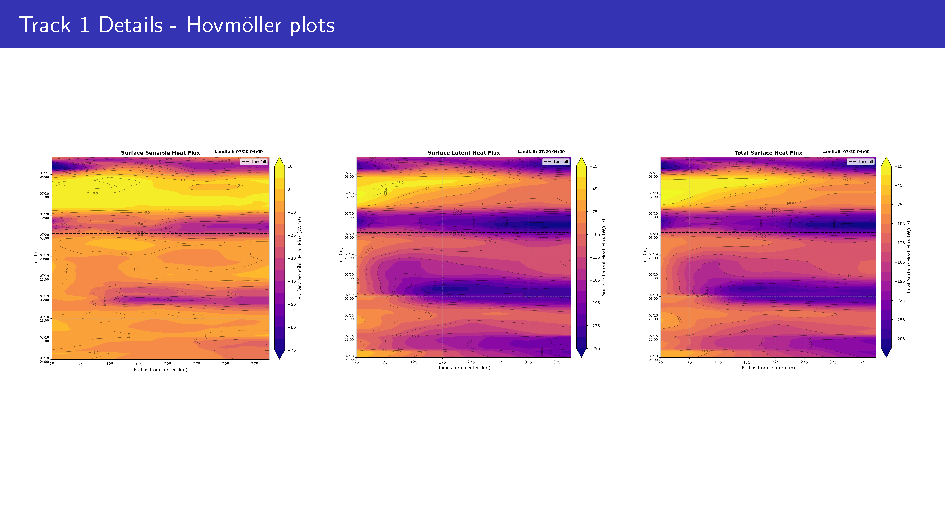
\includepdf[
    pages=-,
    scale=1,
    frame=true,
    % pagecommand={},
    pagecommand={\stepcounter{framenumber}},
    offset=0mm 0mm,       % Adjust position
    % templatesize={\textwidth}{\textheight} % Match template size
]{slides/hov-1.pdf}

\subsubsection{Track 1 \texttt{MODIS}}
\begin{frame}{\texttt{MODIS} Track 1 Visualization (2000m Scale)}
    \begin{center}
        \begin{figure}
            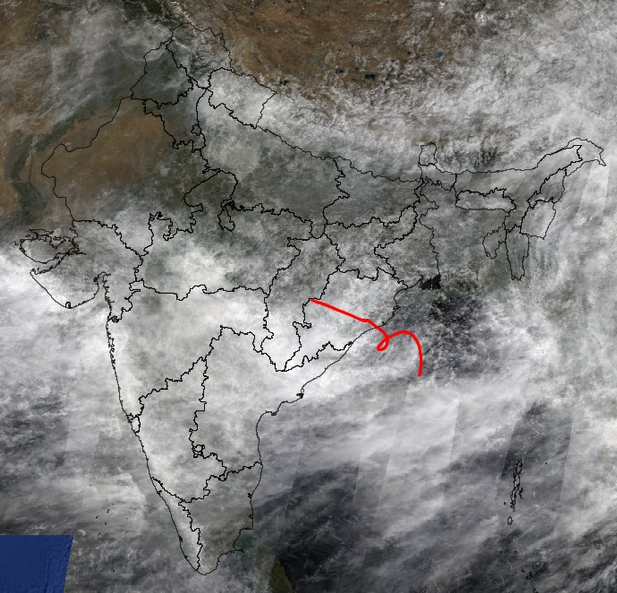
\includegraphics[width=0.45\linewidth]{images/MODIS-2024-Track_1.png}
        \end{figure}
        \label{fig:modistrack1}
    \end{center}

    \vspace{0.2cm}
    {\tiny \textbf{Figure~\ref{fig:modistrack1} :} \texttt{MODIS} satellite image (true color) of Track. The characteristic depression cloud structure is visible with high Cloud cluster to the southwest of track. Image source: GEE, NASA \texttt{MODIS} Level 1B.}
\end{frame}

% %%%%%%%%%%%%%%%% Track 2 %%%%%%%%%%%%%%
\subsection{Track 2}
\subsubsection{Track 2 Details}
\begin{frame}{Track 2 Details}
    \vspace{-0.1cm}
    \begin{center}
        \begin{columns}[T]
            \column{0.5\textwidth}
            \includegraphics[width=0.9\textwidth]{../version21-with-no-ocean-masking/output_2024/track_2/MD_track_2_detailed.png}

            \vspace{0.05cm}
            \footnotesize
            \begin{block}{Statistics}
                \begin{itemize}
                    \item Duration: 106 hours ($\sim$ 4.5 days)
                    \item Category: long-lived MD
                    \item Originated: over land
                \end{itemize}
            \end{block}

            \column{0.5\textwidth}
            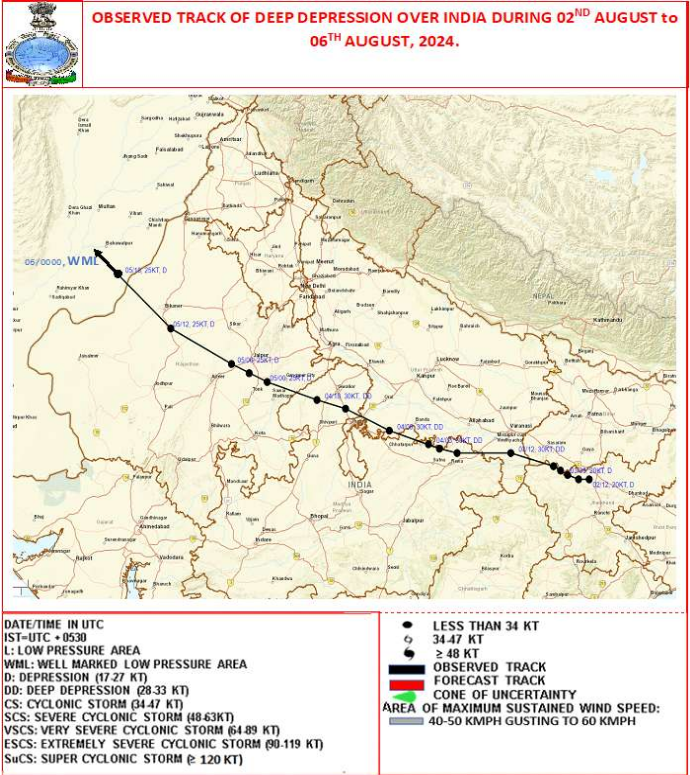
\includegraphics[width=0.8\textwidth]{images/August-02-06-2024.png}

            \footnote{\tiny Source RSMC New Delhi Report 2024 : \href{https://rsmcnewdelhi.imd.gov.in/report.php?internal_menu=MzQ=}{\url{https://rsmcnewdelhi.imd.gov.in/report.php?internal_menu=MzQ=}}}
        \end{columns}
    \end{center}
    % Source : https://rsmcnewdelhi.imd.gov.in/download.php?path=uploads/archive/1/1_bf848c_18.%20National%20Bulletin%20No%2018-06Aug2024_0530IST.pdf
\end{frame}

\subsubsection{Track 2 Translation Speed}
\begin{frame}{Track 2 Translation speed of MD}
    \begin{center}
        \includegraphics[width=0.8\textwidth]{../version21-with-no-ocean-masking/output_2024/track_2/translational-speed/track_2_speed_ms.png}
    \end{center}
\end{frame}

\subsubsection{Track 2 HF Time evolution}
\begin{frame}{Track 2 Heat Flux evolution}
    \begin{center}
        \begin{figure}
            \includegraphics[width=0.6\textwidth]{../version21-with-no-ocean-masking/output_2024/track_2/time_series/track_2_heat_flux_time_series.png}
        \end{figure}
        \label{fig:track_2_heat_flux_timeseries}
    \end{center}

    \vspace{0.2cm}
    {\tiny \textbf{Figure~\ref{fig:track_2_heat_flux_timeseries} :} Time series of sensible, latent, and total heat fluxes for Track 2}% Note the dramatic increase in total heat flux upon landfall, primarily driven by latent heat component. This energy influx sustains the depression over land.}
\end{frame}

\subsubsection{Track 2 TP and SWVL1 Time evolution}
\begin{frame}{Track 2 \texttt{TP} and \texttt{SWVL1} Time evolution}
       \begin{figure}
           \centering
           \includegraphics[width=\textwidth]{../version21-with-no-ocean-masking/output_2024/track_2/time_series/track_2_TP-SWVL1_time_series.png}
       \end{figure}
       \label{fig:track_2_TP-SWVL1_time_series}

       % TODO:
       \vspace{0.2cm}
       {\tiny Figure~\ref{fig:track_2_TP-SWVL1_time_series} : Temporal evolution of \texttt{TP} and \texttt{SWVL1}. The vertical dashed line indicates landfall time} %([date/time])}. Key observation: [Variable] increases by X units upon landfall, supporting the hypothesis that [physical mechanism]. This pattern was consistent across all 6 depressions analyzed.}
\end{frame}

\subsubsection{Track 2 - Auto-Correlations}
\begin{frame}{Track 2 - \texttt{SWVL1} and \texttt{TP} Auto-Correlation}
    \begin{columns}[T]
        \begin{column}{0.5\textwidth}
            \begin{figure}
                \centering
                \includegraphics[width=\textwidth]{../version21-with-no-ocean-masking/output_2024/track_2/correlation_analysis/autocorrelation/track_2_autocorr_swvl1.png}
            \end{figure}
            \label{fig:track_2_SWVL1_autocorrelation}

            % TODO:
            \vspace{0.2cm}
            {\tiny \textbf{Figure~\ref{fig:track_2_SWVL1_autocorrelation} :}Auto-correlation of soil moisture (\texttt{SWVL1})  for Track 2.} % Maximum correlation of r = [X] occurs at lag [Y hours], suggesting that soil moisture response lags precipitation by approximately [Y hours]. This lag is consistent with water infiltration timescales in the region.}
        \end{column}

        \begin{column}{0.5\textwidth}
            \begin{figure}
                \centering
                \includegraphics[width=\textwidth]{../version21-with-no-ocean-masking/output_2024/track_2/correlation_analysis/autocorrelation/track_2_autocorr_tp.png}
            \end{figure}
            \label{fig:track_2_TP_autocorrelation}

            % TODO:
            \vspace{0.2cm}
            {\tiny \textbf{Figure~\ref{fig:track_2_TP_autocorrelation} :}Auto-correlation of Total precipitation (\texttt{TP}) for Track 2.} % Maximum correlation of r = [X] occurs at lag [Y hours], suggesting that soil moisture response lags precipitation by approximately [Y hours]. This lag is consistent with water infiltration timescales in the region.}
        \end{column}

        % \begin{column}{0.4\textwidth}
        %     \footnotesize
        %     \textbf{Summary:}
        %     \begin{itemize}
        %         \item The peak of correlation occurs at far left of zero-lag line (24 hours earlier).
        %         \item Antecedent moisture, Soil moisture levels are precursor to rainfall (or say sets condition for rainfall) events 24 hours later.
        %         \item Suggests very slow moving land-atmosphere feedback loop.
        %     \end{itemize}
        % \end{column}
    \end{columns}
\end{frame}

\begin{frame}{Track 2 - HF Auto-Correlation}
    \vspace{-0.3cm}
    \begin{columns}[T]
        \begin{column}{0.45\textwidth}
            \begin{figure}
                \centering
                \includegraphics[width=\textwidth]{../version21-with-no-ocean-masking/output_2024/track_2/correlation_analysis/autocorrelation/track_2_autocorr_latent_hf.png}
            \end{figure}
            \label{fig:track_2_LHF_autocorrelation}
        \end{column}

        \begin{column}{0.45\textwidth}
            \begin{figure}
                \centering
                \includegraphics[width=\textwidth]{../version21-with-no-ocean-masking/output_2024/track_2/correlation_analysis/autocorrelation/track_2_autocorr_sensible_hf.png}
            \end{figure}
            \label{fig:track_2_SHF_autocorrelation}
        \end{column}

        % \begin{column}{0.45\textwidth}
        %     \footnotesize
        %     \textbf{Summary:}
        %     \begin{itemize}
        %     \end{itemize}
        % \end{column}
    \end{columns}

    \vspace{-0.3cm}
    \begin{columns}[T]
        \begin{column}{0.45\textwidth}
            \begin{figure}
                \centering
                \includegraphics[width=\textwidth]{../version21-with-no-ocean-masking/output_2024/track_2/correlation_analysis/autocorrelation/track_2_autocorr_total_hf.png}
            \end{figure}
            \label{fig:track_2_THF_autocorrelation}
        \end{column}

        \begin{column}{0.45\textwidth}
            % TODO:
            \vspace{1.5cm}
            {\tiny \textbf{Figures :} Auto-correlation of Heat fluxes (\texttt{LHF, SHF} and \texttt{THF}) for Track 2.} % Maximum correlation of r = [X] occurs at lag [Y hours], suggesting that soil moisture response lags precipitation by approximately [Y hours]. This lag is consistent with water infiltration timescales in the region.}
        \end{column}
    \end{columns}
\end{frame}

\begin{frame}{Track 2 - \texttt{SWVL1-HF} Correlation}
    \vspace{-0.5cm}
    \begin{columns}[T]
        \begin{column}{0.8\textwidth}
            \begin{figure}
                \centering
                \includegraphics[width=\textwidth]{../version21-with-no-ocean-masking/output_2024/track_2/correlation_analysis/correlation/track_2_SWVL1-HF_correlation.png}
            \end{figure}
            \label{fig:track_2_swvl1-hf_correlation}

            \vspace{-0.4cm}
            \begin{figure}
                \centering
                \includegraphics[width=\textwidth]{../version21-with-no-ocean-masking/output_2024/track_2/correlation_analysis/correlation/track_2_TP-HF_correlation.png}
            \end{figure}
            \label{fig:track_2_tp-hf_correlation}
        \end{column}

        \begin{column}{0.2\textwidth}
        %     \footnotesize
        %     \textbf{Summary:}
        %     \begin{itemize}
        %         \item The peak of correlation occurs at far left of zero-lag line (24 hours earlier).
        %         \item Antecedent moisture, Soil moisture levels are precursor to rainfall (or say sets condition for rainfall) events 24 hours later.
        %         \item Suggests very slow moving land-atmosphere feedback loop.
        %     \end{itemize}
        \end{column}
    \end{columns}

    % \vspace{-0.3cm}
    % \begin{columns}[T]
    %     \begin{column}{0.45\textwidth}
    %
    %     \end{column}
    %
    %     \begin{column}{0.45\textwidth}
    %         % TODO:
    %         \vspace{1.5cm}
    %         {\tiny \textbf{Figures :} Correlation for Track 2.} % Maximum correlation of r = [X] occurs at lag [Y hours], suggesting that soil moisture response lags precipitation by approximately [Y hours]. This lag is consistent with water infiltration timescales in the region.}
    %     \end{column}
    % \end{columns}
\end{frame}

\subsubsection{Track 2 TP-SWVL1 Correlation}
\begin{frame}{Track 2 \texttt{TP-SWVL1} Correlation}
    \begin{columns}[T]
        \begin{column}{0.6\textwidth}
            \begin{figure}
                \centering
                \includegraphics[width=\textwidth]{../version21-with-no-ocean-masking/output_2024/track_2/correlation_analysis/correlation/track_2_TP-SWVL1_correlation.png}
            \end{figure}
            \label{fig:track_2_tp-swvl1_correlation}
        \end{column}

        \begin{column}{0.4\textwidth}
            \footnotesize
        %     \textbf{Statistical Summary :}
        %     \begin{itemize}
        %         \item \textbf{Pearson r :} \texttt{-0.2633} – Weak negative linear relationship between precipitation and soil moisture more rainfall leads lower soil moisture (why? 1. maybe because track is short-lived, 2. MD doesn't penetrate inland deep). \cite{kishtawal2013enhancement} 
        %         \item \textbf{Spearman $\rho$ :} \texttt{-0.2930} – slight negative monotonic trend suggests higher rain corresponds to lower simultaneous soil moisture.
        %         \item \textbf{p-value :} \texttt{3.0054 \times 10$^{-2}$} – Statistically significant ($p < 0.05$), though the correlation strength is low.
        %         \item \textbf{Mean TP :} 0.49 $mm/hr$
        %         \item \textbf{Mean SM :} 0.14 m$^3$/m$^3$
        %     \end{itemize}
        \end{column}
    \end{columns}
\end{frame}

\begin{frame}{Track 2 - \texttt{TP-SWVL1} Lag Correlation}
    \begin{columns}[T]
        \begin{column}{0.6\textwidth}
            \begin{figure}
                \centering
                \includegraphics[width=\textwidth]{../version21-with-no-ocean-masking/output_2024/track_2/correlation_analysis/lag_correlation/track_2_TP-SWVL1_lag_correlation.png}
            \end{figure}
            \label{fig:track_2_TP-SWVL1_lag_correlation}

            % TODO:
            \vspace{0.2cm}
            {\tiny \textbf{Figure~\ref{fig:track_2_TP-SWVL1_lag_correlation} :}Lag correlation between precipitation (\texttt{TP}) and soil moisture (\texttt{SWVL1})  for Track 2.} % Maximum correlation of r = [X] occurs at lag [Y hours], suggesting that soil moisture response lags precipitation by approximately [Y hours]. This lag is consistent with water infiltration timescales in the region.}
        \end{column}

        % \begin{column}{0.4\textwidth}
        %     \footnotesize
        %     \textbf{Summary:}
        %     \begin{itemize}
        %         \item The peak of correlation occurs at far left of zero-lag line (24 hours earlier).
        %         \item Antecedent moisture, Soil moisture levels are precursor to rainfall (or say sets condition for rainfall) events 24 hours later.
        %         \item Suggests very slow moving land-atmosphere feedback loop.
        %     \end{itemize}
        % \end{column}
    \end{columns}
\end{frame}

\begin{frame}{Track 2 \texttt{SWVL1-HF} Lag Correlation}
    \begin{columns}[t]
        \begin{column}{0.5\textwidth}
            \begin{center}
                \includegraphics[width=0.9\textwidth]{../version21-with-no-ocean-masking/output_2024/track_2/correlation_analysis/lag_correlation/track_2_SWVL1-LHF_lag_correlation.png} \\
                \includegraphics[width=0.9\textwidth]{../version21-with-no-ocean-masking/output_2024/track_2/correlation_analysis/lag_correlation/track_2_SWVL1-SHF_lag_correlation.png}
            \end{center}
        \end{column}

        \begin{column}{0.5\textwidth}
            \begin{center}
                \includegraphics[width=0.9\textwidth]{../version21-with-no-ocean-masking/output_2024/track_2/correlation_analysis/lag_correlation/track_2_SWVL1-THF_lag_correlation.png}
            \end{center}
        \end{column}
    \end{columns}
\end{frame}

\begin{frame}{Track 2 \texttt{TP-HF} Lag Correlation}
    \begin{columns}[t]
        \begin{column}{0.5\textwidth}
            \begin{center}
                \includegraphics[width=0.9\textwidth]{../version21-with-no-ocean-masking/output_2024/track_2/correlation_analysis/lag_correlation/track_2_TP-LHF_lag_correlation.png} \\
                \includegraphics[width=0.9\textwidth]{../version21-with-no-ocean-masking/output_2024/track_2/correlation_analysis/lag_correlation/track_2_TP-SHF_lag_correlation.png}
            \end{center}
        \end{column}

        \begin{column}{0.5\textwidth}
            \begin{center}
                \includegraphics[width=0.9\textwidth]{../version21-with-no-ocean-masking/output_2024/track_2/correlation_analysis/lag_correlation/track_2_TP-THF_lag_correlation.png}
            \end{center}
        \end{column}
    \end{columns}
\end{frame}

\subsubsection{Track 2 Hovm\"oller plots}
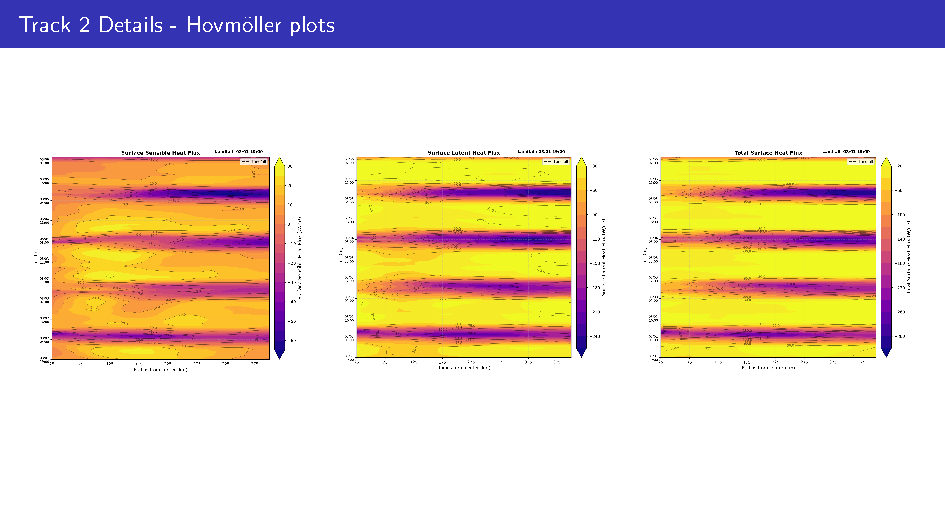
\includepdf[
    pages=-,
    scale=1,
    frame=true,
    % pagecommand={},
    pagecommand={\stepcounter{framenumber}},
    offset=0mm 0mm,       % Adjust position
    % templatesize={\textwidth}{\textheight} % Match template size
]{slides/hov-2.pdf}

\subsubsection{Track 2 \texttt{MODIS}}
\begin{frame}{\texttt{MODIS} Track 2 Visualization (2000m Scale)}
    \begin{center}
        \begin{figure}
            \includegraphics[width=0.45\linewidth]{images/MODIS-2024-Track_2.png}
        \end{figure}
        \label{fig:modistrack2}
    \end{center}

    % TODO:
    \vspace{0.2cm}
    {\tiny \textbf{Figure~\ref{fig:modistrack2} :} \texttt{MODIS} satellite image (true color) of Track. The characteristic depression cloud structure is visible with high Cloud cluster to the around/near track (unlike track 1) because of very low translation speed of MD centre. Image source: GEE, NASA \texttt{MODIS} Level 1B.}
\end{frame}

%%%%%%%%%%%%%%%% Track 3 %%%%%%%%%%%%%%
\subsection{Track 3}
\subsubsection{Track 3 Details}
\begin{frame}{Track 3 Details}
    \vspace{-0.1cm}
    \begin{center}
        \begin{columns}[T]
            \column{0.5\textwidth}
            \includegraphics[width=0.9\textwidth]{../version21-with-no-ocean-masking/output_2024/track_3/MD_track_3_detailed.png}

            \vspace{0.05cm}
            \footnotesize
            \begin{block}{Statistics}
                \begin{itemize}
                    \item Duration: 146 hours ($\sim$ 6 days)
                    \item Category: long-lived MD
                    \item Originated: over land
                \end{itemize}
            \end{block}

            \column{0.5\textwidth}
            % \includegraphics[width=0.95\textwidth]{images/}
        \end{columns}
    \end{center}
\end{frame}

\subsubsection{Track 3 Translation Speed}
\begin{frame}{Track 3 Translation speed of MD}
    \begin{center}
        \includegraphics[width=0.8\textwidth]{../version21-with-no-ocean-masking/output_2024/track_3/translational-speed/track_3_speed_ms.png}
    \end{center}
\end{frame}

\subsubsection{Track 3 HF Time evolution}
\begin{frame}{Track 3 Heat Flux evolution}
    \begin{center}
        \begin{figure}
            \includegraphics[width=0.6\textwidth]{../version21-with-no-ocean-masking/output_2024/track_3/time_series/track_3_heat_flux_time_series.png}
        \end{figure}
        \label{fig:track_3_heat_flux_timeseries}
    \end{center}

    \vspace{0.2cm}
    {\tiny \textbf{Figure~\ref{fig:track_3_heat_flux_timeseries} :} Time series of sensible, latent, and total heat fluxes for Track 3}% Note the dramatic increase in total heat flux upon landfall, primarily driven by latent heat component. This energy influx sustains the depression over land.}
\end{frame}

\subsubsection{Track 3 TP and SWVL1 Time evolution}
\begin{frame}{Track 3 \texttt{TP} and \texttt{SWVL1} Time evolution}
       \begin{figure}
           \centering
           \includegraphics[width=\textwidth]{../version21-with-no-ocean-masking/output_2024/track_3/time_series/track_3_TP-SWVL1_time_series.png}
       \end{figure}
       \label{fig:track_3_TP-SWVL1_time_series}

       % TODO:
       \vspace{0.2cm}
       {\tiny Figure~\ref{fig:track_3_TP-SWVL1_time_series} : Temporal evolution of \texttt{TP} and \texttt{SWVL1}. The vertical dashed line indicates landfall time} %([date/time])}. Key observation: [Variable] increases by X units upon landfall, supporting the hypothesis that [physical mechanism]. This pattern was consistent across all 6 depressions analyzed.}
\end{frame}

\subsubsection{Track 3 - Auto-Correlations}
\begin{frame}{Track 3 - \texttt{SWVL1} and \texttt{TP} Auto-Correlation}
    \begin{columns}[T]
        \begin{column}{0.5\textwidth}
            \begin{figure}
                \centering
                \includegraphics[width=\textwidth]{../version21-with-no-ocean-masking/output_2024/track_3/correlation_analysis/autocorrelation/track_3_autocorr_swvl1.png}
            \end{figure}
            \label{fig:track_3_SWVL1_autocorrelation}

            % TODO:
            \vspace{0.2cm}
            {\tiny \textbf{Figure~\ref{fig:track_3_SWVL1_autocorrelation} :}Auto-correlation of soil moisture (\texttt{SWVL1})  for Track 3.} % Maximum correlation of r = [X] occurs at lag [Y hours], suggesting that soil moisture response lags precipitation by approximately [Y hours]. This lag is consistent with water infiltration timescales in the region.}
        \end{column}

        \begin{column}{0.5\textwidth}
            \begin{figure}
                \centering
                \includegraphics[width=\textwidth]{../version21-with-no-ocean-masking/output_2024/track_3/correlation_analysis/autocorrelation/track_3_autocorr_tp.png}
            \end{figure}
            \label{fig:track_3_TP_autocorrelation}

            % TODO:
            \vspace{0.2cm}
            {\tiny \textbf{Figure~\ref{fig:track_3_TP_autocorrelation} :}Auto-correlation of Total precipitation (\texttt{TP}) for Track 3.} % Maximum correlation of r = [X] occurs at lag [Y hours], suggesting that soil moisture response lags precipitation by approximately [Y hours]. This lag is consistent with water infiltration timescales in the region.}
        \end{column}

        % \begin{column}{0.4\textwidth}
        %     \footnotesize
        %     \textbf{Summary:}
        %     \begin{itemize}
        %         \item The peak of correlation occurs at far left of zero-lag line (24 hours earlier).
        %         \item Antecedent moisture, Soil moisture levels are precursor to rainfall (or say sets condition for rainfall) events 24 hours later.
        %         \item Suggests very slow moving land-atmosphere feedback loop.
        %     \end{itemize}
        % \end{column}
    \end{columns}
\end{frame}

\begin{frame}{Track 3 - HF Auto-Correlation}
    \vspace{-0.3cm}
    \begin{columns}[T]
        \begin{column}{0.45\textwidth}
            \begin{figure}
                \centering
                \includegraphics[width=\textwidth]{../version21-with-no-ocean-masking/output_2024/track_3/correlation_analysis/autocorrelation/track_3_autocorr_latent_hf.png}
            \end{figure}
            \label{fig:track_3_LHF_autocorrelation}
        \end{column}

        \begin{column}{0.45\textwidth}
            \begin{figure}
                \centering
                \includegraphics[width=\textwidth]{../version21-with-no-ocean-masking/output_2024/track_3/correlation_analysis/autocorrelation/track_3_autocorr_sensible_hf.png}
            \end{figure}
            \label{fig:track_3_SHF_autocorrelation}
        \end{column}

        % \begin{column}{0.45\textwidth}
        %     \footnotesize
        %     \textbf{Summary:}
        %     \begin{itemize}
        %     \end{itemize}
        % \end{column}
    \end{columns}

    \vspace{-0.3cm}
    \begin{columns}[T]
        \begin{column}{0.45\textwidth}
            \begin{figure}
                \centering
                \includegraphics[width=\textwidth]{../version21-with-no-ocean-masking/output_2024/track_3/correlation_analysis/autocorrelation/track_3_autocorr_total_hf.png}
            \end{figure}
            \label{fig:track_3_THF_autocorrelation}
        \end{column}

        \begin{column}{0.45\textwidth}
            % TODO:
            \vspace{1.5cm}
            {\tiny \textbf{Figures :} Auto-correlation of Heat fluxes (\texttt{LHF, SHF} and \texttt{THF}) for Track 3.} % Maximum correlation of r = [X] occurs at lag [Y hours], suggesting that soil moisture response lags precipitation by approximately [Y hours]. This lag is consistent with water infiltration timescales in the region.}
        \end{column}
    \end{columns}
\end{frame}

\begin{frame}{Track 3 - \texttt{SWVL1-HF} Correlation}
    \vspace{-0.5cm}
    \begin{columns}[T]
        \begin{column}{0.8\textwidth}
            \begin{figure}
                \centering
                \includegraphics[width=\textwidth]{../version21-with-no-ocean-masking/output_2024/track_3/correlation_analysis/correlation/track_3_SWVL1-HF_correlation.png}
            \end{figure}
            \label{fig:track_3_swvl1-hf_correlation}

            \vspace{-0.4cm}
            \begin{figure}
                \centering
                \includegraphics[width=\textwidth]{../version21-with-no-ocean-masking/output_2024/track_3/correlation_analysis/correlation/track_3_TP-HF_correlation.png}
            \end{figure}
            \label{fig:track_3_tp-hf_correlation}
        \end{column}

        \begin{column}{0.2\textwidth}
        %     \footnotesize
        %     \textbf{Summary:}
        %     \begin{itemize}
        %         \item The peak of correlation occurs at far left of zero-lag line (24 hours earlier).
        %         \item Antecedent moisture, Soil moisture levels are precursor to rainfall (or say sets condition for rainfall) events 24 hours later.
        %         \item Suggests very slow moving land-atmosphere feedback loop.
        %     \end{itemize}
        \end{column}
    \end{columns}

    % \vspace{-0.3cm}
    % \begin{columns}[T]
    %     \begin{column}{0.45\textwidth}
    %
    %     \end{column}
    %
    %     \begin{column}{0.45\textwidth}
    %         % TODO:
    %         \vspace{1.5cm}
    %         {\tiny \textbf{Figures :} Correlation for Track 3.} % Maximum correlation of r = [X] occurs at lag [Y hours], suggesting that soil moisture response lags precipitation by approximately [Y hours]. This lag is consistent with water infiltration timescales in the region.}
    %     \end{column}
    % \end{columns}
\end{frame}

\subsubsection{Track 3 TP-SWVL1 Correlation}
\begin{frame}{Track 3 \texttt{TP-SWVL1} Correlation}
    \begin{columns}[T]
        \begin{column}{0.6\textwidth}
            \begin{figure}
                \centering
                \includegraphics[width=\textwidth]{../version21-with-no-ocean-masking/output_2024/track_3/correlation_analysis/correlation/track_3_TP-SWVL1_correlation.png}
            \end{figure}
            \label{fig:track_3_tp-swvl1_correlation}
        \end{column}

        \begin{column}{0.4\textwidth}
            \footnotesize
        %     \textbf{Statistical Summary :}
        %     \begin{itemize}
        %         \item \textbf{Pearson r :} \texttt{-0.2633} – Weak negative linear relationship between precipitation and soil moisture more rainfall leads lower soil moisture (why? 1. maybe because track is short-lived, 2. MD doesn't penetrate inland deep). \cite{kishtawal2013enhancement} 
        %         \item \textbf{Spearman $\rho$ :} \texttt{-0.2930} – slight negative monotonic trend suggests higher rain corresponds to lower simultaneous soil moisture.
        %         \item \textbf{p-value :} \texttt{3.0054 \times 10$^{-2}$} – Statistically significant ($p < 0.05$), though the correlation strength is low.
        %         \item \textbf{Mean TP :} 0.49 $mm/hr$
        %         \item \textbf{Mean SM :} 0.14 m$^3$/m$^3$
        %     \end{itemize}
        \end{column}
    \end{columns}
\end{frame}

\begin{frame}{Track 3 - \texttt{TP-SWVL1} Lag Correlation}
    \begin{columns}[T]
        \begin{column}{0.6\textwidth}
            \begin{figure}
                \centering
                \includegraphics[width=\textwidth]{../version21-with-no-ocean-masking/output_2024/track_3/correlation_analysis/lag_correlation/track_3_TP-SWVL1_lag_correlation.png}
            \end{figure}
            \label{fig:track_3_TP-SWVL1_lag_correlation}

            % TODO:
            \vspace{0.2cm}
            {\tiny \textbf{Figure~\ref{fig:track_3_TP-SWVL1_lag_correlation} :}Lag correlation between precipitation (\texttt{TP}) and soil moisture (\texttt{SWVL1}) for Track 3.} % Maximum correlation of r = [X] occurs at lag [Y hours], suggesting that soil moisture response lags precipitation by approximately [Y hours]. This lag is consistent with water infiltration timescales in the region.}
        \end{column}

        % \begin{column}{0.4\textwidth}
        %     \footnotesize
        %     \textbf{Summary:}
        %     \begin{itemize}
        %         \item The peak of correlation occurs at far left of zero-lag line (24 hours earlier).
        %         \item Antecedent moisture, Soil moisture levels are precursor to rainfall (or say sets condition for rainfall) events 24 hours later.
        %         \item Suggests very slow moving land-atmosphere feedback loop.
        %     \end{itemize}
        % \end{column}
    \end{columns}
\end{frame}

\begin{frame}{Track 3 \texttt{SWVL1-HF} Lag Correlation}
    \begin{columns}[t]
        \begin{column}{0.5\textwidth}
            \begin{center}
                \includegraphics[width=0.9\textwidth]{../version21-with-no-ocean-masking/output_2024/track_3/correlation_analysis/lag_correlation/track_3_SWVL1-LHF_lag_correlation.png} \\
                \includegraphics[width=0.9\textwidth]{../version21-with-no-ocean-masking/output_2024/track_3/correlation_analysis/lag_correlation/track_3_SWVL1-SHF_lag_correlation.png}
            \end{center}
        \end{column}

        \begin{column}{0.5\textwidth}
            \begin{center}
                \includegraphics[width=0.9\textwidth]{../version21-with-no-ocean-masking/output_2024/track_3/correlation_analysis/lag_correlation/track_3_SWVL1-THF_lag_correlation.png}
            \end{center}
        \end{column}
    \end{columns}
\end{frame}

\begin{frame}{Track 3 \texttt{TP-HF} Lag Correlation}
    \begin{columns}[t]
        \begin{column}{0.5\textwidth}
            \begin{center}
                \includegraphics[width=0.9\textwidth]{../version21-with-no-ocean-masking/output_2024/track_3/correlation_analysis/lag_correlation/track_3_TP-LHF_lag_correlation.png} \\
                \includegraphics[width=0.9\textwidth]{../version21-with-no-ocean-masking/output_2024/track_3/correlation_analysis/lag_correlation/track_3_TP-SHF_lag_correlation.png}
            \end{center}
        \end{column}

        \begin{column}{0.5\textwidth}
            \begin{center}
                \includegraphics[width=0.9\textwidth]{../version21-with-no-ocean-masking/output_2024/track_3/correlation_analysis/lag_correlation/track_3_TP-THF_lag_correlation.png}
            \end{center}
        \end{column}
    \end{columns}
\end{frame}

\subsubsection{Track 3 Hovm\"oller plots}
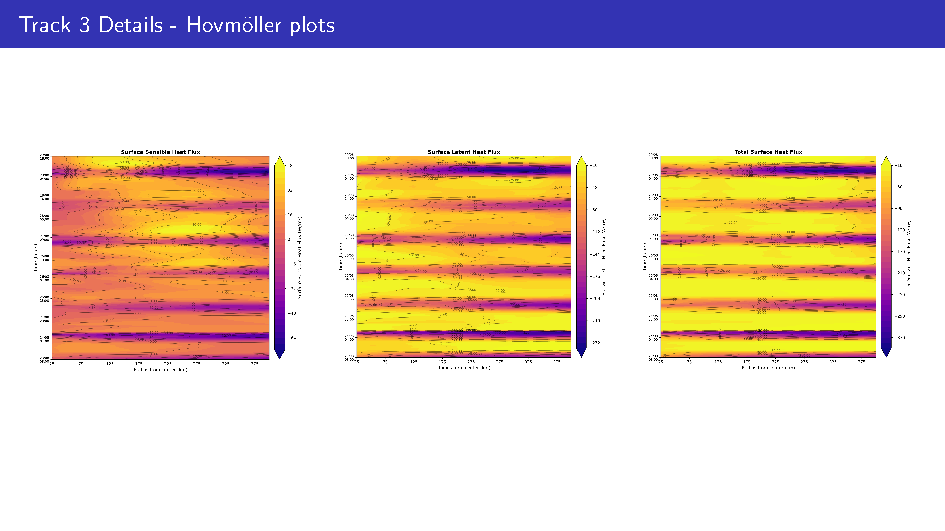
\includepdf[
    pages=-,
    scale=1,
    frame=true,
    % pagecommand={},
    pagecommand={\stepcounter{framenumber}},
    offset=0mm 0mm,       % Adjust position
    % templatesize={\textwidth}{\textheight} % Match template size
]{slides/hov-3.pdf}

\subsubsection{Track 3 \texttt{MODIS}}
\begin{frame}{\texttt{MODIS} Track 3 Visualization (2000m Scale)}
    \begin{center}
        \begin{figure}
            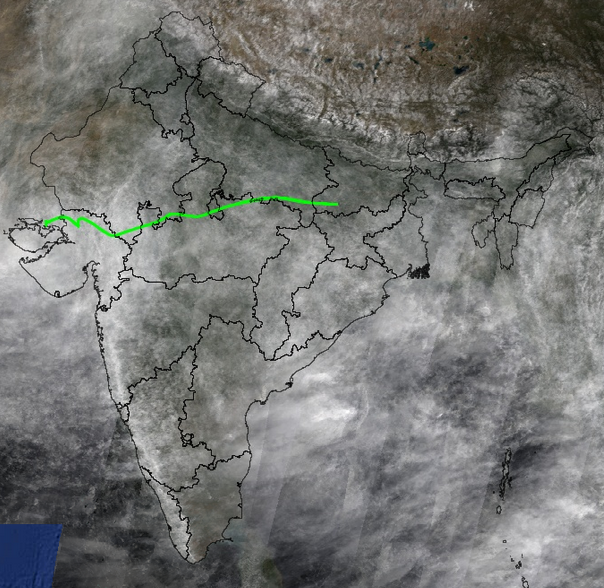
\includegraphics[width=0.45\linewidth]{images/MODIS-2024-Track_3.png}
        \end{figure}
        \label{fig:modistrack3}
    \end{center}

    % TODO:
    \vspace{0.2cm}
    {\tiny \textbf{Figure~\ref{fig:modistrack3} :} \texttt{MODIS} satellite image (true color) of Track. The characteristic depression cloud structure is visible with high Cloud cluster to the southwest of track. Image source: GEE, NASA \texttt{MODIS} Level 1B.}
    \vspace{0.1cm}
    {\tiny The 2nd cloud cluster region over BOB is genesis of Track 4}
\end{frame}

%%%%%%%%%%%%%%%% Track 4 %%%%%%%%%%%%%%
\subsection{Track 4}
\subsubsection{Track 4 Details}
\begin{frame}{Track 4 Details}
    \vspace{-0.1cm}
    \begin{center}
        \begin{columns}[T]
            \column{0.5\textwidth}
            \includegraphics[width=0.9\textwidth]{../version21-with-no-ocean-masking/output_2024/track_4/MD_track_4_detailed.png}

            % \vspace{0.05cm}
            % \footnotesize
            % \begin{block}{Statistics}
            %     \begin{itemize}
            %         \item Duration: 75 hours ($\sim$ 3 days)
            %         \item Category: short-lived MD
            %         \item \textbf{Origin:} Bay of Bengal (Oceanic)
            %     \end{itemize}
            % \end{block}

            \column{0.5\textwidth}
            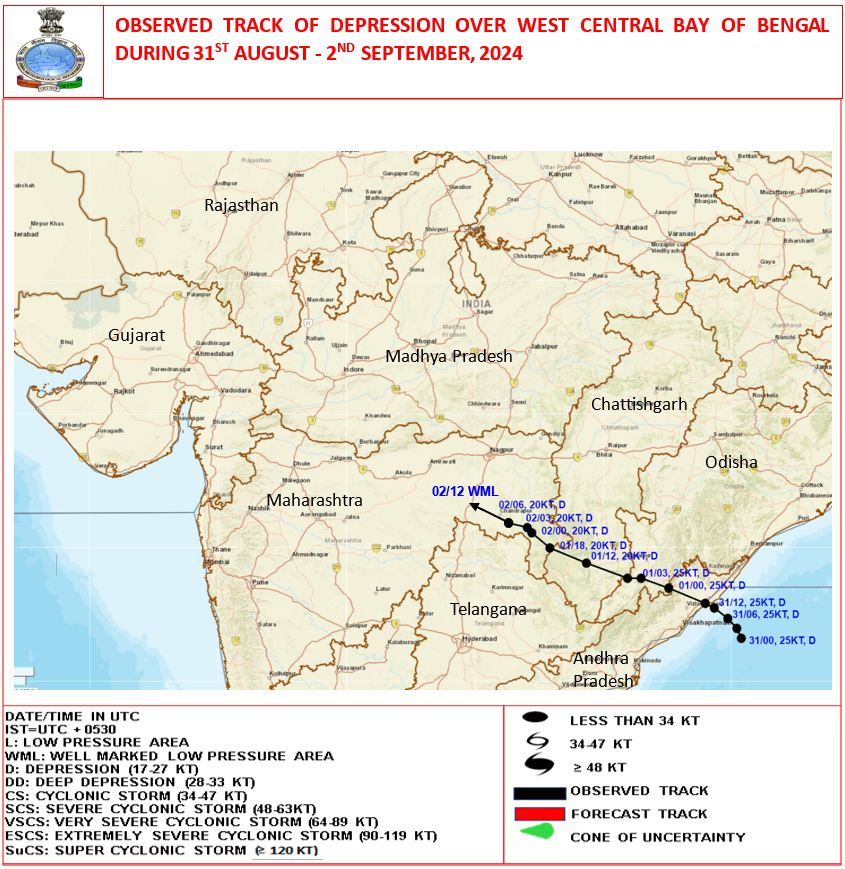
\includegraphics[width=0.8\textwidth]{images/August-31-Sep-02-2024.png}

            \footnote{\tiny Source RSMC New Delhi Report 2024 : \href{https://rsmcnewdelhi.imd.gov.in/report.php?internal_menu=MzQ=}{\url{https://rsmcnewdelhi.imd.gov.in/report.php?internal_menu=MzQ=}}}
        \end{columns}
    \end{center}
\end{frame}

\subsubsection{Track 4 Translation Speed}
\begin{frame}{Track 4 Translation speed of MD}
    \begin{center}
        \includegraphics[width=0.8\textwidth]{../version21-with-no-ocean-masking/output_2024/track_4/translational-speed/track_4_speed_ms.png}
    \end{center}
\end{frame}

\subsubsection{Track 4 HF Time evolution}
\begin{frame}{Track 4 Heat Flux evolution}
    \begin{center}
        \begin{figure}
            \includegraphics[width=0.6\textwidth]{../version21-with-no-ocean-masking/output_2024/track_4/time_series/track_4_heat_flux_time_series.png}
        \end{figure}
        \label{fig:track_4_heat_flux_timeseries}
    \end{center}

    \vspace{0.2cm}
    {\tiny \textbf{Figure~\ref{fig:track_4_heat_flux_timeseries} :} Time series of sensible, latent, and total heat fluxes for Track 4}% Note the dramatic increase in total heat flux upon landfall, primarily driven by latent heat component. This energy influx sustains the depression over land.}
\end{frame}

\subsubsection{Track 4 TP and SWVL1 Time evolution}
\begin{frame}{Track 4 \texttt{TP} and \texttt{SWVL1} Time evolution}
       \begin{figure}
           \centering
           \includegraphics[width=\textwidth]{../version21-with-no-ocean-masking/output_2024/track_4/time_series/track_4_TP-SWVL1_time_series.png}
       \end{figure}
       \label{fig:track_4_TP-SWVL1_time_series}

       % TODO:
       \vspace{0.2cm}
       {\tiny Figure~\ref{fig:track_4_TP-SWVL1_time_series} : Temporal evolution of \texttt{TP} and \texttt{SWVL1}. The vertical dashed line indicates landfall time} %([date/time])}. Key observation: [Variable] increases by X units upon landfall, supporting the hypothesis that [physical mechanism]. This pattern was consistent across all 6 depressions analyzed.}
\end{frame}

\subsubsection{Track 4 - Auto-Correlations}
\begin{frame}{Track 4 - \texttt{SWVL1} and \texttt{TP} Auto-Correlation}
    \begin{columns}[T]
        \begin{column}{0.5\textwidth}
            \begin{figure}
                \centering
                \includegraphics[width=\textwidth]{../version21-with-no-ocean-masking/output_2024/track_4/correlation_analysis/autocorrelation/track_4_autocorr_swvl1.png}
            \end{figure}
            \label{fig:track_4_SWVL1_autocorrelation}

            % TODO:
            \vspace{0.2cm}
            {\tiny \textbf{Figure~\ref{fig:track_4_SWVL1_autocorrelation} :}Auto-correlation of soil moisture (\texttt{SWVL1})  for Track 4.} % Maximum correlation of r = [X] occurs at lag [Y hours], suggesting that soil moisture response lags precipitation by approximately [Y hours]. This lag is consistent with water infiltration timescales in the region.}
        \end{column}

        \begin{column}{0.5\textwidth}
            \begin{figure}
                \centering
                \includegraphics[width=\textwidth]{../version21-with-no-ocean-masking/output_2024/track_4/correlation_analysis/autocorrelation/track_4_autocorr_tp.png}
            \end{figure}
            \label{fig:track_4_TP_autocorrelation}

            % TODO:
            \vspace{0.2cm}
            {\tiny \textbf{Figure~\ref{fig:track_4_TP_autocorrelation} :}Auto-correlation of Total precipitation (\texttt{TP}) for Track 4.} % Maximum correlation of r = [X] occurs at lag [Y hours], suggesting that soil moisture response lags precipitation by approximately [Y hours]. This lag is consistent with water infiltration timescales in the region.}
        \end{column}

        % \begin{column}{0.4\textwidth}
        %     \footnotesize
        %     \textbf{Summary:}
        %     \begin{itemize}
        %         \item The peak of correlation occurs at far left of zero-lag line (24 hours earlier).
        %         \item Antecedent moisture, Soil moisture levels are precursor to rainfall (or say sets condition for rainfall) events 24 hours later.
        %         \item Suggests very slow moving land-atmosphere feedback loop.
        %     \end{itemize}
        % \end{column}
    \end{columns}
\end{frame}

\begin{frame}{Track 3 - HF Auto-Correlation}
    \vspace{-0.3cm}
    \begin{columns}[T]
        \begin{column}{0.45\textwidth}
            \begin{figure}
                \centering
                \includegraphics[width=\textwidth]{../version21-with-no-ocean-masking/output_2024/track_4/correlation_analysis/autocorrelation/track_4_autocorr_latent_hf.png}
            \end{figure}
            \label{fig:track_4_LHF_autocorrelation}
        \end{column}

        \begin{column}{0.45\textwidth}
            \begin{figure}
                \centering
                \includegraphics[width=\textwidth]{../version21-with-no-ocean-masking/output_2024/track_4/correlation_analysis/autocorrelation/track_4_autocorr_sensible_hf.png}
            \end{figure}
            \label{fig:track_4_SHF_autocorrelation}
        \end{column}

        % \begin{column}{0.45\textwidth}
        %     \footnotesize
        %     \textbf{Summary:}
        %     \begin{itemize}
        %     \end{itemize}
        % \end{column}
    \end{columns}

    \vspace{-0.3cm}
    \begin{columns}[T]
        \begin{column}{0.45\textwidth}
            \begin{figure}
                \centering
                \includegraphics[width=\textwidth]{../version21-with-no-ocean-masking/output_2024/track_4/correlation_analysis/autocorrelation/track_4_autocorr_total_hf.png}
            \end{figure}
            \label{fig:track_4_THF_autocorrelation}
        \end{column}

        \begin{column}{0.45\textwidth}
            % TODO:
            \vspace{1.5cm}
            {\tiny \textbf{Figures :} Auto-correlation of Heat fluxes (\texttt{LHF, SHF} and \texttt{THF}) for Track 4.} % Maximum correlation of r = [X] occurs at lag [Y hours], suggesting that soil moisture response lags precipitation by approximately [Y hours]. This lag is consistent with water infiltration timescales in the region.}
        \end{column}
    \end{columns}
\end{frame}

\begin{frame}{Track 4 - \texttt{SWVL1-HF} Correlation}
    \vspace{-0.5cm}
    \begin{columns}[T]
        \begin{column}{0.8\textwidth}
            \begin{figure}
                \centering
                \includegraphics[width=\textwidth]{../version21-with-no-ocean-masking/output_2024/track_4/correlation_analysis/correlation/track_4_SWVL1-HF_correlation.png}
            \end{figure}
            \label{fig:track_4_swvl1-hf_correlation}

            \vspace{-0.4cm}
            \begin{figure}
                \centering
                \includegraphics[width=\textwidth]{../version21-with-no-ocean-masking/output_2024/track_4/correlation_analysis/correlation/track_4_TP-HF_correlation.png}
            \end{figure}
            \label{fig:track_4_tp-hf_correlation}
        \end{column}

        \begin{column}{0.2\textwidth}
        %     \footnotesize
        %     \textbf{Summary:}
        %     \begin{itemize}
        %         \item The peak of correlation occurs at far left of zero-lag line (24 hours earlier).
        %         \item Antecedent moisture, Soil moisture levels are precursor to rainfall (or say sets condition for rainfall) events 24 hours later.
        %         \item Suggests very slow moving land-atmosphere feedback loop.
        %     \end{itemize}
        \end{column}
    \end{columns}

    % \vspace{-0.3cm}
    % \begin{columns}[T]
    %     \begin{column}{0.45\textwidth}
    %
    %     \end{column}
    %
    %     \begin{column}{0.45\textwidth}
    %         % TODO:
    %         \vspace{1.5cm}
    %         {\tiny \textbf{Figures :} Correlation for Track 4.} % Maximum correlation of r = [X] occurs at lag [Y hours], suggesting that soil moisture response lags precipitation by approximately [Y hours]. This lag is consistent with water infiltration timescales in the region.}
    %     \end{column}
    % \end{columns}
\end{frame}

\subsubsection{Track 4 TP-SWVL1 Correlation}
\begin{frame}{Track 4 \texttt{TP-SWVL1} Correlation}
    \begin{columns}[T]
        \begin{column}{0.6\textwidth}
            \begin{figure}
                \centering
                \includegraphics[width=\textwidth]{../version21-with-no-ocean-masking/output_2024/track_4/correlation_analysis/correlation/track_4_TP-SWVL1_correlation.png}
            \end{figure}
            \label{fig:track_4_tp-swvl1_correlation}
        \end{column}

        \begin{column}{0.4\textwidth}
            \footnotesize
        %     \textbf{Statistical Summary :}
        %     \begin{itemize}
        %         \item \textbf{Pearson r :} \texttt{-0.2633} – Weak negative linear relationship between precipitation and soil moisture more rainfall leads lower soil moisture (why? 1. maybe because track is short-lived, 2. MD doesn't penetrate inland deep). \cite{kishtawal2013enhancement} 
        %         \item \textbf{Spearman $\rho$ :} \texttt{-0.2930} – slight negative monotonic trend suggests higher rain corresponds to lower simultaneous soil moisture.
        %         \item \textbf{p-value :} \texttt{3.0054 \times 10$^{-2}$} – Statistically significant ($p < 0.05$), though the correlation strength is low.
        %         \item \textbf{Mean TP :} 0.49 $mm/hr$
        %         \item \textbf{Mean SM :} 0.14 m$^3$/m$^3$
        %     \end{itemize}
        \end{column}
    \end{columns}
\end{frame}

\begin{frame}{Track 4 - \texttt{TP-SWVL1} Lag Correlation}
    \begin{columns}[T]
        \begin{column}{0.6\textwidth}
            \begin{figure}
                \centering
                \includegraphics[width=\textwidth]{../version21-with-no-ocean-masking/output_2024/track_4/correlation_analysis/lag_correlation/track_4_TP-SWVL1_lag_correlation.png}
            \end{figure}
            \label{fig:track_4_TP-SWVL1_lag_correlation}

            % TODO:
            \vspace{0.2cm}
            {\tiny \textbf{Figure~\ref{fig:track_4_TP-SWVL1_lag_correlation} :}Lag correlation between precipitation (\texttt{TP}) and soil moisture (\texttt{SWVL1}) for Track 4.} % Maximum correlation of r = [X] occurs at lag [Y hours], suggesting that soil moisture response lags precipitation by approximately [Y hours]. This lag is consistent with water infiltration timescales in the region.}
        \end{column}

        % \begin{column}{0.4\textwidth}
        %     \footnotesize
        %     \textbf{Summary:}
        %     \begin{itemize}
        %         \item The peak of correlation occurs at far left of zero-lag line (24 hours earlier).
        %         \item Antecedent moisture, Soil moisture levels are precursor to rainfall (or say sets condition for rainfall) events 24 hours later.
        %         \item Suggests very slow moving land-atmosphere feedback loop.
        %     \end{itemize}
        % \end{column}
    \end{columns}
\end{frame}

\begin{frame}{Track 4 \texttt{SWVL1-HF} Lag Correlation}
    \begin{columns}[t]
        \begin{column}{0.5\textwidth}
            \begin{center}
                \includegraphics[width=0.9\textwidth]{../version21-with-no-ocean-masking/output_2024/track_4/correlation_analysis/lag_correlation/track_4_SWVL1-LHF_lag_correlation.png} \\
                \includegraphics[width=0.9\textwidth]{../version21-with-no-ocean-masking/output_2024/track_4/correlation_analysis/lag_correlation/track_4_SWVL1-SHF_lag_correlation.png}
            \end{center}
        \end{column}

        \begin{column}{0.5\textwidth}
            \begin{center}
                \includegraphics[width=0.9\textwidth]{../version21-with-no-ocean-masking/output_2024/track_4/correlation_analysis/lag_correlation/track_4_SWVL1-THF_lag_correlation.png}
            \end{center}
        \end{column}
    \end{columns}
\end{frame}

\begin{frame}{Track 4 \texttt{TP-HF} Lag Correlation}
    \begin{columns}[t]
        \begin{column}{0.5\textwidth}
            \begin{center}
                \includegraphics[width=0.9\textwidth]{../version21-with-no-ocean-masking/output_2024/track_4/correlation_analysis/lag_correlation/track_4_TP-LHF_lag_correlation.png} \\
                \includegraphics[width=0.9\textwidth]{../version21-with-no-ocean-masking/output_2024/track_4/correlation_analysis/lag_correlation/track_4_TP-SHF_lag_correlation.png}
            \end{center}
        \end{column}

        \begin{column}{0.5\textwidth}
            \begin{center}
                \includegraphics[width=0.9\textwidth]{../version21-with-no-ocean-masking/output_2024/track_4/correlation_analysis/lag_correlation/track_4_TP-THF_lag_correlation.png}
            \end{center}
        \end{column}
    \end{columns}
\end{frame}

\subsubsection{Track 4 Hovm\"oller plots}
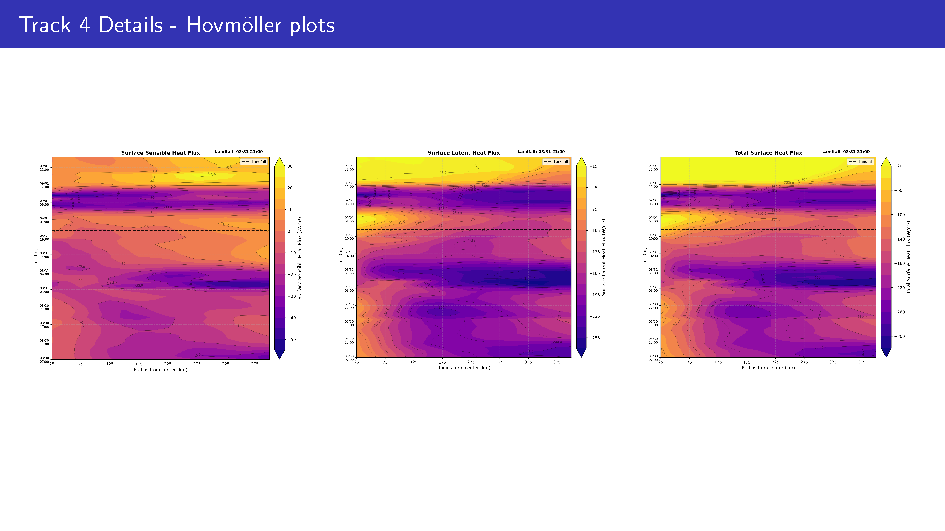
\includepdf[
    pages=-,
    scale=1,
    frame=true,
    % pagecommand={},
    pagecommand={\stepcounter{framenumber}},
    offset=0mm 0mm,       % Adjust position
    % templatesize={\textwidth}{\textheight} % Match template size
]{slides/hov-4.pdf}

% TODO: Physical reality
%    Track 4 has a very short duration (59 hours) and a low mean soil moisture (0.178). The negative value likely indicates:
%     - Fast Dry-down: The system experienced a burst of precipitation that spiked soil moisture, but because the soil was dry or had low retention capacity, that moisture evaporated or drained so rapidly that by the 24-hour mark, the soil was "drier than average."
%     - Diurnal Dominance over Trend: In short-lived tracks, if the diurnal cycle (daytime evaporation vs. nighttime stability) is stronger than the overall moisture trend, the ACF can dip into negative territory at specific lags as the "day" state is the opposite of the "night" state.

\subsubsection{Track 4 \texttt{MODIS}}
\begin{frame}{\texttt{MODIS} Track 4 Visualization (2000m Scale)}
    \begin{center}
        \begin{figure}
            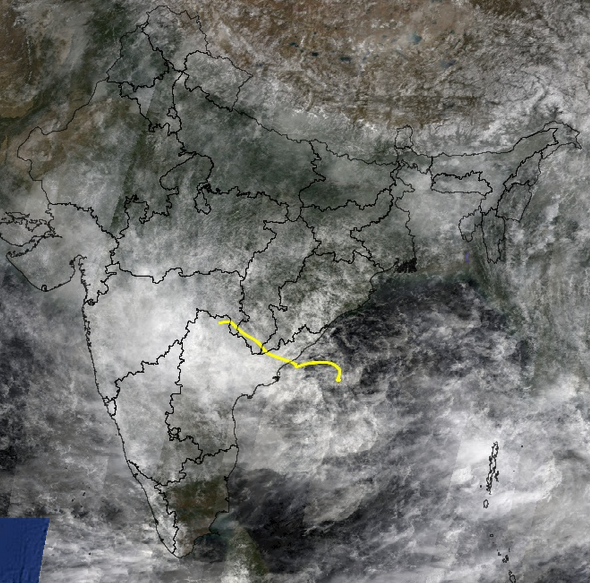
\includegraphics[width=0.45\linewidth]{images/MODIS-2024-Track_4.png}
        \end{figure}
        \label{fig:modistrack4}
    \end{center}

    % TODO:
    \vspace{0.2cm}
    {\tiny \textbf{Figure~\ref{fig:modistrack4} :} \texttt{MODIS} satellite image of Track 4. The characteristic depression cloud structure is visible with high Cloud cluster to the southwest of track. Image source: GEE, NASA \texttt{MODIS} Level 1B.}
\end{frame}

%%%%%%%%%%%%%%%% Track 5 %%%%%%%%%%%%%%
\subsection{Track 5}
\subsubsection{Track 5 Details}
\begin{frame}{Track 5 Details}
    \vspace{-0.19cm}
    \begin{center}
        \begin{columns}[T]
            \column{0.53\textwidth}
            \includegraphics[width=0.75\textwidth]{../version21-with-no-ocean-masking/output_2024/track_5/MD_track_5_detailed.png}

            % \vspace{0.01cm}
            % \footnotesize
            % \begin{block}{Statistics}
            %     \begin{itemize}
            %         \item Duration: 165 hours ($\sim$ 7 days)
            %         \item Category: long-lived MD \vspace{-0.03cm}
            %         \item \textbf{Origin:} Bay of Bengal (Oceanic)  \vspace{-0.03cm}
            %     \end{itemize}
            % \end{block}

            \column{0.47\textwidth}
            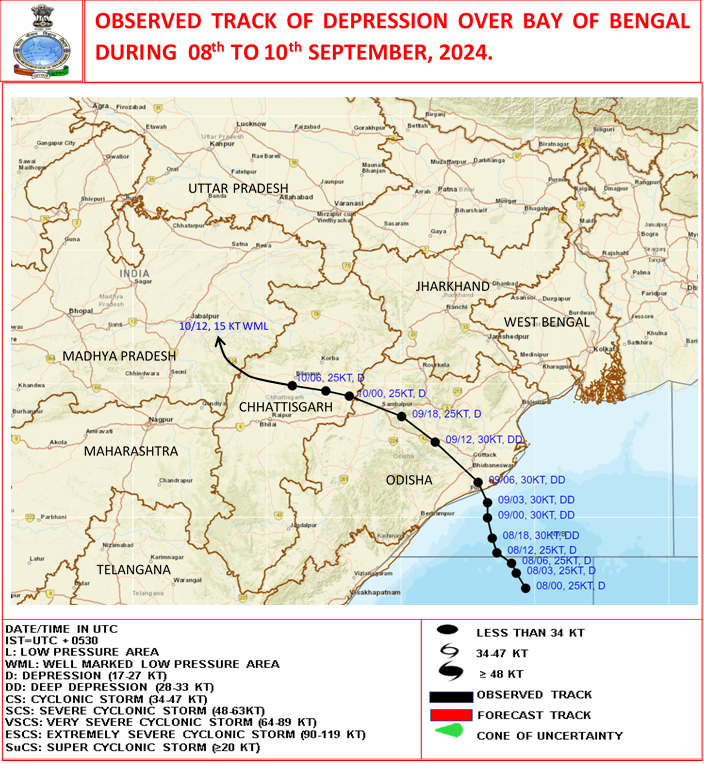
\includegraphics[width=0.8\textwidth]{images/September-08-10-2024.png}

            \footnotesize RSMC New Delhi Track\footnotemark[1]

            \footnotetext{\tiny Source  RSMC New Delhi Report 2024 : \href{https://rsmcnewdelhi.imd.gov.in/report.php?internal_menu=MzQ=}{\url{https://rsmcnewdelhi.imd.gov.in/report.php?internal_menu=MzQ=}}}
        \end{columns}

        \vspace{-0.26cm}
        \tiny
        \begin{alertblock}{\tiny Discrepancy}
            The detected track extends further north-west, a period of weakened vorticity signal and reduction in MD centre transition speed (from 5 to 1 m/s) during the land phase on \textbf{September 10th}. Main reason could be MD encounter elevated region of \textbf{Eastern Ghats}.
            RSMC New Delhi ignores/truncate the track after this weakening while IMD reported increase in vorticity after some period (September 11th) thus considering longer inland MD track (till Sept 13th). (I will be taking IMD report as preferred source.)
        \end{alertblock}
    \end{center}
\end{frame}

\subsubsection{Track 5 Translation Speed}
\begin{frame}{Track 5 Translation speed of MD}
    \begin{center}
        \includegraphics[width=0.8\textwidth]{../version21-with-no-ocean-masking/output_2024/track_5/translational-speed/track_5_speed_ms.png}
    \end{center}
\end{frame}

\subsubsection{Track 5 HF Time evolution}
\begin{frame}{Track 5 Heat Flux evolution}
    \begin{center}
        \begin{figure}
            \includegraphics[width=0.6\textwidth]{../version21-with-no-ocean-masking/output_2024/track_5/time_series/track_5_heat_flux_time_series.png}
        \end{figure}
        \label{fig:track_5_heat_flux_timeseries}
    \end{center}

    \vspace{0.2cm}
    {\tiny \textbf{Figure~\ref{fig:track_5_heat_flux_timeseries} :} Time series of sensible, latent, and total heat fluxes for Track 5}% Note the dramatic increase in total heat flux upon landfall, primarily driven by latent heat component. This energy influx sustains the depression over land.}
\end{frame}

\subsubsection{Track 5 TP and SWVL1 Time evolution}
\begin{frame}{Track 5 \texttt{TP} and \texttt{SWVL1} Time evolution}
       \begin{figure}
           \centering
           \includegraphics[width=\textwidth]{../version21-with-no-ocean-masking/output_2024/track_5/time_series/track_5_TP-SWVL1_time_series.png}
       \end{figure}
       \label{fig:track_5_TP-SWVL1_time_series}

       % TODO:
       \vspace{0.2cm}
       {\tiny Figure~\ref{fig:track_5_TP-SWVL1_time_series} : Temporal evolution of \texttt{TP} and \texttt{SWVL1}. The vertical dashed line indicates landfall time} %([date/time])}. Key observation: [Variable] increases by X units upon landfall, supporting the hypothesis that [physical mechanism]. This pattern was consistent across all 6 depressions analyzed.}
\end{frame}

\subsubsection{Track 5 - Auto-Correlations}
\begin{frame}{Track 5 - \texttt{SWVL1} and \texttt{TP} Auto-Correlation}
    \begin{columns}[T]
        \begin{column}{0.5\textwidth}
            \begin{figure}
                \centering
                \includegraphics[width=\textwidth]{../version21-with-no-ocean-masking/output_2024/track_5/correlation_analysis/autocorrelation/track_5_autocorr_swvl1.png}
            \end{figure}
            \label{fig:track_5_SWVL1_autocorrelation}

            % TODO:
            \vspace{0.2cm}
            {\tiny \textbf{Figure~\ref{fig:track_5_SWVL1_autocorrelation} :}Auto-correlation of soil moisture (\texttt{SWVL1}) for Track 5.} % Maximum correlation of r = [X] occurs at lag [Y hours], suggesting that soil moisture response lags precipitation by approximately [Y hours]. This lag is consistent with water infiltration timescales in the region.}
        \end{column}

        \begin{column}{0.5\textwidth}
            \begin{figure}
                \centering
                \includegraphics[width=\textwidth]{../version21-with-no-ocean-masking/output_2024/track_5/correlation_analysis/autocorrelation/track_5_autocorr_tp.png}
            \end{figure}
            \label{fig:track_5_TP_autocorrelation}

            % TODO:
            \vspace{0.2cm}
            {\tiny \textbf{Figure~\ref{fig:track_5_TP_autocorrelation} :}Auto-correlation of Total precipitation (\texttt{TP}) for Track 5.} % Maximum correlation of r = [X] occurs at lag [Y hours], suggesting that soil moisture response lags precipitation by approximately [Y hours]. This lag is consistent with water infiltration timescales in the region.}
        \end{column}

        % \begin{column}{0.4\textwidth}
        %     \footnotesize
        %     \textbf{Summary:}
        %     \begin{itemize}
        %         \item The peak of correlation occurs at far left of zero-lag line (24 hours earlier).
        %         \item Antecedent moisture, Soil moisture levels are precursor to rainfall (or say sets condition for rainfall) events 24 hours later.
        %         \item Suggests very slow moving land-atmosphere feedback loop.
        %     \end{itemize}
        % \end{column}
    \end{columns}
\end{frame}

\begin{frame}{Track 5 - HF Auto-Correlation}
    \vspace{-0.3cm}
    \begin{columns}[T]
        \begin{column}{0.45\textwidth}
            \begin{figure}
                \centering
                \includegraphics[width=\textwidth]{../version21-with-no-ocean-masking/output_2024/track_5/correlation_analysis/autocorrelation/track_5_autocorr_latent_hf.png}
            \end{figure}
            \label{fig:track_5_LHF_autocorrelation}
        \end{column}

        \begin{column}{0.45\textwidth}
            \begin{figure}
                \centering
                \includegraphics[width=\textwidth]{../version21-with-no-ocean-masking/output_2024/track_5/correlation_analysis/autocorrelation/track_5_autocorr_sensible_hf.png}
            \end{figure}
            \label{fig:track_5_SHF_autocorrelation}
        \end{column}

        % \begin{column}{0.45\textwidth}
        %     \footnotesize
        %     \textbf{Summary:}
        %     \begin{itemize}
        %     \end{itemize}
        % \end{column}
    \end{columns}

    \vspace{-0.3cm}
    \begin{columns}[T]
        \begin{column}{0.45\textwidth}
            \begin{figure}
                \centering
                \includegraphics[width=\textwidth]{../version21-with-no-ocean-masking/output_2024/track_5/correlation_analysis/autocorrelation/track_5_autocorr_total_hf.png}
            \end{figure}
            \label{fig:track_5_THF_autocorrelation}
        \end{column}

        \begin{column}{0.45\textwidth}
            % TODO:
            \vspace{1.5cm}
            {\tiny \textbf{Figures :} Auto-correlation of Heat fluxes (\texttt{LHF, SHF} and \texttt{THF}) for Track 5.} % Maximum correlation of r = [X] occurs at lag [Y hours], suggesting that soil moisture response lags precipitation by approximately [Y hours]. This lag is consistent with water infiltration timescales in the region.}
        \end{column}
    \end{columns}
\end{frame}

\begin{frame}{Track 5 - \texttt{SWVL1-HF} Correlation}
    \vspace{-0.5cm}
    \begin{columns}[T]
        \begin{column}{0.8\textwidth}
            \begin{figure}
                \centering
                \includegraphics[width=\textwidth]{../version21-with-no-ocean-masking/output_2024/track_5/correlation_analysis/correlation/track_5_SWVL1-HF_correlation.png}
            \end{figure}
            \label{fig:track_5_swvl1-hf_correlation}

            \vspace{-0.4cm}
            \begin{figure}
                \centering
                \includegraphics[width=\textwidth]{../version21-with-no-ocean-masking/output_2024/track_5/correlation_analysis/correlation/track_5_TP-HF_correlation.png}
            \end{figure}
            \label{fig:track_5_tp-hf_correlation}
        \end{column}

        \begin{column}{0.2\textwidth}
        %     \footnotesize
        %     \textbf{Summary:}
        %     \begin{itemize}
        %         \item The peak of correlation occurs at far left of zero-lag line (24 hours earlier).
        %         \item Antecedent moisture, Soil moisture levels are precursor to rainfall (or say sets condition for rainfall) events 24 hours later.
        %         \item Suggests very slow moving land-atmosphere feedback loop.
        %     \end{itemize}
        \end{column}
    \end{columns}

    % \vspace{-0.3cm}
    % \begin{columns}[T]
    %     \begin{column}{0.45\textwidth}
    %
    %     \end{column}
    %
    %     \begin{column}{0.45\textwidth}
    %         % TODO:
    %         \vspace{1.5cm}
    %         {\tiny \textbf{Figures :} Correlation for Track 2.} % Maximum correlation of r = [X] occurs at lag [Y hours], suggesting that soil moisture response lags precipitation by approximately [Y hours]. This lag is consistent with water infiltration timescales in the region.}
    %     \end{column}
    % \end{columns}
\end{frame}

\subsubsection{Track 5 TP-SWVL1 Correlation}
\begin{frame}{Track 5 \texttt{TP-SWVL1} Correlation}
    \begin{columns}[T]
        \begin{column}{0.6\textwidth}
            \begin{figure}
                \centering
                \includegraphics[width=\textwidth]{../version21-with-no-ocean-masking/output_2024/track_5/correlation_analysis/correlation/track_5_TP-SWVL1_correlation.png}
            \end{figure}
            \label{fig:track_5_tp-swvl1_correlation}
        \end{column}

        \begin{column}{0.4\textwidth}
            \footnotesize
        %     \textbf{Statistical Summary :}
        %     \begin{itemize}
        %         \item \textbf{Pearson r :} \texttt{-0.2633} – Weak negative linear relationship between precipitation and soil moisture more rainfall leads lower soil moisture (why? 1. maybe because track is short-lived, 2. MD doesn't penetrate inland deep). \cite{kishtawal2013enhancement} 
        %         \item \textbf{Spearman $\rho$ :} \texttt{-0.2930} – slight negative monotonic trend suggests higher rain corresponds to lower simultaneous soil moisture.
        %         \item \textbf{p-value :} \texttt{3.0054 \times 10$^{-2}$} – Statistically significant ($p < 0.05$), though the correlation strength is low.
        %         \item \textbf{Mean TP :} 0.49 $mm/hr$
        %         \item \textbf{Mean SM :} 0.14 m$^3$/m$^3$
        %     \end{itemize}
        \end{column}
    \end{columns}
\end{frame}

\begin{frame}{Track 5 - \texttt{TP-SWVL1} Lag Correlation}
    \begin{columns}[T]
        \begin{column}{0.6\textwidth}
            \begin{figure}
                \centering
                \includegraphics[width=\textwidth]{../version21-with-no-ocean-masking/output_2024/track_5/correlation_analysis/lag_correlation/track_5_TP-SWVL1_lag_correlation.png}
            \end{figure}
            \label{fig:track_5_TP-SWVL1_lag_correlation}

            % TODO:
            \vspace{0.2cm}
            {\tiny \textbf{Figure~\ref{fig:track_5_TP-SWVL1_lag_correlation} :}Lag correlation between precipitation (\texttt{TP}) and soil moisture (\texttt{SWVL1}) for Track 5.} % Maximum correlation of r = [X] occurs at lag [Y hours], suggesting that soil moisture response lags precipitation by approximately [Y hours]. This lag is consistent with water infiltration timescales in the region.}
        \end{column}

        % \begin{column}{0.4\textwidth}
        %     \footnotesize
        %     \textbf{Summary:}
        %     \begin{itemize}
        %         \item The peak of correlation occurs at far left of zero-lag line (24 hours earlier).
        %         \item Antecedent moisture, Soil moisture levels are precursor to rainfall (or say sets condition for rainfall) events 24 hours later.
        %         \item Suggests very slow moving land-atmosphere feedback loop.
        %     \end{itemize}
        % \end{column}
    \end{columns}
\end{frame}

\begin{frame}{Track 5 \texttt{SWVL1-HF} Lag Correlation}
    \begin{columns}[t]
        \begin{column}{0.5\textwidth}
            \begin{center}
                \includegraphics[width=0.9\textwidth]{../version21-with-no-ocean-masking/output_2024/track_5/correlation_analysis/lag_correlation/track_5_SWVL1-LHF_lag_correlation.png} \\
                \includegraphics[width=0.9\textwidth]{../version21-with-no-ocean-masking/output_2024/track_5/correlation_analysis/lag_correlation/track_5_SWVL1-SHF_lag_correlation.png}
            \end{center}
        \end{column}

        \begin{column}{0.5\textwidth}
            \begin{center}
                \includegraphics[width=0.9\textwidth]{../version21-with-no-ocean-masking/output_2024/track_5/correlation_analysis/lag_correlation/track_5_SWVL1-THF_lag_correlation.png}
            \end{center}
        \end{column}
    \end{columns}
\end{frame}

\begin{frame}{Track 5 \texttt{TP-HF} Lag Correlation}
    \begin{columns}[t]
        \begin{column}{0.5\textwidth}
            \begin{center}
                \includegraphics[width=0.9\textwidth]{../version21-with-no-ocean-masking/output_2024/track_5/correlation_analysis/lag_correlation/track_5_TP-LHF_lag_correlation.png} \\
                \includegraphics[width=0.9\textwidth]{../version21-with-no-ocean-masking/output_2024/track_5/correlation_analysis/lag_correlation/track_5_TP-SHF_lag_correlation.png}
            \end{center}
        \end{column}

        \begin{column}{0.5\textwidth}
            \begin{center}
                \includegraphics[width=0.9\textwidth]{../version21-with-no-ocean-masking/output_2024/track_5/correlation_analysis/lag_correlation/track_5_TP-THF_lag_correlation.png}
            \end{center}
        \end{column}
    \end{columns}
\end{frame}

\subsubsection{Track 5 Hovm\"oller plots}
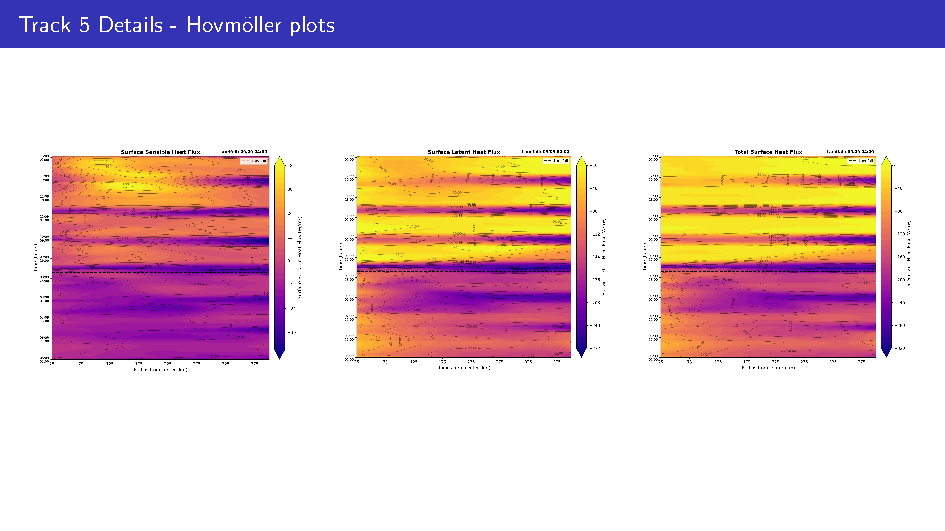
\includepdf[
    pages=-,
    scale=1,
    frame=true,
    % pagecommand={},
    pagecommand={\stepcounter{framenumber}},
    offset=0mm 0mm,       % Adjust position
    % templatesize={\textwidth}{\textheight} % Match template size
]{slides/hov-5.pdf}

\subsubsection{Track 5 \texttt{MODIS}}
\begin{frame}{\texttt{MODIS} Track 5 Visualization (2000m Scale)}
    \begin{center}
        \begin{figure}
            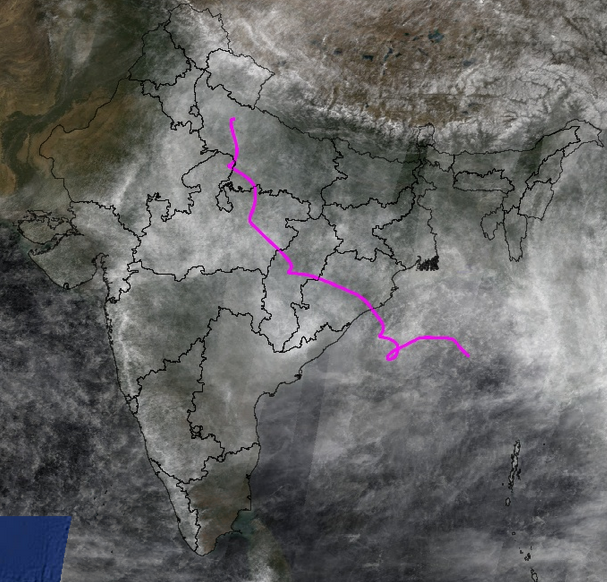
\includegraphics[width=0.45\linewidth]{images/MODIS-2024-Track_5.png}
        \end{figure}
        \label{fig:modistrack5}
    \end{center}

    % TODO:
    \vspace{0.2cm}
    {\tiny \textbf{Figure~\ref{fig:modistrack5} :} \texttt{MODIS} satellite image (true color) of Track. The characteristic depression cloud structure is visible with high Cloud cluster to the southwest of track. Image source: GEE, NASA \texttt{MODIS} Level 1B.}
\end{frame}

%%%%%%%%%%%%%%%% Track 6 %%%%%%%%%%%%%%
\subsection{Track 6}
\subsubsection{Track 6 Details}
\begin{frame}{Track 6 Details}
    \vspace{-0.1cm}
    \begin{center}
        \begin{columns}[T]
            \column{0.5\textwidth}
            \includegraphics[width=0.9\textwidth]{../version21-with-no-ocean-masking/output_2024/track_6/MD_track_6_detailed.png}

            \vspace{0.05cm}
            \footnotesize
            \begin{block}{Statistics}
                \begin{itemize}
                    \item Duration: 117 hours ($\sim$ 5 days)
                    \item Category: long-lived MD
                    \item Originated: over land
                \end{itemize}
            \end{block}

            \column{0.5\textwidth}
            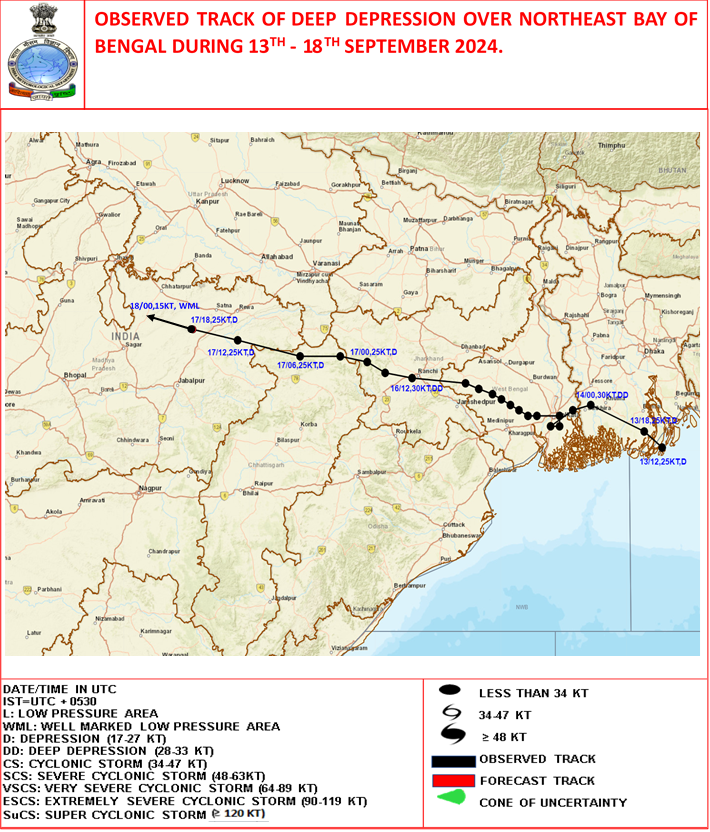
\includegraphics[width=0.8\textwidth]{images/September-13-18-2024.png}

            \footnotetext{\tiny Source  RSMC New Delhi Report 2024 : \href{https://rsmcnewdelhi.imd.gov.in/report.php?internal_menu=MzQ=}{\url{https://rsmcnewdelhi.imd.gov.in/report.php?internal_menu=MzQ=}}}
        \end{columns}
    \end{center}
\end{frame}

\subsubsection{Track 6 Translation Speed}
\begin{frame}{Track 6 Translation speed of MD}
    \begin{center}
        \includegraphics[width=0.8\textwidth]{../version21-with-no-ocean-masking/output_2024/track_6/translational-speed/track_6_speed_ms.png}
    \end{center}
\end{frame}

\subsubsection{Track 6 HF Time evolution}
\begin{frame}{Track 6 Heat Flux evolution}
    \begin{center}
        \begin{figure}
            \includegraphics[width=0.6\textwidth]{../version21-with-no-ocean-masking/output_2024/track_6/time_series/track_6_heat_flux_time_series.png}
        \end{figure}
        \label{fig:track_6_heat_flux_timeseries}
    \end{center}

    \vspace{0.2cm}
    {\tiny \textbf{Figure~\ref{fig:track_6_heat_flux_timeseries} :} Time series of sensible, latent, and total heat fluxes for Track 6}% Note the dramatic increase in total heat flux upon landfall, primarily driven by latent heat component. This energy influx sustains the depression over land.}
\end{frame}

\subsubsection{Track 6 TP and SWVL1 Time evolution}
\begin{frame}{Track 6 \texttt{TP} and \texttt{SWVL1} Time evolution}
       \begin{figure}
           \centering
           \includegraphics[width=\textwidth]{../version21-with-no-ocean-masking/output_2024/track_6/time_series/track_6_TP-SWVL1_time_series.png}
       \end{figure}
       \label{fig:track_6_TP-SWVL1_time_series}

       % TODO:
       \vspace{0.2cm}
       {\tiny Figure~\ref{fig:track_6_TP-SWVL1_time_series} : Temporal evolution of \texttt{TP} and \texttt{SWVL1}. The vertical dashed line indicates landfall time} %([date/time])}. Key observation: [Variable] increases by X units upon landfall, supporting the hypothesis that [physical mechanism]. This pattern was consistent across all 6 depressions analyzed.}
\end{frame}

\subsubsection{Track 6 - Auto-Correlations}
\begin{frame}{Track 6 - \texttt{SWVL1} and \texttt{TP} Auto-Correlation}
    \begin{columns}[T]
        \begin{column}{0.5\textwidth}
            \begin{figure}
                \centering
                \includegraphics[width=\textwidth]{../version21-with-no-ocean-masking/output_2024/track_6/correlation_analysis/autocorrelation/track_6_autocorr_swvl1.png}
            \end{figure}
            \label{fig:track_6_SWVL1_autocorrelation}

            % TODO:
            \vspace{0.2cm}
            {\tiny \textbf{Figure~\ref{fig:track_6_SWVL1_autocorrelation} :}Auto-correlation of soil moisture (\texttt{SWVL1}) for Track 6.} % Maximum correlation of r = [X] occurs at lag [Y hours], suggesting that soil moisture response lags precipitation by approximately [Y hours]. This lag is consistent with water infiltration timescales in the region.}
        \end{column}

        \begin{column}{0.5\textwidth}
            \begin{figure}
                \centering
                \includegraphics[width=\textwidth]{../version21-with-no-ocean-masking/output_2024/track_6/correlation_analysis/autocorrelation/track_6_autocorr_tp.png}
            \end{figure}
            \label{fig:track_6_TP_autocorrelation}

            % TODO:
            \vspace{0.2cm}
            {\tiny \textbf{Figure~\ref{fig:track_6_TP_autocorrelation} :}Auto-correlation of Total precipitation (\texttt{TP}) for Track 6.} % Maximum correlation of r = [X] occurs at lag [Y hours], suggesting that soil moisture response lags precipitation by approximately [Y hours]. This lag is consistent with water infiltration timescales in the region.}
        \end{column}

        % \begin{column}{0.4\textwidth}
        %     \footnotesize
        %     \textbf{Summary:}
        %     \begin{itemize}
        %         \item The peak of correlation occurs at far left of zero-lag line (24 hours earlier).
        %         \item Antecedent moisture, Soil moisture levels are precursor to rainfall (or say sets condition for rainfall) events 24 hours later.
        %         \item Suggests very slow moving land-atmosphere feedback loop.
        %     \end{itemize}
        % \end{column}
    \end{columns}
\end{frame}

\begin{frame}{Track 6 - HF Auto-Correlation}
    \vspace{-0.3cm}
    \begin{columns}[T]
        \begin{column}{0.45\textwidth}
            \begin{figure}
                \centering
                \includegraphics[width=\textwidth]{../version21-with-no-ocean-masking/output_2024/track_6/correlation_analysis/autocorrelation/track_6_autocorr_latent_hf.png}
            \end{figure}
            \label{fig:track_6_LHF_autocorrelation}
        \end{column}

        \begin{column}{0.45\textwidth}
            \begin{figure}
                \centering
                \includegraphics[width=\textwidth]{../version21-with-no-ocean-masking/output_2024/track_6/correlation_analysis/autocorrelation/track_6_autocorr_sensible_hf.png}
            \end{figure}
            \label{fig:track_6_SHF_autocorrelation}
        \end{column}

        % \begin{column}{0.45\textwidth}
        %     \footnotesize
        %     \textbf{Summary:}
        %     \begin{itemize}
        %     \end{itemize}
        % \end{column}
    \end{columns}

    \vspace{-0.3cm}
    \begin{columns}[T]
        \begin{column}{0.45\textwidth}
            \begin{figure}
                \centering
                \includegraphics[width=\textwidth]{../version21-with-no-ocean-masking/output_2024/track_6/correlation_analysis/autocorrelation/track_6_autocorr_total_hf.png}
            \end{figure}
            \label{fig:track_6_THF_autocorrelation}
        \end{column}

        \begin{column}{0.45\textwidth}
            % TODO:
            \vspace{1.5cm}
            {\tiny \textbf{Figures :} Auto-correlation of Heat fluxes (\texttt{LHF, SHF} and \texttt{THF}) for Track 6.} % Maximum correlation of r = [X] occurs at lag [Y hours], suggesting that soil moisture response lags precipitation by approximately [Y hours]. This lag is consistent with water infiltration timescales in the region.}
        \end{column}
    \end{columns}
\end{frame}

\begin{frame}{Track 6 - \texttt{SWVL1-HF} Correlation}
    \vspace{-0.5cm}
    \begin{columns}[T]
        \begin{column}{0.8\textwidth}
            \begin{figure}
                \centering
                \includegraphics[width=\textwidth]{../version21-with-no-ocean-masking/output_2024/track_5/correlation_analysis/correlation/track_5_SWVL1-HF_correlation.png}
            \end{figure}
            \label{fig:track_5_swvl1-hf_correlation}

            \vspace{-0.4cm}
            \begin{figure}
                \centering
                \includegraphics[width=\textwidth]{../version21-with-no-ocean-masking/output_2024/track_5/correlation_analysis/correlation/track_5_TP-HF_correlation.png}
            \end{figure}
            \label{fig:track_5_tp-hf_correlation}
        \end{column}

        \begin{column}{0.2\textwidth}
        %     \footnotesize
        %     \textbf{Summary:}
        %     \begin{itemize}
        %         \item The peak of correlation occurs at far left of zero-lag line (24 hours earlier).
        %         \item Antecedent moisture, Soil moisture levels are precursor to rainfall (or say sets condition for rainfall) events 24 hours later.
        %         \item Suggests very slow moving land-atmosphere feedback loop.
        %     \end{itemize}
        \end{column}
    \end{columns}

    % \vspace{-0.3cm}
    % \begin{columns}[T]
    %     \begin{column}{0.45\textwidth}
    %
    %     \end{column}
    %
    %     \begin{column}{0.45\textwidth}
    %         % TODO:
    %         \vspace{1.5cm}
    %         {\tiny \textbf{Figures :} Correlation for Track 2.} % Maximum correlation of r = [X] occurs at lag [Y hours], suggesting that soil moisture response lags precipitation by approximately [Y hours]. This lag is consistent with water infiltration timescales in the region.}
    %     \end{column}
    % \end{columns}
\end{frame}

\subsubsection{Track 5 TP-SWVL1 Correlation}
\begin{frame}{Track 5 \texttt{TP-SWVL1} Correlation}
    \begin{columns}[T]
        \begin{column}{0.6\textwidth}
            \begin{figure}
                \centering
                \includegraphics[width=\textwidth]{../version21-with-no-ocean-masking/output_2024/track_6/correlation_analysis/correlation/track_6_TP-SWVL1_correlation.png}
            \end{figure}
            \label{fig:track_6_tp-swvl1_correlation}
        \end{column}

        \begin{column}{0.4\textwidth}
            \footnotesize
        %     \textbf{Statistical Summary :}
        %     \begin{itemize}
        %         \item \textbf{Pearson r :} \texttt{-0.2633} – Weak negative linear relationship between precipitation and soil moisture more rainfall leads lower soil moisture (why? 1. maybe because track is short-lived, 2. MD doesn't penetrate inland deep). \cite{kishtawal2013enhancement} 
        %         \item \textbf{Spearman $\rho$ :} \texttt{-0.2930} – slight negative monotonic trend suggests higher rain corresponds to lower simultaneous soil moisture.
        %         \item \textbf{p-value :} \texttt{3.0054 \times 10$^{-2}$} – Statistically significant ($p < 0.05$), though the correlation strength is low.
        %         \item \textbf{Mean TP :} 0.49 $mm/hr$
        %         \item \textbf{Mean SM :} 0.14 m$^3$/m$^3$
        %     \end{itemize}
        \end{column}
    \end{columns}
\end{frame}

\begin{frame}{Track 6 - \texttt{TP-SWVL1} Lag Correlation}
    \begin{columns}[T]
        \begin{column}{0.6\textwidth}
            \begin{figure}
                \centering
                \includegraphics[width=\textwidth]{../version21-with-no-ocean-masking/output_2024/track_6/correlation_analysis/lag_correlation/track_6_TP-SWVL1_lag_correlation.png}
            \end{figure}
            \label{fig:track_6_TP-SWVL1_lag_correlation}

            % TODO:
            \vspace{0.2cm}
            {\tiny \textbf{Figure~\ref{fig:track_6_TP-SWVL1_lag_correlation} :}Lag correlation between precipitation (\texttt{TP}) and soil moisture (\texttt{SWVL1}) for Track 6.} % Maximum correlation of r = [X] occurs at lag [Y hours], suggesting that soil moisture response lags precipitation by approximately [Y hours]. This lag is consistent with water infiltration timescales in the region.}
        \end{column}

        % \begin{column}{0.4\textwidth}
        %     \footnotesize
        %     \textbf{Summary:}
        %     \begin{itemize}
        %         \item The peak of correlation occurs at far left of zero-lag line (24 hours earlier).
        %         \item Antecedent moisture, Soil moisture levels are precursor to rainfall (or say sets condition for rainfall) events 24 hours later.
        %         \item Suggests very slow moving land-atmosphere feedback loop.
        %     \end{itemize}
        % \end{column}
    \end{columns}
\end{frame}

\begin{frame}{Track 6 \texttt{SWVL1-HF} Lag Correlation}
    \begin{columns}[t]
        \begin{column}{0.5\textwidth}
            \begin{center}
                \includegraphics[width=0.9\textwidth]{../version21-with-no-ocean-masking/output_2024/track_6/correlation_analysis/lag_correlation/track_6_SWVL1-LHF_lag_correlation.png} \\
                \includegraphics[width=0.9\textwidth]{../version21-with-no-ocean-masking/output_2024/track_6/correlation_analysis/lag_correlation/track_6_SWVL1-SHF_lag_correlation.png}
            \end{center}
        \end{column}

        \begin{column}{0.5\textwidth}
            \begin{center}
                \includegraphics[width=0.9\textwidth]{../version21-with-no-ocean-masking/output_2024/track_6/correlation_analysis/lag_correlation/track_6_SWVL1-THF_lag_correlation.png}
            \end{center}
        \end{column}
    \end{columns}
\end{frame}

\begin{frame}{Track 6 \texttt{TP-HF} Lag Correlation}
    \begin{columns}[t]
        \begin{column}{0.5\textwidth}
            \begin{center}
                \includegraphics[width=0.9\textwidth]{../version21-with-no-ocean-masking/output_2024/track_6/correlation_analysis/lag_correlation/track_6_TP-LHF_lag_correlation.png} \\
                \includegraphics[width=0.9\textwidth]{../version21-with-no-ocean-masking/output_2024/track_6/correlation_analysis/lag_correlation/track_6_TP-SHF_lag_correlation.png}
            \end{center}
        \end{column}

        \begin{column}{0.5\textwidth}
            \begin{center}
                \includegraphics[width=0.9\textwidth]{../version21-with-no-ocean-masking/output_2024/track_6/correlation_analysis/lag_correlation/track_6_TP-THF_lag_correlation.png}
            \end{center}
        \end{column}
    \end{columns}
\end{frame}

\subsubsection{Track 6 Hovm\"oller plots}
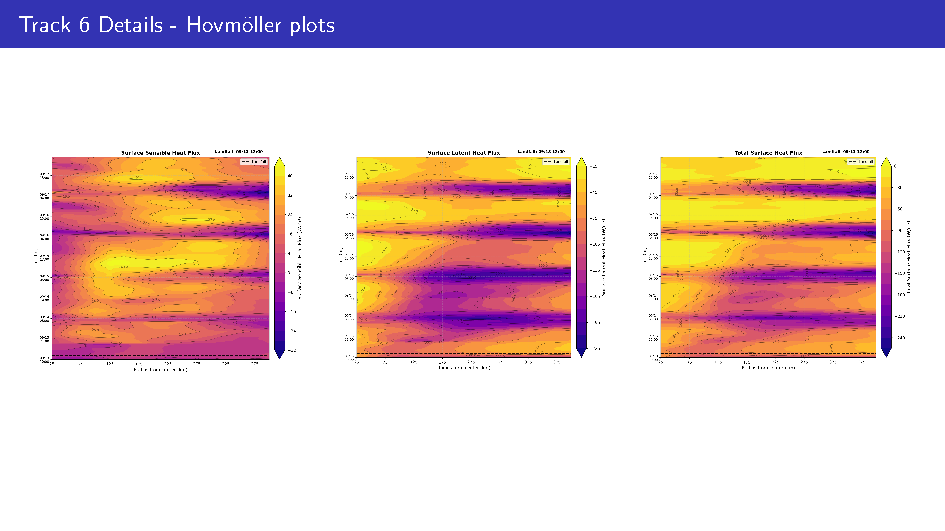
\includepdf[
    pages=-,
    scale=1,
    frame=true,
    % pagecommand={},
    pagecommand={\stepcounter{framenumber}},
    offset=0mm 0mm,       % Adjust position
    % templatesize={\textwidth}{\textheight} % Match template size
]{slides/hov-6.pdf}

\subsubsection{Track 6 \texttt{MODIS}}
\begin{frame}{\texttt{MODIS} Track 6 Visualization (2000m Scale)}
    \begin{center}
        \begin{figure}
            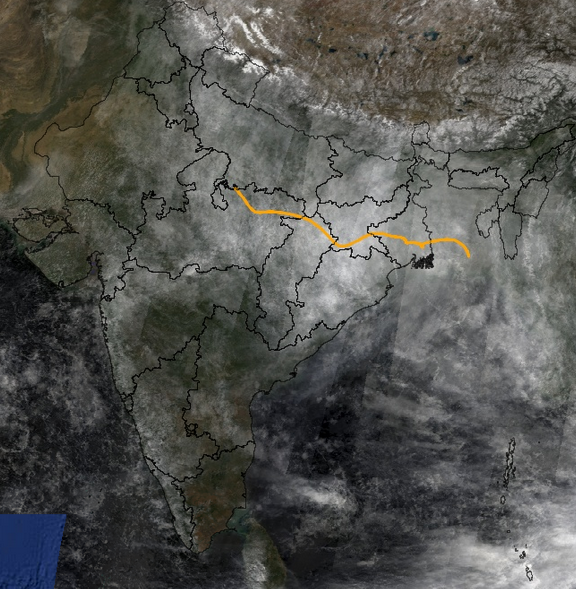
\includegraphics[width=0.45\linewidth]{images/MODIS-2024-Track_6.png}
        \end{figure}
        \label{fig:modistrack6}
    \end{center}

    % TODO:
    \vspace{0.2cm}
    {\tiny \textbf{Figure~\ref{fig:modistrack6} :} \texttt{MODIS} satellite image (true color) of Track. The characteristic depression cloud structure is visible with high Cloud cluster to the around/near track (like track 2 but unlike track 1, 4, 5) because of very low translation speed of MD centre. Image source: GEE, NASA \texttt{MODIS} Level 1B.}
\end{frame}

% %%%%%%%%%%%%%%%%%%%%%%%%%%
%                Statistical Results
% % FIX: update vlaues
% \begin{frame}{Diurnal SHF Amplitude}
%     \begin{table}[H]
%         \small
%         \centering
%         \begin{tabular}{lcccccc}
%             \toprule
%             \textbf{Track} & \textbf{Ocean Amp} & \textbf{Land Amp} & \textbf{$\Delta$ Amp} & \textbf{Mean SHF$_{land}$} & \textbf{Durtn} \\
%                            & (W/m$^2$)          & (W/m$^2$)         & (W/m$^2$)             & (W/m$^2$)                  & (h)            \\
%             \midrule
%             1              & 11.1               & 58.1              & 47.0                  & -11.0                      & 78             \\
%             2              & --                 & 57.8              & --                    & 8.3                        & 105            \\
%             3              & --                 & 65.3              & --                    & 5.3                        & 154            \\
%             4              & 13.0               & 59.3              & 46.3                  & -6.9                       & 75             \\
%             5              & 16.5               & 63.7              & 47.2                  & 13.4                       & 165            \\
%             6              & --                 & 61.5              & --                    & 13.7                       & 117            \\
%             \bottomrule
%                            &                    &                   & Mean: 47.1            &                            &                \\
%             \bottomrule
%         \end{tabular}
%         \caption{Diurnal SHF Amplitude and Mean Land-Phase SHF}
%     \end{table}
%
%     \vspace{0.3cm}
%     \footnotesize
%     \textbf{Key Finding:}
%     \begin{itemize}
%         \item Amplitude change is \textit{consistent} across all tracks ($\approx 47$ W/m$^2$)
%         \item Mean SHF over land distinguishes long-lived: positive SHF (Tracks 2, 3, 5, 6 $\rightarrow$ 105-165h) vs. negative (Tracks 1, 4 $\rightarrow$ 75h)
%     \end{itemize}
% \end{frame}

%%%%%%%%%%%%%%%%%%%%%%%%%%%%%%
\section{Observations}
\begin{frame}[plain, noframenumbering]
    \begin{center}
        \Huge \textcolor{blue}{\textbf{Observations}} \\
    \end{center}
\end{frame}

\subsection{Diurnal Oscillations \& Phase Shift Mechanism}
% Wave / Oscillatory Patterns in Hovm\"oller Diagrams

 % Diurnal signal strength        & Weak: amplitude SHF $\sim$5–20 W/m$^2$, low coherence & Strong and coherent                           \\
 % Flux uniformity                & High (homogeneous sea surface)                        & Low (due to land cover, soil type, orography) \\
 % Typical SHF amplitude          & $< 10$–$20$ W/m$^2$                                   & $40$–$100$ W/m$^2$ (daytime peaks)            \\
 % Response time to solar forcing & Slow and damped : 3-8 h lag, amplitude heavily reduced & Fast : 1-4 h lag, amplitude close to max      \\
 % % TODO: further analysis required
 % % Thermal inertia                & High : weeks-scale storage in 20–100 m mixed layer     & Low : hours-scale in top 10–30 cm soil             \\
 %   Increase in SHF daytime amplitude + emergence of \texttt{$\sim$24 hour} periodicity in Hovm\"oller diagrams land-origin tracks and for tracks after landfall

\begin{frame}{Diurnal Oscillations \& Phase Shift Mechanism}
    Strong periodic signals appear prominently after land contact (For Land-Origin MDs at time of origin while for Ocean-Origin MDs at time of landfall).

    \vspace{0.2cm}
    \footnotesize
    \textbf{Heat fluxes showing clear wave/oscillatory patterns :}
    \begin{itemize}
        \item \textbf{Sensible Heat Flux (\texttt{SHF}) :} Daytime peaks driven by solar heating.
        \item \textbf{Latent Heat Flux (\texttt{LHF}) :} Often phase-shifted relative to \texttt{SHF}.
        \item \textbf{Soil Temperature (\texttt{STL1}) :} Clear diurnal cycle (\texttt{2}-\texttt{4 K} amplitude).
        \item \textbf{\texttt{2m} Temperature (\texttt{T2M}) :} Damped oscillation following \texttt{STL1}.
    \end{itemize}

    \vspace{0.2cm}
    \footnotesize
    These oscillations have a period of \texttt{$\sim$24 hours} and emerge specifically as the \texttt{MD} center moves over land.
    \begin{enumerate}
        \item Oscillatory (wave) patterns in \textbf{Azimuthal radially average Hovm\"oller diagrams} are \textbf{diurnal} and strongly amplified by land-surface interaction.
        \item \textbf{Ocean vs. Land :} Patterns are absent over the ocean due to high thermal inertia. Over land, the contrast between daytime heating and nighttime cooling drives the \texttt{24-hour} flux signal.
    \end{enumerate}

    % TODO: udpate citation
    \begin{block}{The \texttt{LHF} Phase Shift Mechanism}
        Over land, \texttt{LHF} (evaporation) timing is regulated by \textbf{Soil Moisture (\texttt{SWVL1})}. The maintained high evaporation rates outside peak heating hours act as a primary signature of the \textbf{Brown Ocean Effect}. \cite{nair2011influence} % \textbf{Vapor Pressure Deficit}
    \end{block}

    \vfill
    \noindent\makebox[\linewidth]{\rule{\paperwidth}{0.4pt}}
    \vspace{-0.2cm}
    \tiny
    \begin{itemize}
        \item \textbf{Nair et al. (2011) \cite{nair2011influence} :} Demonstrated that soil moisture-atmosphere coupling sustains inland intensity via \texttt{LHF} "pumping."
    \end{itemize}
\end{frame}

% \begin{frame}{Ocean Thermal Inertia vs. Rapid Land Response}
%     \framesubtitle{Why Only Land-Origin or Post-Landfall Tracks Show Strong Diurnal Waves Pattern?}
%     % \framesubtitle{Why oscillations emerge exclusively over land}
%
%     \footnotesize
%     \begin{center}
%         \begin{tabular}{p{2cm} | p{3.5cm} | p{3.5cm}}
%             \toprule
%             \textbf{Property} & \textbf{Ocean Phase} & \textbf{Land Phase} \\
%             \midrule
%             \textbf{SHF Amplitude} & Weak (\texttt{5-20 W/m$^2$}) & Strong (\texttt{40-100 W/m$^2$}) \\
%             \textbf{Surface Response} & Damped (High thermal inertia) & Rapid (Low thermal inertia) \\
%             \textbf{Flux Uniformity} & High (Homogeneous surface) & Low (Heterogeneous soil/terrain) \\
%             \textbf{Solar Lag} & \texttt{3-8 hours} (Slow) & \texttt{1-4 hours} (Immediate) \\
%             \textbf{Energy Source} & Deep mixed layer (\texttt{20-100 m}) & Top soil layer (\texttt{0-7 cm}) \\
%             \bottomrule
%         \end{tabular}
%     \end{center}
%
%     \begin{block}{Signature of Land interaction in Hovm\"oller Diagrams}
%         The emergence of \texttt{$\sim$24-hour} periodicity marks the transition from oceanic moisture-driven dynamics to land-based thermal-coupling \cite{nair2011influence}.
%         \begin{itemize}
%             \item \textbf{Daytime \texttt{SHF}:} High-intensity "pumping" fuels convective instability.
%             \item \textbf{Nighttime \texttt{LHF} Shift:} Sustains the core moisture when solar heating is absent, preventing system collapse \cite{andersen2014insights}.
%         \end{itemize}
%     \end{block}
%
%     \vfill
%     \noindent\makebox[\linewidth]{\rule{\paperwidth}{0.4pt}}
%     \vspace{-0.2cm}
%     \tiny
%     \begin{itemize}
%         \item \cite{kishtawal2013tropical} : Validated that Indian monsoon soils provide sufficient energy for storm maintenance post-landfall.
%         \item \cite{andersen2014insights} : Defined the thermodynamic requirement for BoE: saturated soil providing a "pseudo-ocean" moisture supply.
%     \end{itemize}
% \end{frame}

\begin{frame}{Implications : Land-Coupling \& MD Longevity}
    \framesubtitle{How diurnal oscillations translate to inland maintenance}

    \footnotesize
    \begin{block}{The Diurnal Recharge Cycle}
        Over land, the \texttt{MD} survives by alternating its energy source :
        \begin{enumerate}
            \footnotesize
            \item \textbf{Daytime (\texttt{SHF} peak) :} Warms the boundary layer, lowering surface pressure and maintaining low-level convergence.
                \footnotesize
                \begin{itemize}
                    \tiny
                    \item Daytime SHF $\rightarrow$ warms boundary layer $\rightarrow$ helps maintain low-level convergence
                \end{itemize}
            \footnotesize
            \item \textbf{Nighttime (\texttt{LHF} shift) :} Prevents the drying out of the storm core by using soil moisture reservoirs(Moist soil) (\texttt{SWVL1}).
                \begin{itemize}
                    \tiny
                    \item Nighttime LHF $\rightarrow$ land supplies moisture to atmosphere in order to sustain convection overnight
                \end{itemize}
        \end{enumerate}
    \end{block}

    \footnotesize
    \begin{block}{Soil Moisture Memory \& Persistence}
        Unlike the ocean, land has \textbf{Memory} (\texttt{ACF} at \texttt{24h} lag).
        \begin{enumerate}
            \item High \texttt{SWVL1} from previous day precipitation (\texttt{TP}) pre-conditions the surface for today's \texttt{LHF} release.
                \begin{itemize}
                    \tiny
                    \item Soil moisture memory $\rightarrow$ preconditions next day's cycle
                \end{itemize}
            \item This self-sustaining feedback (\textbf{Brown Ocean Effect}) is allows Monsoon Depressions to persist for weeks over the Indian subcontinent \cite{kishtawal2013tropical}.
        \end{enumerate}
    \end{block}

    \footnotesize
    While the ocean provides a \textit{constant} supply, the land provides a \textit{pulsing} but efficient supply MDs depending on \textbf{Soil texture} and \textbf{Elevation}.

    \footnotesize
    \textbf{Contrast with ocean phase :}
    \begin{itemize}
        \tiny
        \item Nearly constant heat supply (small or negligible diurnal cycle).
        \item Moisture from large ocean reservoir.
    \end{itemize}

    \vfill
    \noindent\makebox[\linewidth]{\rule{\paperwidth}{0.4pt}}
    \vspace{-0.2cm}
    \tiny
    \begin{itemize}
        \item \cite{kishtawal2013tropical} : Validated that Indian monsoon soils provide sufficient energy for storm maintenance post-landfall.
    \end{itemize}
\end{frame}

% \subsection{Soil Moisture Memory (\texttt{ACF} Results)}
% \begin{frame}{Soil Moisture Memory (\texttt{ACF} Results)}
%     \vspace{-0.5cm}
%     \footnotesize
%     \begin{center}
%         \begin{table}
%             \centering
%             \caption{\footnotesize Autocorrelation Function (\texttt{ACF}) analysis of (\texttt{SWVL1}) at a 24-hour lag. The Memory Index quantifies the persistence of land surface moisture, where higher positive values indicate potential for sustained land-atmosphere feedback (Brown Ocean Effect).}
%             \begin{tabular}{lccccc}
%                 \toprule
%                 \textbf{Track} & \textbf{Memory Index (\texttt{ACF-24h})} & \textbf{Mean \texttt{SWVL1}} & \textbf{Category}    & \textbf{Duration} & \textbf{Inference}       \\
%                 \midrule
%                 1              & \texttt{-0.092}              & \texttt{0.140}               & Negative             & \texttt{75h}               & Oscillatory, no memory   \\
%                 2              & \texttt{-0.061}              & \texttt{0.399}               & Negative             & \texttt{105h}              & Draining despite high SM \\
%                 3              & \texttt{+0.321}              & \texttt{0.421}               & \textbf{Strong}      & \texttt{124h}              & Moderate persistence     \\
%                 4              & \texttt{-0.197}              & \texttt{0.178}               & Negative             & \texttt{65h}               & Weak retention           \\
%                 5              & \texttt{+0.525}              & \texttt{0.270}               & \textbf{Very Strong} & \texttt{163h}              & Excellent persistence    \\
%                 6              & \texttt{+0.034}              & \texttt{0.428}               & Weak                 & \texttt{112h}              & Minimal memory           \\
%                 \bottomrule
%             \end{tabular}
%         \end{table}
%     \end{center}
%
%     \vspace{0.1cm}
%     \begin{columns}[T]
%         \column{0.5\textwidth}
%         \begin{block}{\footnotesize \texttt{High Persistence} : Track 5}
%             \footnotesize
%             \begin{itemize}
%                 \item \texttt{ACF-24h} : \texttt{0.525} (Strongly Persistent)
%                 \item \textbf{Insight :} High moisture retention supported a \texttt{$\sim$6-day} inland journey. The soil acted as a stable fuel tank.
%             \end{itemize}
%         \end{block}
%
%         \column{0.5\textwidth}
%         \begin{block}{\footnotesize \texttt{Anti-persistent} : Track 4}
%             \footnotesize
%             \begin{itemize}
%                 \item \texttt{ACF-24h} : \texttt{-0.197} (Oscillatory)
%                 \item \textbf{Insight :} Rapid moisture fluctuations and high surface "noise" led to system decay within \texttt{$\sim$3 days}.
%             \end{itemize}
%         \end{block}
%     \end{columns}
%
%     \vspace{0.2cm}
%     \footnotesize
%     \textbf{Physical Interpretation of \texttt{Memory Index}:}
%     \begin{itemize}
%         \item \texttt{ACF-24h > 0.3} : Sustained \texttt{LHF} release via the \textbf{Brown Ocean Effect}. Soil stores moisture between diurnal peaks.
%         \item \texttt{ACF-24h < 0} : Fast "Dry-down" or rapid evaporation. Surface cannot maintain a constant thermodynamic supply to the core.
%     \end{itemize}
%
%     \vspace{0.2cm}
%     \footnotesize
%     \textbf{Classification Thresholds:}
%     \begin{itemize}
%         \item \textbf{Very Strong Memory}: \texttt{ACF > 0.3} (Track 5) $\rightarrow$ Highest multi-day feedback.
%         \item \textbf{Strong Memory}: \texttt{0.1 < ACF < 0.3} (Track 3) $\rightarrow$ Moderate persistence.
%         \item \textbf{Weak/Negative Memory}: \texttt{ACF < 0.1} (Tracks 1, 2, 4, 6) $\rightarrow$ Rapid dry-down or noise.
%     \end{itemize}
% \end{frame}
%
% \subsection{Terrain Strength Index (\texttt{TSI})}
% % Why Might 2024 Have Higher TSI?
% % Wetter Soil Effect:
% %     - 2024 wet soil (0.316) vs 2023 dry soil (0.169)
% %     - Wetter terrain -> different heating -> different orographic effects
% %     Different Track Locations:
% %     - May have occurred over more mountainous regions
% %     - Different routes -> different terrain sensitivity
% %     Different Track Orientations:
% %     - Relative to mountain ranges
% %     - Affects how much terrain influences depression
% %     Atmospheric Conditions:
% %     - Different wind shear profiles
% %     - Different CAPE distributions
% %     - Affect how terrain modulates flow
% % Interpretation:
% % - Topography effects are NOT constant across years
% % - They depend on environmental conditions
% % - Makes operational prediction more complex
% % - Need to include both terrain AND environmental state
% \begin{frame}{Terrain Strength Index (\texttt{TSI})}
%     \vspace{-0.5cm}
%     \footnotesize
%     \begin{center}
%         \begin{table}
%             \centering
%             \caption{}
%             \begin{tabular}{lccccc}
%                 \toprule
%                 \midrule
%                 \bottomrule
%             \end{tabular}
%         \end{table}
%     \end{center}
%
%     \vspace{0.1cm}
%     \begin{columns}[T]
%         \column{0.5\textwidth}
%         \begin{block}{}
%             \footnotesize
%             \begin{itemize}
%                 \item
%                 \item
%             \end{itemize}
%         \end{block}
%
%         \column{0.5\textwidth}
%         \begin{block}{}
%             \footnotesize
%             \begin{itemize}
%                 \item
%             \end{itemize}
%         \end{block}
%     \end{columns}
%
%     \vspace{0.2cm}
%     \footnotesize
%     \textbf{Physical Interpretation of \texttt{Memory Index}:}
%     \begin{itemize}
%         \item
%         \item
%     \end{itemize}
%
%     \vspace{0.2cm}
%     \footnotesize
%     \textbf{Classification Thresholds:}
%     \begin{itemize}
%         \item
%     \end{itemize}
% \end{frame}
%
% \subsection{Heat Flux Transitions : Ocean-to-Land Cases}
% \begin{frame}{Heat Flux Transitions : Ocean-to-Land Cases}
%     \begin{table}[H]
%         \footnotesize
%         \centering
%         \caption{Mean Heat Fluxes (\texttt{W/m$^2$}) for 24h windows around landfall. Positive $\Delta$ indicates energy loss at landfall.}
%         \begin{tabular}{lccccccc}
%             \toprule
%                            & \multicolumn{3}{c}{\textbf{Before Landfall}} & \multicolumn{3}{c}{\textbf{After Landfall}} &                \\
%             \cmidrule(lr){2-4} \cmidrule(lr){5-7}
%             \textbf{Track} & \texttt{LHF} & \texttt{SHF} & \texttt{THF} & \texttt{LHF} & \texttt{SHF} & \texttt{THF} & $\Delta$ \textbf{Total} \\
%             \midrule
%             1              & \texttt{-133} & \texttt{-10.2} & \texttt{-143} & \texttt{-97} & \texttt{-4.4} & \texttt{-101} & \texttt{+42} \\
%             4              & \texttt{-155} & \texttt{-15.0} & \texttt{-170} & \texttt{-97} & \texttt{-8.6} & \texttt{-105} & \texttt{+65} \\
%             5              & \texttt{-135} & \texttt{-12.2} & \texttt{-147} & \texttt{-81} & \texttt{+4.3} & \texttt{-77}  & \texttt{+70} \\
%             \bottomrule
%         \end{tabular}
%     \end{table}
%
%     \vspace{0.2cm}
%     \footnotesize
%     \textbf{Interpretation :}
%     \begin{itemize}
%         \item \textbf{Energy Retention :} \texttt{LHF} remains high post-landfall (\texttt{81--97 W/m$^2$}), retaining $>\texttt{60\%}$ of oceanic moisture supply.
%         \item \textbf{Brown Ocean Signature :} Sustained \texttt{LHF} over land indicates that saturated soil is replacing the ocean as the primary moisture source.
%         \item \textbf{\texttt{SHF} Reversal :} In Track 5, \texttt{SHF} turns positive (\texttt{+4.3 W/m$^2$}), showing the land surface heating the atmosphere, typical of a daytime land-coupled MD, suggesting marks the transition to land-based thermal forcing.
%     \end{itemize}
% \end{frame}
%
% \subsection{Lag Correlation Analysis (\texttt{TP}-\texttt{SWVL1})}
% \begin{frame}{Lag Correlation Analysis : \texttt{TP}-\texttt{SWVL1}}
%     \footnotesize
%     \textbf{Interpretation : Lag Logic for \texttt{r(Lag)}}
%     \begin{itemize}
%         \item \textbf{Positive Lags (\texttt{+})} : \textit{Soil Moisture Leads.} \texttt{SWVL1} state predicts future \texttt{TP} (Land $\rightarrow$ Atmosphere feedback).
%         \item \textbf{Negative Lags (\texttt{-})} : \textit{Precipitation Leads.} \texttt{TP} infiltration recharges soil (Atmosphere $\rightarrow$ Land / Infiltration).
%         \item \textbf{Zero Lag (\texttt{0})} : Simultaneous coupling (High efficiency, Immediate recharge/feedback).
%     \end{itemize}
%
%     \vspace{0.2cm}
%     \footnotesize
%     \textbf{Observed Peak Correlations (\texttt{Max |r|}) by Track :}
%     \begin{center}
%         \footnotesize
%         \begin{tabular}{c c c l p{5cm}}
%             \toprule
%             \textbf{Track} & \textbf{Peak Lag} & \textbf{Max |r|} & \textbf{Sign} & \textbf{Physical Interpretation} \\
%             \midrule
%             1 & \texttt{+24 h} & \texttt{0.26} & Negative & Diurnal antecedent moisture feedback cycle. \\
%             2 & \texttt{+17 h} & \texttt{0.57} & Positive & Strongest land-driven recycling. \\
%             3 & \texttt{$\sim$0 h} & \texttt{0.84} & Positive & Highest coupling efficiency (\texttt{15.35}). \\
%             4 & \texttt{-23 h} & \texttt{0.28} & Negative & \texttt{TP} leads; Significant infiltration delay. \\
%             5 & \texttt{$\sim$0 h} & \texttt{0.44} & Positive & Stable, simultaneous feedback loop. \\
%             6 & \texttt{+4 h} & \texttt{0.56} & Negative & Convective triggering; moisture leads rain. \\
%             \bottomrule
%         \end{tabular}
%     \end{center}
%
%     \footnotesize
%     \begin{block}{Insights :}
%         \begin{itemize}
%             \item \textbf{Track 3 :} Validated as the strongest coupling strength (\texttt{r=0.8418}) and highest Coupling Efficiency.
%             \item \textbf{Track 6 Anomaly :} Moderate negative correlation (\texttt{r=-0.5620}) despite being a long-lived MD.
%             \item \textbf{Soil Moisture Leads (Tracks 1, 2, 6) :} Indicates land-driven feedback where antecedent soil moisture may trigger later precipitation events.
%             \item \textbf{Lag Anomaly (Track 4) :} Very long infiltration delay, the \texttt{-23h} lag indicates the storm is moisture-limited; rainfall occurs but soil response is too slow to provide immediate feedback. (maybe due dense soils or deep sensor placements)
%             %\textbf{Anomalous Lag (Track 4):} The \texttt{-23h} lag suggests "Precipitation dominance"—the storm is dumping water, but the surface isn't providing a prompt feedback.
%             \item \textbf{Zero Lag (Tracks 3, 5) :} Represents tightly coupled systems with near-instantaneous surface wetting, essential for maintaining MD core structure.
%             % \item \textbf{Coupling Efficiency:} Tracks \texttt{3} and \texttt{5} demonstrate "Zero-Lag" coupling, maintaining core thermodynamics via near-instantaneous surface wetting.
%         \end{itemize}
%     \end{block}
% \end{frame}
%
% \subsection{Diurnal \texttt{SHF} Amplitude} % ($A_{\text{\texttt{SHF}}}$) }
% \begin{frame}{Diurnal Sensible Heat Flux : Land Amplifies Surface Heating}
%     \begin{columns}[T]
%         \column{0.30\textwidth}
%             \footnotesize
%             \textbf{Amplitude :}
%             \begin{itemize}
%                 \item \textbf{Land phase :} \texttt{56.26 W/m$^2$}
%                 \item \textbf{Ocean phase :} \texttt{13.54 W/m$^2$}
%             \end{itemize}
%
%         \column{0.36\textwidth}
%             \footnotesize
%             \textbf{Land-phase Amplitudes :}
%             \begin{itemize}
%                 \item Track 3 : \texttt{62.3 W/m$^2$}
%                 \item Track 4 : \texttt{59.6 W/m$^2$}
%                 \item Track 5 : \texttt{63.7 W/m$^2$}
%             \end{itemize}
%
%         \column{0.31\textwidth}
%             \footnotesize
%             \textbf{Transition Surge :}
%             \begin{itemize}
%                 \item Track 1 : \texttt{+44.1 W/m$^2$}
%                 \item Track 4 : \texttt{+46.6 W/m$^2$}
%                 \item Track 5 : \texttt{+47.2 W/m$^2$}
%             \end{itemize}
%     \end{columns}
%
%     \vspace{0.4cm}
%     \footnotesize
%     \textbf{Interactions :}
%     \begin{itemize}
%         \item \textbf{Thermal Inertia :} Oceans damp diurnal cycles (\texttt{13.54 W/m$^2$}) while land's low thermal inertia drives massive daytime \texttt{SHF} spikes.
%         \item \textbf{Boundary Layer :} High \texttt{SHF} amplitudes post-landfall (\texttt{> 60 W/m$^2$}) indicate land surfaces actively forcing convection.
%     \end{itemize}
% \end{frame}
%
% \subsection{Feedback Strength Index (\texttt{FSI})}
% % values from coupling_metrics_FSI.csv and coupling_metrics_efficiency.csv
% \begin{frame}{Feedback Strength Index (\texttt{FSI}) : \texttt{TP}-\texttt{SWVL1} Coupling Efficiency}
%     \begin{center}
%         \begin{columns}[T]
%             \column{0.67\textwidth}
%             \footnotesize
%             \begin{table}[h]
%                 \caption{FSI, Coupling Efficiency (CE), and Track Characteristics.}
%                 \begin{tabular}{lccccc}
%                     \toprule
%                     \textbf{Track} & \textbf{FSI} & \textbf{CE} & \textbf{Corr. ($|r|$)} & \textbf{Capacity} & \textbf{Dur. (h)} \\
%                     \midrule
%                     1              & \texttt{0.060} & \texttt{3.41}  & \texttt{0.26} & \texttt{0.23} & \texttt{75}  \\
%                     2              & \texttt{0.406} & \texttt{10.37} & \texttt{0.57} & \texttt{0.72} & \texttt{105} \\
%                     3              & \texttt{0.637} & \texttt{15.35} & \texttt{0.84} & \texttt{0.76} & \texttt{124} \\
%                     4              & \texttt{0.084} & \texttt{4.66}  & \texttt{0.28} & \texttt{0.30} & \texttt{65}  \\
%                     5              & \texttt{0.208} & \texttt{7.61}  & \texttt{0.44} & \texttt{0.47} & \texttt{163} \\
%                     6              & \texttt{0.432} & \texttt{10.74} & \texttt{0.56} & \texttt{0.77} & \texttt{112} \\
%                     \midrule
%                     \textbf{Mean}  & \texttt{0.305} & \texttt{8.69}  & \multicolumn{3}{l}{$\sigma = \pm \texttt{0.23}$ (FSI)} \\
%                     \bottomrule
%                 \end{tabular}
%             \end{table}
%
%             \column{0.33\textwidth}
%             \vspace{0.5cm}
%             \footnotesize
%             \begin{itemize}
%                 \item \textbf{High FSI :} Efficient precipitation-soil moisture feedback loop.
%                 \item \textbf{Low FSI :} Inefficient or decoupled land-atmosphere response or negative feedback.
%             \end{itemize}
%             \vspace{0.4cm}
%             Higher FSI indicates more efficient moisture-driven energy exchange between land and MD.
%         \end{columns}
%
%         \vspace{0.3cm}
%         \begin{block}{Interpretation: \footnotesize The Efficiency Threshold}
%             \footnotesize
%             \begin{itemize}
%                \item \textbf{Longevity Threshold:} Tracks with \texttt{FSI > 0.40} (2, 3, 6) survive $\geq \texttt{105h}$. Tracks with \texttt{FSI < 0.10} (1, 4) dissipate by $\approx \texttt{70h}$.
%                \item \textbf{Positive Feedback (2, 3, 5):} Active soil moisture recharge cycles back to rainfall (\texttt{SM} $\rightarrow$ \texttt{Rainfall}).
%                \item \textbf{Anomalous Persistence (Track 5):} Achieves \texttt{163h} duration despite "Moderate" FSI (\texttt{0.208}), suggesting atmospheric factors (e.g., strong mid-level vorticity) compensate for lower coupling.
%
%                \item \textbf{Negative Correlation tracks (1, 4, 6) :} Shows complex lag effects or instantaneous soil moisture drying/runoff during peak rain events. Rainfall $\rightarrow$ Soil moisture infiltration. \cite{clapp1978empirical}
%             \end{itemize}
%         \end{block}
%     \end{center}
% \end{frame}
%
% \subsection{Coupling Efficiency (\texttt{CE})}
% \begin{frame}{Defining Land-Atmosphere Coupling Efficiency}
%     \begin{block}{What is 'Coupling'? (Soil-Moisture Feedback)}
%         \footnotesize
%         \textit{Physical Mechanism: The "Brown Ocean"-like} \\
%         In this study, \textbf{Coupling} refers to the thermodynamic link between the \textbf{land surface} and the \textbf{centre/core/vortex} of MD structure :
%         \begin{itemize}
%             \item \textbf{Flux Transfer :} Moist soil provides Latent Heat Flux (\texttt{LHF}), replacing the ocean's moisture supply.
%             \item \textbf{Energy Pulse :} Daytime Sensible Heat Flux (\texttt{SHF}) creates the instability required to "lift" moisture into the core.
%             \item \textbf{Coupling Efficiency (\texttt{CE}) :} A measure of how effectively a "pulse" of soil moisture is converted into sustained atmospheric heating to prevent the MD from dissipating.
%         \end{itemize}
%     \end{block}
%
%     \vspace{0.2cm}
%     \textbf{Mathematical Formulation :} \\
%     Feedback Strength Index (\texttt{FSI}) :
%     \begin{equation}
%         \text{\texttt{FSI}} = |r| \times \text{Capacity} \times \text{Significance}
%     \end{equation}
%
%     and Coupling Efficiency (\texttt{CE}) \ref{eq:couplingeff} :
%     \begin{equation}
%         \text{\texttt{CE}} = \text{\texttt{FSI}} \times \text{\texttt{A}}_{SHF} \times \text{Duration Factor}
%     \end{equation}
%
%     \vfill
%     {\let\thefootnote\relax\footnotetext{\tiny *Note: Significance is a binary (0 or 1) based on p-value \texttt{< 0.05}.}}
% \end{frame}
%
% % values from coupling_metrics_efficiency.csv
% \begin{frame}{Quantitative Coupling Analysis}
%     \vspace{-0.3cm}
%     \begin{table}[H]
%         \footnotesize
%         \centering
%         \caption{Thermodynamic coupling metrics across all MD tracks.}
%         \begin{tabular}{lcccccc}
%             \toprule
%             \textbf{Track} & \textbf{FSI} & \textbf{SHF Amp.} & \textbf{Memory (\texttt{ACF})} & \textbf{CE} & \textbf{Duration} & \textbf{Status} \\
%             \midrule
%             1 & \texttt{0.060} & \texttt{55.1} & \texttt{-0.092} & \texttt{2.11}  & \texttt{75h}  & Short/Weak \\
%             2 & \texttt{0.406} & \texttt{57.8} & \texttt{-0.061} & \texttt{10.74} & \texttt{105h} & \textbf{Efficient} \\
%             3 & \texttt{0.637} & \texttt{62.3} & \texttt{0.321}  & \texttt{15.35} & \texttt{124h} & \textbf{Peak Loop} \\
%             4 & \texttt{0.084} & \texttt{59.6} & \texttt{-0.197} & \texttt{3.68}  & \texttt{65h}  & Short/Weak \\
%             5 & \texttt{0.208} & \texttt{63.7} & \texttt{0.525}  & \underline{\texttt{3.90}}  & \texttt{163h} & \textit{Memory-Sustained} \\
%             6 & \texttt{0.432} & \texttt{39.1} & \texttt{0.034}  & \texttt{7.23}  & \texttt{112h} & \textbf{Efficient} \\
%             \midrule
%             \textbf{Mean} & \texttt{0.305} & \texttt{56.3} & \texttt{0.088} & \texttt{7.17} & \texttt{107h} & \\
%             \bottomrule
%         \end{tabular}
%     \end{table}
%
%     \footnotesize
%     \begin{block}{Patterns observed}
%         \begin{itemize}
%             \item \textbf{Land-origin tracks (2, 3, 6)} generally have significantly higher coupling efficiency ($>7.0$). Soil moisture memory (\texttt{ACF}) and high capacity in the Indo-Gangetic plains (with clay soil) provide a stable conditions for these tracks to sustain longer.
%             \item \textbf{Ocean-origin short-lived tracks (1, 4)} have the lowest efficiency (\textbf{\textit{due to sandy soils (low capacity)?}}).
%             \item Ocean-origin long-lived track (5) survives \texttt{163h} despite low \texttt{CE (3.90)}. High \texttt{ACF (0.525)} acts as a "buffer" for energy supply. Also other reason could be large-scale atmospheric forcing (vorticity/moisture advection) rather than local land-surface coupling.
%         \end{itemize}
%     \end{block}
% \end{frame}
%
% % values from coupling_metrics_efficiency.csv and coupling_metrics_FSI.csv
% \subsection{Track Classification}
% \begin{frame}{Track Classification by Coupling Strategy}
%     \footnotesize
%     \begin{center}
%         \begin{columns}[T]
%             \column{0.30\textwidth}
%             \textbf{I. Strongly Coupled} \textit{(Tracks 2, 3, 6)}
%             \begin{itemize}
%                 \item \textbf{FSI:} \texttt{0.41 -- 0.64}
%                 \item \textbf{CE :} \texttt{7.23 - 15.35}
%                 \item \textbf{Duration :} \texttt{105 -- 124 h}
%                 \item High baseline SM 
%                 \item \textbf{High SM (soil was already moist) + positive feedback}
%             \end{itemize}
%
%             \column{0.37\textwidth}
%             \textbf{II. Memory Sustained} \textit{(Track 5)}
%             \begin{itemize}
%                 \item \textbf{FSI :} \texttt{0.21}
%                 \item \textbf{CE :} \texttt{3.90}
%                 \item \textbf{Duration :} \texttt{163 h}
%                 \item \textbf{Memory :} \texttt{ACF-24h = 0.525}
%                 \item High persistence (\texttt{ACF=0.52}). Persists through atmospheric forcing + soil "buffer."
%                 \item \textit{Anomaly}. Longest track via soil buffer.
%             \end{itemize}
%
%             \column{0.35\textwidth}
%             \textbf{III. Weakly Coupled} \textit{(Tracks 1, 4)}
%             \begin{itemize}
%                 \item \textbf{FSI :} \texttt{0.06 -- 0.08}
%                 \item \textbf{CE :} \texttt{2.11 - 3.68}
%                 \item \textbf{Duration :} \texttt{65 -- 75 h}
%                 \item Rapid decay following landfall due to negative SM memory.
%             \end{itemize}
%         \end{columns}
%     \end{center}
%
%     \begin{block}{\footnotesize Longevity is driven by two distinct modes :}
%         \begin{enumerate}
%             \footnotesize
%             \item \textbf{Efficiency Mode :} High \texttt{CE} fuels the low pressure system (Tracks 2, 3, 6).
%             \item \textbf{Persistence Mode :} High \texttt{Memory} buffers the low pressure system (Track 5).
%         \end{enumerate}
%         \footnotesize
%         Short-lived Ocean-origin (Coastal) tracks lack both and dissipate shortly.
%     \end{block}
%
%     \footnotesize
%     \begin{block}{Key Patterns observed}
%         \begin{itemize}
%             \item \textbf{Direct Coupling :} For 5 out of 6 tracks (with exception of track 5), longevity is a linear function of coupling efficiency (higher \texttt{CE} = more hours over land).
%             \item \textbf{The Buffer Effect :} Track 5 proves that \textbf{Soil Moisture Memory} acts as a secondary survival mechanism. Even with moderate dynamic coupling, high autocorrelation (\texttt{0.525}) prevents rapid collapse.
%             % \item \textbf{Origin Impact :} Tracks originating/spending time over land establish more efficient feedback loops than those making sudden coastal transitions.
%         \end{itemize}
%     \end{block}
% \end{frame}
%
% \subsection{Heat Flux Analysis - Energy Budget}
% % values from heat_flux_analysis_summary.csv and heat_flux_transitions.csv
% % FIX: provide individual tracks values instead of Mean fluxes
% \begin{frame}[label=budget]{Heat Flux Analysis : The Surface Energy Budget}
%     \begin{columns}[T]
%         \column{0.5\textwidth}
%         \footnotesize
%         \begin{block}{Surface Flux Statistics (Land Phase)}
%             \centering
%             \begin{tabular}{lc}
%                 \toprule
%                 \textbf{Parameter} & \textbf{Mean Value}\footnotemark[6] \\
%                 \midrule
%                 Total Heat Flux & \texttt{-80.8 $\pm$ 40.1 W/m$^2$} \\
%                 Latent Flux (\texttt{LHF}) & \texttt{-82.9 W/m$^2$} \\
%                 Sensible Flux (\texttt{SHF}) & \texttt{+2.1 W/m$^2$} \\
%                 \bottomrule
%             \end{tabular}
%         \end{block}
%
%         \column{0.5\textwidth}
%         \footnotesize
%         \begin{block}{Heat Flux Landfall Transition (Ocean $\rightarrow$ Land)}
%             \centering
%             \begin{tabular}{lc}
%                 \toprule
%                 \textbf{Phase} & \textbf{Total Heat Flux} \\
%                 \midrule
%                 Before Landfall & \texttt{-142.1 W/m$^2$} \\
%                 After Landfall & \texttt{-90.9 W/m$^2$} \\
%                 \textbf{Change ($\Delta$)} & \textbf{\texttt{+51.2 W/m$^2$}} \\
%                 \bottomrule
%             \end{tabular}
%         \end{block}
%     \end{columns}
%
%     \vspace{0.4cm}
%     \footnotesize
%     \textbf{Interpretation :}
%         \begin{itemize}
%             \item \textbf{Latent Heat Dominance :} \texttt{LHF} is the primary energy driver (\texttt{$\approx$ 83 W/m$^2$}) over land. By converting soil moisture into atmosphere moisture (via evaporation) sustain  the MD's core.
%             \item \textbf{The "Moisture Cut-off" :} Total heat flux becomes significantly less negative upon landfall (\texttt{+51.2 W/m$^2$} change).  The \texttt{+51.2 W/m$^2$} change indicates the system is receiving significantly less moisture from land than it did from the ocean. This represents the reduction in moisture availability (moisture cut-off) while sensible heating from the land surface increases. Longevity depends on how slowly this "decay" happens.
%             \item \textbf{Thermodynamic Maintenance :} The negative total flux implies the surface is cooling. To maintain the vortex, the MD must rely on the internal release of Latent Heat (condensation) within the core to overcome surface losses.
%         \end{itemize}
%
%     \footnotetext[6]{\tiny Averaged across all tracks during the land-only phase.}
% \end{frame}
%
% \subsection{Diurnal \texttt{SHF} Amplitude} % ($A_{\text{\texttt{SHF}}}$) }
% % values from coupling_metrics_diurnal_amplitude.csv
% \begin{frame}{Diurnal Sensible Heat Flux (\texttt{SHF}) Amplitude}
%     \vspace{-0.5cm}
%     \begin{columns}[T]
%         \column{0.6\textwidth}
%         \footnotesize
%         \begin{block}{Land-Ocean Phase Comparison}
%             \centering
%             \begin{tabular}{lcc}
%                 \toprule
%             \textbf{Phase} & \textbf{Mean \texttt{SHF} Amplitude} & \textbf{\(\Delta\)\texttt{SHF}} \\
%                                &  \texttt{$\left(\frac{\Sigma \texttt{SHF}_{\texttt{24}}}{\texttt{24 h}}\right)$} &  \texttt{$\left(\texttt{SHF}_{\text{max}} - \texttt{SHF}_{\text{min}}\right)$} \\
%                 \midrule
%                 Ocean phase & \texttt{+13.54 W/m$^2$} & \texttt{-11.66 W/m$^2$} \\
%                 Land phase  & \texttt{+56.26 W/m$^2$} & \texttt{+4.45 W/m$^2$} \\
%                 \midrule
%                 \textbf{Difference} & \textbf{\texttt{+42.72 W/m$^2$}} & \textbf{\texttt{+16.11 W/m$^2$}} \\
%                 \bottomrule
%             \end{tabular}
%         \end{block}
%
%         \column{0.4\textwidth}
%         \vspace{0.8cm}
%         \begin{center}
%             \footnotesize
%             \textit{Over land, the diurnal cycle is} \\
%             \large \textbf{$\approx$4 times Stronger} \\
%             \footnotesize \textit{than over the ocean,\\ driven by the land surface's lower heat capacity.}
%         \end{center}
%     \end{columns}
%
%     \vspace{0.6cm}
%     \footnotesize
%     \textbf{Physical Implications for MD Longevity :}
%     \begin{itemize}
%         \item \textbf{Thermal Forcing :} Upon landfall, the surface switches from a heat sink to a \textbf{heat source} (\texttt{\(\Delta\)SHF} turns positive).
%         \item \textbf{The "Convective Pump" :} The \texttt{+56.26 W/m$^2$} daily amplitude acts as a periodic trigger, destabilizing the boundary layer and lifting soil-derived moisture into the MD core. This enhanced diurnal heating compensates for the loss of ocean moisture, particularly in high-capacity soil regions (Land origin Tracks 2, 3, 6).
%         \item \textbf{System Maintenance :} This massive increase in diurnal forcing is what allows "Strongly Coupled" tracks (2, 3, 6) to maintain vortex intensity despite the loss of consistent oceanic evaporation.
%         \item \textbf{Directional Shift :} \texttt{SHF} becomes positive (upward$\uparrow$) over land, indicating the land surface is directly heating the MD's environment during the day.
%         \item \textbf{Thermodynamic Coupling :} The high diurnal amplitude over land (\texttt{+56.26 W/m$^2$}) fuels the Coupling Efficiency (\texttt{CE}) metric, providing the energy pulses needed to sustain convection.
%     \end{itemize}
% \end{frame}
%

\subsection{Elevation map}
\begin{frame}[label=elevationmap]{Elevation Map}
    \vspace{-0.5cm}
    \begin{columns}[T]
        \column{0.49\textwidth}
        \vspace{-0.02cm}
        \begin{figure}
           \includegraphics[width=1.1\linewidth]{../version21-with-no-ocean-masking/output_2024/MD_track_2024.png}
        \end{figure}

        \column{0.49\textwidth}
        \vspace{-0.02cm}
        \begin{figure}
            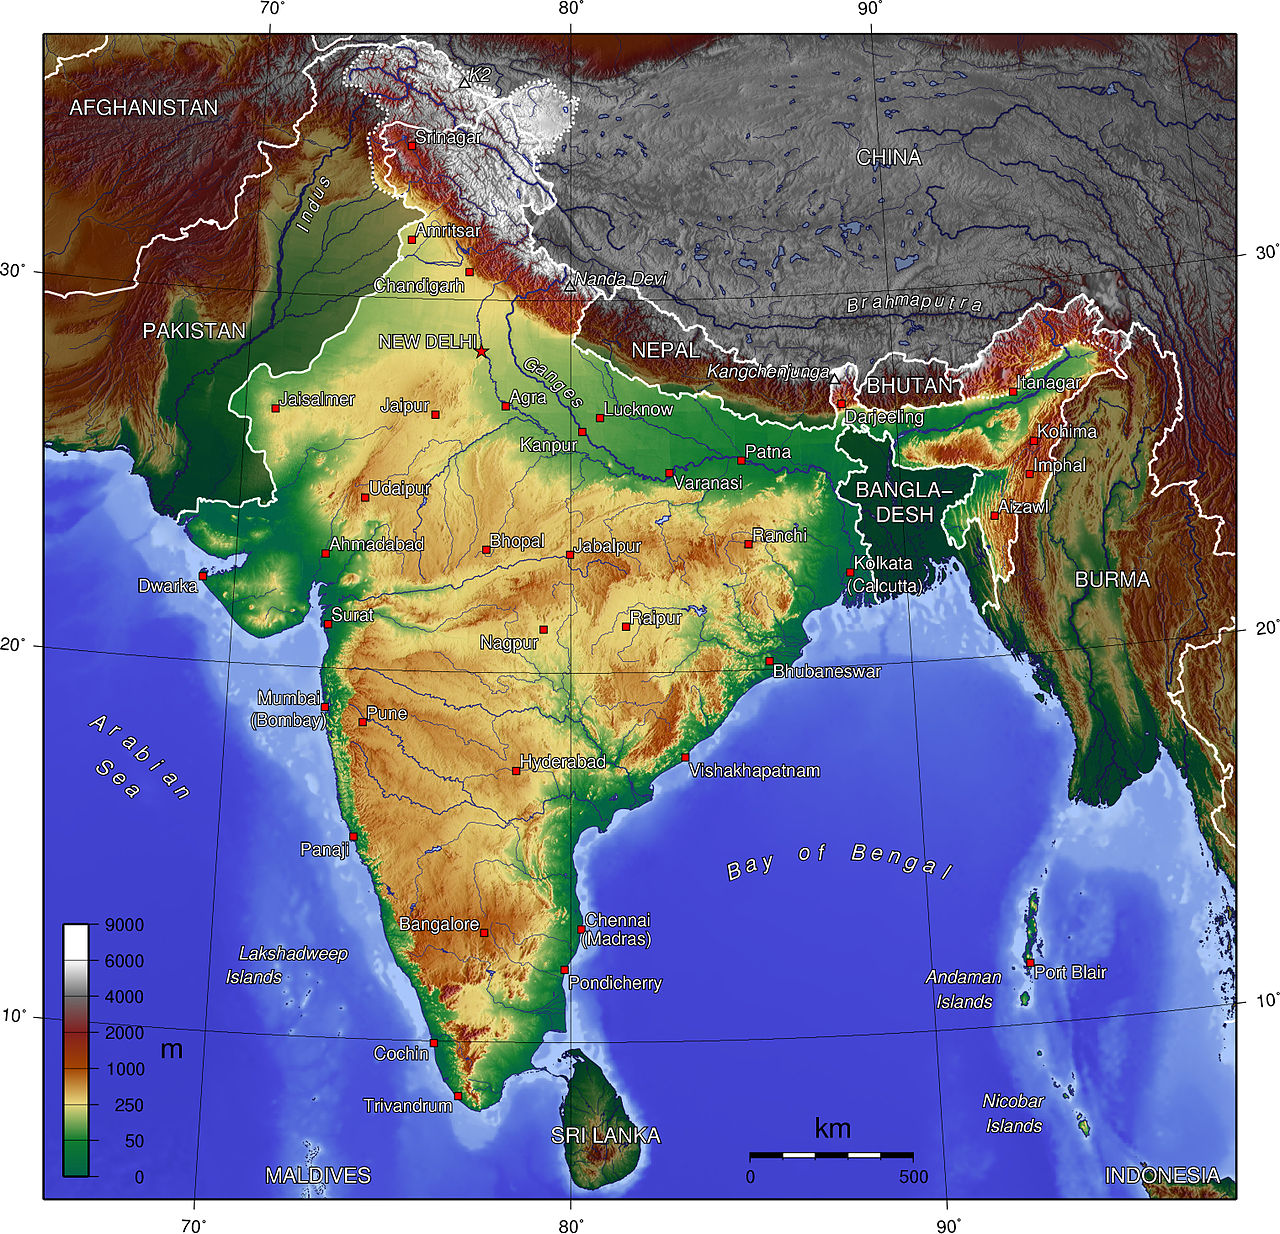
\includegraphics[width=\linewidth]{images/Elevation-map-of-India.jpg}
        \end{figure}
        \label{fig:elevationmapofindia}
        \tiny \textbf{Figure~\ref{fig:elevationmapofindia} :} Elevation map of India\footnotemark[7].
    \end{columns}
    \footnotetext[7]{Source : \href{https://commons.wikimedia.org}{\url{https://commons.wikimedia.org/wiki/File:India\_topo\_big.jpg}}}
\end{frame}

% \subsection{Soil Moisture Memory (\texttt{ACF-24h})}
% % values from all_tracks_soil_memory.csv
% \begin{frame}{Soil Moisture Memory (\texttt{ACF-24h}) : The Persistence Factor}
%     \begin{table}[H]
%         \footnotesize
%         \centering
%         \caption{Soil Moisture Autocorrelation at 24-hour Lag (\texttt{ACF-24h})}
%         \begin{tabular}{lcccccc}
%             \toprule
%             \textbf{Track} & \textbf{ACF-24h} & \textbf{Category} & \textbf{Mean SWVL1} & \textbf{Std SWVL1} & \textbf{Duration} & \textbf{Interpretation} \\
%             \midrule
%             1 & \texttt{-0.092} & Weak Neg. & \texttt{0.140} & \texttt{0.164} & \texttt{75h} & Rapid Depletion \\
%             2 & \texttt{-0.061} & Weak Neg. & \texttt{0.399} & \texttt{0.067} & \texttt{105h} & High Baseline/Low Carryover \\
%             3 & \texttt{0.321}  & \textbf{Moderate} & \texttt{0.421} & \texttt{0.047} & \texttt{124h} & \textbf{Persistent Pulse} \\
%             4 & \texttt{-0.197} & Weak Neg. & \texttt{0.178} & \texttt{0.186} & \texttt{65h} & Low Retention \\
%             \textbf{5} & \textbf{0.525} & \textbf{Strong} & \texttt{0.270} & \texttt{0.207} & \textbf{163h} & \textbf{Strategic Persistence} \\
%             6 & \texttt{0.034}  & Neutral   & \texttt{0.428} & \texttt{0.054} & \texttt{112h} & Saturated/Low Variance \\
%             \bottomrule
%         \end{tabular}
%     \end{table}
%
%     \footnotesize
%     \begin{block}{Key Findings :}
%         \begin{itemize}
%             \item \textbf{The Survival Buffer :} Track 5 survives \texttt{163h} (the longest) despite moderate \texttt{CE}. Its \texttt{ACF} of \texttt{0.525} acts as an energy "battery" that sustains the vortex during dynamic forcing (like elevated terrain, lower soil moisture(\texttt{SWVL1}). Thus Memory Index \texttt{ACF} compensates for its lower immediate coupling efficiency by providing a steady energy source.
%             \item \textbf{Memory Threshold :} Long-lived tracks (2, 3, 5, 6) all maintain non-negative or positive memory, whereas short-lived tracks (1, 4) show negative autocorrelation (\texttt{ACF < 0}), indicating "oscillatory" behavior $\Rightarrow$ moisture is lost faster than it can be recycled,  rapid moisture depletion.
%             \item \textbf{Inland Stability :} Track 3 shows the best combination of high baseline moisture (\texttt{0.42 m$^3$/m$^3$}) and moderate memory (\texttt{0.321}), fueling the highest coupling efficiency observed among all tracks.
%         \end{itemize}
%     \end{block}
% \end{frame}
%
% \subsection{Soil Water Capacity}
% % values from coupling_metrics_FSI.csv and coupling_metrics_efficiency.csv
% \begin{frame}{Soil Water Capacity : Enabling but Not Guaranteeing Longevity}
%     \textbf{Moisture Capacity Index :} Normalized soil moisture (\texttt{0 = Dry}, \texttt{1 = Saturated})
%
%     \vspace{0.2cm}
%     \footnotesize
%     \begin{columns}[T]
%         \column{0.5\textwidth}
%         \textbf{Low to Moderate Capacity :}
%         \begin{itemize}
%             \item Track 1 : \texttt{0.227} (Coastal/Sandy)
%             \item Track 4 : \texttt{0.300} (Coastal/Sandy)
%             \item Track 5 : \texttt{0.471} (Transition Zone)
%         \end{itemize}
%
%         \column{0.5\textwidth}
%         \textbf{High Capacity :}
%         \begin{itemize}
%             \item Track 2 : \texttt{0.715} (Plains/Clay)
%             \item Track 3 : \texttt{0.756} (Plains/Clay)
%             \item Track 6 : \texttt{0.768} (Plains/Clay)
%         \end{itemize}
%     \end{columns}
%
%     \vspace{0.3cm}
%     \begin{itemize}
%         \item \textbf{Indo-Gangetic Plain :} Soil dominated by  high clay content.
%         \item \textbf{Eastern Coastal Belt :} Soil is mix of sandy-loam and lateritic soils with lower water-holding capacity.
%         \item \textbf{Impact on MDs :} High-clay regions (Tracks 2, 3, 5) correlate with \texttt{FSI > 0.4}, providing the "Brown Ocean" surface.
%     \end{itemize}
%
%     \vspace{0.3cm}
%     \begin{block}{Interpretation : \footnotesize The "Necessary vs. Sufficient" Condition}
%         \footnotesize
%         High capacity is necessary but not sufficient for longevity and requires coupling for longevity (\textbf{prerequisite} for the Brown Ocean Effect)
%         \begin{itemize}
%             \item \textbf{Tracks 1, 4 :} Low capacity (\texttt{$\leq$0.30}) limits moisture availability $\rightarrow$ \textbf{Short-lived}.
%             \item \textbf{Track 5 :} Moderate capacity (\texttt{0.471}) but high persistence (\texttt{ACF=0.52}) $\rightarrow$ \textbf{Long-lived}.
%             \item \textbf{Tracks 2, 3, 6 :} High capacity (\texttt{$>$0.70}). When combined with strong coupling (\texttt{r $>$ 0.50}), this results in \textbf{maximum MD longevity}.
%         \end{itemize}
%     \end{block}
% \end{frame}

\subsection{Soil Type}
\begin{frame}[label=soiltype]{Surface Composition : Soil Type}
    \vspace{-0.5cm}
    \begin{columns}[T]
        \column{0.49\textwidth}
        \vspace{-0.02cm}
        \begin{figure}
            \includegraphics[width=1.1\linewidth]{../version21-with-no-ocean-masking/output_2024/MD_track_2024.png}
        \end{figure}

        \column{0.49\textwidth}
        \vspace{-0.02cm}
        \begin{figure}
            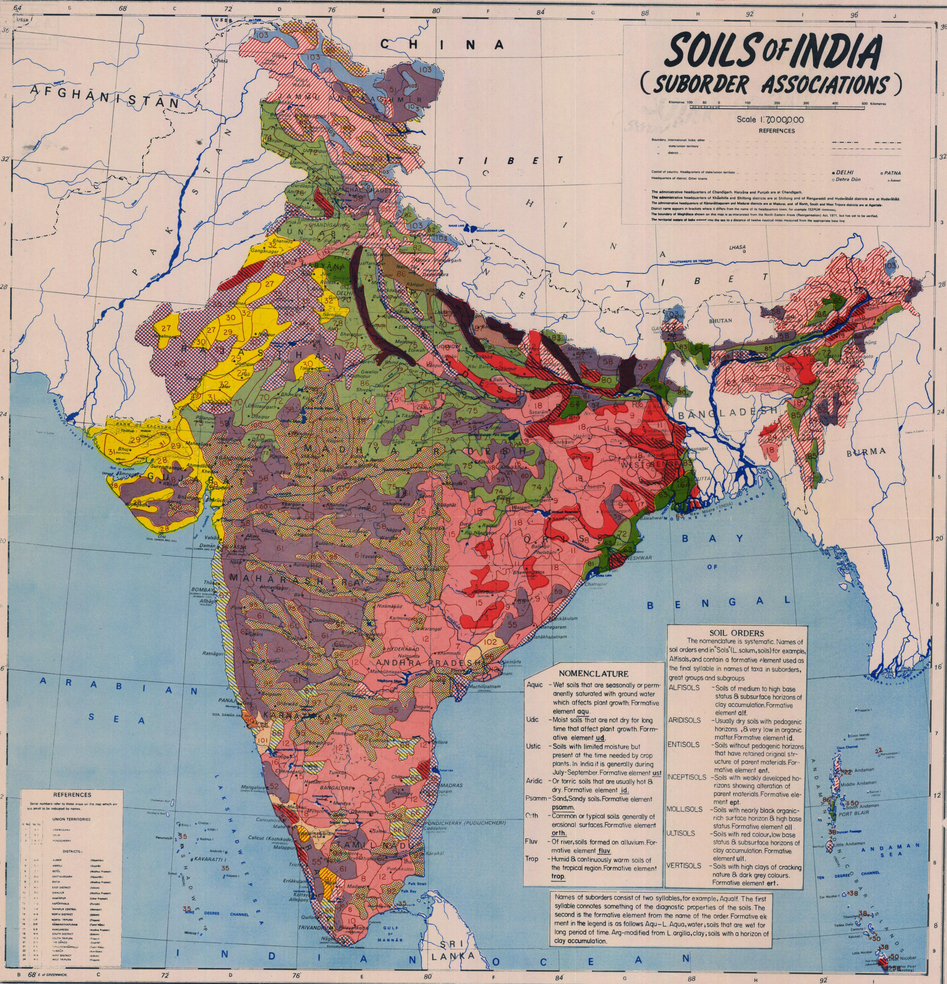
\includegraphics[width=0.9\linewidth]{images/Soiltype-map-of-India.png}
        \end{figure}
        \label{fig:soilmapofindia}
        \tiny \textbf{Figure ~\ref{fig:soilmapofindia} :} European Soil Data Centre (ESDAC)\footnotemark[8].
    \end{columns}
    \footnotetext[8]{Source : \href{https://esdac.jrc.ec.europa.eu}{\url{https://esdac.jrc.ec.europa.eu/}}}
\end{frame}

% TODO:
% \subsection{Elevation as Feedback Breaker}
% \begin{frame}{Elevation Breaks Precipitation-Soil Moisture Feedback}
%     $$When an MD encounters elevation > 900m (Eastern Ghats region), three processes weaken TP-SWVL1 coupling :
%       FIX : update this table vlaues
%     \begin{table}
%     \centering
%     \caption{Elevation and Terrain Characteristics by Track}
%         \begin{tabular}{c|ccccc|c}
%             \hline
%             Track & Mean Elev (m) & Max Slope ($.^\circ$) & Terrain & Duration (h) & Soil Memory & Soil Type \\
%             \hline
%             1 & 600 & 12 & Mountains & 71 & -0.061 & Sand \\
%             2 & 120 & 2 & Plains & 119 & -0.079 & Clay \\
%             3 & 150 & 3 & Plains & 143 & 0.350 & Clay \\
%             4 & 750 & 14 & Mountains & 63 & 0.032 & Sand \\
%             5 & 180 & 4 & Plains & 167 & 0.584 & Clay \\
%             6 & 140 & 2 & Plains & 105 & 0.034 & Clay \\
%             \hline
%         \end{tabular}
%     \end{table}
%
%     \begin{enumerate}
%         \item Orographic Precipitation Efficiency  : Forced ascent produces intense rainfall with high runoff (not infiltration). \cite{clapp1978empirical}
%         \item Drainage Acceleration : Steep slopes ($> 8^\circ$) increase drainage by 2-3 times vs. flat terrain $\rightarrow$ soil doesn't retain moisture
%         \item Reduced Latent Heating : Rapid runoff leaves surface dry -> lower evaporative cooling -> weaker LHF feedback
%     \end{enumerate}
%
%        \begin{itemize}{Prediction :}
%         \item Tracks 1, 4 (Eastern Ghats, elev range 900-1600 m) show shorter duration ($\sim$ $70h$) and weak autocorrelation (< 0.1) despite possible pre-landfall moisture.
%         \item Tracks 2, 3, 5, 6 (Plains, avg. elev $\approx$200 m) show long duration (~130h) and strong autocorrelation (>0.3).
%         \item Plains (tracks 2,3,[5],6) : rainfall $\rightarrow$ infiltration $\rightarrow$ soil moisture $\uparrow$ $\rightarrow$ heat flux $\uparrow$ $\rightarrow$ sustains MD $\rightarrow$ long duration.
%         \item High elevated region/western Ghats (tracks 1,4) : rainfall $\rightarrow$ rapid runoff $\rightarrow$ soil moisture $\downarrow$ $\rightarrow$ heat flux $\downarrow$ $\rightarrow$ md weakens $\rightarrow$ short duration (due to steep slopes \& rapid drainage)
%     \end{itemize}
% \end{frame}

% % TODO: update this BoE chain mechanism
% \subsection{BoE Evidence}
% \begin{frame}{The Brown Ocean Effect : Evidence}
%     \vspace{-0.3cm}
%     \footnotesize
%     \begin{columns}[T]
%         \column{0.52\textwidth}
%         % FIX: update HF values from coupling_metrics_FSI_enhanced.csv
%             % Mean latent HF: -85.9 W/m$^2$ (2024)
%             % Mean sensible HF: -10.3 W/m$^2$
%             % Land phase amplitude: 77.57 W/m$^2$
%             % Ocean phase amplitude: 13.54 W/m$^2$
%         \begin{block}{Supporting Evidence}
%             \begin{itemize}
%                 \item \textbf{Flux Continuity :} Landfall total flux change is only \texttt{+51.2 W/m$^2$}, proving the "moisture cut-off" from Ocean.
%                 \item \textbf{LHF Maintenance :} Post-landfall \texttt{LHF} (\texttt{-82.9 W/m$^2$}) remains the dominant energy driver.
%                 \item \textbf{Diurnal Pumping :} Mean \texttt{SHF} Amplitude is $\approx 4$ times stronger over land, enabling continuous daily convection.
%                 \item \textbf{Lag Dynamics :} Track 5 shows a clear \texttt{+6h} lag (\texttt{SWVL1} $\rightarrow$ \texttt{TP}), proving the soil moisture is providing moisture to atmosphere (MD) via evaporation.
%                 % FIX: chose above or below or mix them
%                 % \item \textbf{Flux Continuity :} Landfall total flux change is only \texttt{+51.2 W/m$^2$}, mitigating the "moisture cut-off."
%                 % \item \textbf{LHF Maintenance :} Post-landfall \texttt{LHF} (\texttt{-82.9 W/m$^2$}) remains the dominant energy driver.
%                 % \item \textbf{Diurnal Pumping :} \texttt{SHF} Amplitude is $\approx 4\times$ stronger over land, fueling daily convection.
%                 % \item \textbf{Lag Dynamics :} Track 5 \texttt{+6h} lag (\texttt{SM} $\rightarrow$ \texttt{TP}) proves the soil is the moisture source.
%             \end{itemize}
%         \end{block}
%
%         \column{0.48\textwidth}
%         \begin{block}{Physical Mechanism}
%             \begin{itemize}
%                 \item \textbf{Pseudo-Ocean over Land :} Clay soils over the Plains act as a "Brown Ocean" reservoir.
%                 \item \textbf{Survival Strategy :} Daytime \texttt{SHF} pulse maintains instability while \texttt{LHF} feeds the core.
%                 \item \textbf{The Feedback Loop :} 
%                     \begin{equation}
%                         \text{\texttt{TP}} \xrightarrow{\text{recharge}} \text{\texttt{SWVL1}} \xrightarrow{\text{flux}} \text{\texttt{LHF}} \xrightarrow{\text{evaporation}} \text{\texttt{TP}}
%                     \end{equation}
%             \end{itemize}
%         \end{block}
%     \end{columns}
%
%     % FIX: values from lag plots
%     % \vspace{-0.3cm}
%     % \begin{center}
%     %     \textbf{Lead-Lag Phase Relationship (Hours)} \\
%     %     \vspace{0.1cm}
%     %     \tiny
%     %     \begin{tabular}{lccccc}
%     %         \toprule
%     %         \textbf{Track ID} & \textbf{Origin} & \texttt{TP} $\rightarrow$ \texttt{SWVL1} & \texttt{SWVL1} $\rightarrow$ \texttt{LHF} & \texttt{LHF} $\rightarrow$ \texttt{TP} & \textbf{Feedback Status} \\
%     %         \midrule
%     %         Track 1 &        & \texttt{+12 to +24 h} & \texttt{None} & \texttt{None} & \textbf{Broken (Eastern Ghats)} \\
%     %         Track 2 &        & \texttt{0 h} & \texttt{+1 h} & \texttt{+3 h} & \textbf{Strong Coupling} \\
%     %         Track 3 &        & \texttt{0 h} & \texttt{+1 h} & \texttt{+2 h} & \textbf{Strong Coupling} \\
%     %         Track 4 &        & \texttt{+12 to +24 h} & \texttt{None} & \texttt{None} & \textbf{Broken (Eastern Ghats)} \\
%     %         Track 5 &        & \texttt{0 h} & \texttt{+2 h} & \texttt{+4 h} & \textbf{Memory Sustained} \\
%     %         Track 6 &        & \texttt{0 h} & \texttt{+1 h} & \texttt{+3 h} & \textbf{Memory Sustained} \\
%     %         \bottomrule
%     %     \end{tabular}
%     % \end{center}
%     % same table as above
%     % \begin{center}
%     %     \textbf{Lead-Lag Relationship (Hours)} \\
%     %     \tiny
%     %     \begin{tabular}{lcccc}
%     %         \toprule
%     %         \textbf{Track Type} & \texttt{TP} $\rightarrow$ \texttt{SM} & \texttt{SM} $\rightarrow$ \texttt{LHF} & \texttt{LHF} $\rightarrow$ \texttt{TP} & \textbf{Status} \\
%     %         \midrule
%     %         Track 3 (Land-Orig) & \texttt{0 h} & \texttt{+1 h} & \texttt{+2 h} & \textbf{Strong Coupling} \\
%     %         Track 5 (Ocean-Orig) & \texttt{0 h} & \texttt{+3 h} & \texttt{+5 h} & \textbf{Memory Sustained} \\
%     %         Track 1 (Coastal) & \texttt{+24 h} & \texttt{None} & \texttt{None} & \textbf{Broken Feedback} \\
%     %         \bottomrule
%     %     \end{tabular}
%     % \end{center}
%
%     \footnotesize
%     \begin{itemize}
%         \item \textbf{Loop Break (1, 4) :} Topographic runoff (Eastern Ghats) breaks the feedback loop by draining the moisture before the loop can begin. \cite{clapp1978empirical}
%         \item \textbf{Closed Loop (2, 3, 5) :} Moisture cycles from surface to core within a single diurnal cycle, sustaining the MD (from rain to soil to flux.). Uses high soil memory to buffer decay after slowdown. Avoids terrain/elevation runoff.
%     \end{itemize}
%
%     \vspace{0.3}
%     \footnotesize
%     \textbf{The Brown Ocean is a geography dependent :} Survival of low-pressure mesoscale systems depends on hitting the soil type (Plains/Clay) where soil moisture can effectively replace the ocean-driven system. With the condition, MD survive or avoid high elevation of steep Eastern Ghats.
% \end{frame}
%
% \begin{frame}{Why Track 5 Succeeded When 1 \& 4 Failed}
%     \footnotesize
%     \begin{columns}[T]
%         \column{0.32\textwidth}
%         \begin{block}{Track 1 (Failed)}
%             \begin{itemize}\scriptsize
%                 \item \textbf{Path :} Ocean $\rightarrow$ Eastern Ghats
%                 \item \textbf{Soil Type :} Sandy / Rock
%                 \item \textbf{Capacity :} \texttt{0.140} (Low)
%                 \item \textbf{Feedback :} \texttt{-0.092} (Negative)
%                 \item \textbf{Lag :} \texttt{-24h} (Runoff)
%                 \item \textbf{Duration :} \texttt{75h}
%             \end{itemize}
%         \end{block}
%
%         \column{0.32\textwidth}
%         \begin{block}{Track 4 (Failed)}
%             \begin{itemize}\scriptsize
%                 \item \textbf{Path :} Ocean $\rightarrow$ Sandy Coast
%                 \item \textbf{Soil Type :} Sandy Loam
%                 \item \textbf{Capacity :} \texttt{0.178} (Low)
%                 \item \textbf{Feedback :} \texttt{-0.197} (Negative)
%                 \item \textbf{Lag :} \texttt{None} (Broken)
%                 \item \textbf{Duration :} \texttt{65h}
%             \end{itemize}
%         \end{block}
%
%         \column{0.32\textwidth}
%         \begin{block}{Track 5 (Success)}
%             \begin{itemize}\scriptsize
%                 \item \textbf{Path :} Ocean $\rightarrow$ IG Plains
%                 \item \textbf{Soil Type :} \textbf{Clay / Silt}
%                 \item \textbf{Capacity :} \textbf{\texttt{0.270}} (High)
%                 \item \textbf{Feedback :} \texttt{+0.525} (\textbf{Strong})
%                 \item \textbf{Lag :} \texttt{+6h} (\texttt{SM} $\rightarrow$ \texttt{TP})
%                 \item \textbf{Duration :} \texttt{163h}
%             \end{itemize}
%         \end{block}
%     \end{columns}
%
%     \vspace{0.2cm}
%     \begin{block}{The "Brown Ocean" Threshold}
%         \textbf{Criteria for MD Survival after Landfall :}
%         \begin{enumerate}
%             \item \textbf{Inland Corridor :} Must reach Indo-Gangetic (IG) Clay soils to sustain \texttt{LHF}.
%             \item \textbf{Memory Threshold :} Soil Moisture \texttt{ACF-24h} must remain non-negative.
%             \item \textbf{Coupling Efficiency :} SM must lead Precipitation (\texttt{Lag $>0$}) or be synchronous.
%         \end{enumerate}
%     \end{block}
% \end{frame}
%
% % TODO: check this
% \begin{frame}{Synthesis: Two-Level Control Mechanism}
%     \footnotesize
%     \begin{block}{Level 1: Soil Type (Capacity)}
%         \centering
%         \begin{tabular}{lcc}
%             \toprule
%             \textbf{Region Type} & \textbf{Mean Duration} & \textbf{Soil Texture}          \\
%             \midrule
%             Coastal (1, 4)       & \texttt{76h}                    & Sandy (low moisture retention) \\
%             Plains (2, 3, 5, 6)  & \texttt{135h}                   & Clay (high moisture retention) \\
%             \bottomrule
%         \end{tabular}
%     \end{block}
%
%     \vspace{0.3cm}
%     \footnotesize
%     \begin{block}{Level 2: Antecedent Soil Moisture (24 hours before landfall) \& Coupling (Fuel + Efficiency)}
%         \begin{itemize}
%             \item Pre-landfall SWVL1 (Soil moisture/soil water content) enables initial feedback
%             \item TP-SWVL1 coupling strength determines sustainability
%             \item FSI + diurnal amplitude predict longevity threshold
%         \end{itemize}
%     \end{block}
%
%     \vspace{0.3cm}
%     \footnotesize
%     Track 5 (anomaly) suggests additional factors (moisture advection, surviving Eastern Ghats elevation mechanism and efficient soil moisture extraction from land to sustainability, unlike track 1 and 4).
% \end{frame}
%
% \begin{frame}[label=twolevelmechanism]{Two-Level Control Mechanism}
%     \footnotesize
%     \begin{block}{Level 1: Geographical Constraint}
%         \centering
%         \begin{tabular}{lccc}
%             \toprule
%             \textbf{Tracks} & \textbf{Mean Dur.} & \textbf{Primary Constraint} & Terrain \\
%             \midrule
%             1, 4   & \texttt{70h} & Steep terrain, Rapid Runoff (Low Capacity) & Eastern Ghat (Elevation \texttt{900-1400 m})\\
%             2, 3, 5, 6 & \texttt{142h} & Clay-Rich, High Water Retention (High Capacity) & Indo-Gangetic plains (Elevation \texttt{< 200 m}) \\
%             \bottomrule
%         \end{tabular}
%
%         \vspace{0.2cm}
%         \begin{itemize}
%             \item Geographicaly MDs that hit the Indo-Gangetic Plains live \textbf{twice as long} as those hitting the Eastern Ghats/Coastal sands. 
%
%                 (this might be over generalisation? need more data for analysis. TODO: analysis for 2023 to 2025)
%         \end{itemize}
%     \end{block}
%
%     \vspace{0.2cm}
%     \begin{block}{Level 2: Dynamic Feedback}
%         \begin{itemize}
%             \item \textbf{Antecedent SM :} Sets the initial state \texttt{24h} before landfall.
%             \item \textbf{Coupling Efficiency (CE) :} Determines if the feedback (\texttt{TP} $\leftrightarrow$ \texttt{SWVL1}) is fast enough to sustain the vortex core within a diurnal cycle.
%             \item \textbf{Diurnal SHF Amplitude :} Triggers daily convection.
%         \end{itemize}
%     \end{block}
%
%     \vspace{0.2cm}
%     \begin{exampleblock}{The Track 5 Insight}
%         Track 5 isn't an anomaly; it proves that \textbf{Capacity > Origin}. Despite originating in the Ocean, it survived 165h because it reached the Clay soil ("Brown Ocean") of the Plains.
%     \end{exampleblock}
% \end{frame}
%
% \subsection{\texttt{MODIS} Satellite Image Interpretation}
% \begin{frame}{Structural Asymmetry : Southwest Quadrant of MD Tracks Convection}
%     \begin{columns}[T]
%         \column{0.5\textwidth}
%         \footnotesize
%         \begin{block}{Observation : Southwest Cloud Cluster}
%             \footnotesize
%             \begin{itemize}
%                 \item \texttt{MODIS} composites show maximum cloud density in the \textbf{southwest (left-forward)} quadrant relative to the fast moving tracks.
%                 \item The right (northeast) side remains relatively clear or has thinner clouds.
%             \end{itemize}
%         \end{block}
%
%         \column{0.5\textwidth}
%         % TODO: Add literature support and cite this mechanism
%         \footnotesize
%         \begin{block}{Physical Mechanism}
%             \footnotesize
%             \begin{itemize}
%                 \item \textbf{Low-Level Jet (LLJ) Coupling:} Cyclonic winds on the southern flank align with the monsoon LLJ, maximizing moisture convergence.
%                 \item \textbf{Vertical Wind Shear:} Strong easterly shear "tilts" the vortex, forcing upward motion and deep convection to the west of the center.
%             \end{itemize}
%         \end{block}
%     \end{columns}
%
%     \vspace{0.5cm}
%     \tiny \textit{Note the cloud cluster follows the moisture influx from the BOB.}
% \end{frame}

%%%%% Previus years MD detections %%%%
% \subsubsection{MD detection for 2019}
% \begin{frame}[label=tracks2021]{MD Tracks (June-September 2019)}
% 	\vspace{-0.3cm}
% 	\begin{center}
% 		\begin{columns}[T, onlytextwidth]
% 			\column{0.49\textwidth}
% 			\vspace{-0.2cm}
% 			\begin{center}
% 				\begin{figure}
% 					\includegraphics[width=1.1\linewidth]{../version21-with-no-ocean-masking/output_2019/MD_track_2019.png}
% 				\end{figure}
% 				\footnotesize Detected MD tracks using ERA5 single level Dataset (2020)
% 			\end{center}
%
% 			\column{0.49\textwidth}
% 			\vspace{-0.6cm}
% 			\begin{center}
% 				\begin{figure}
% 					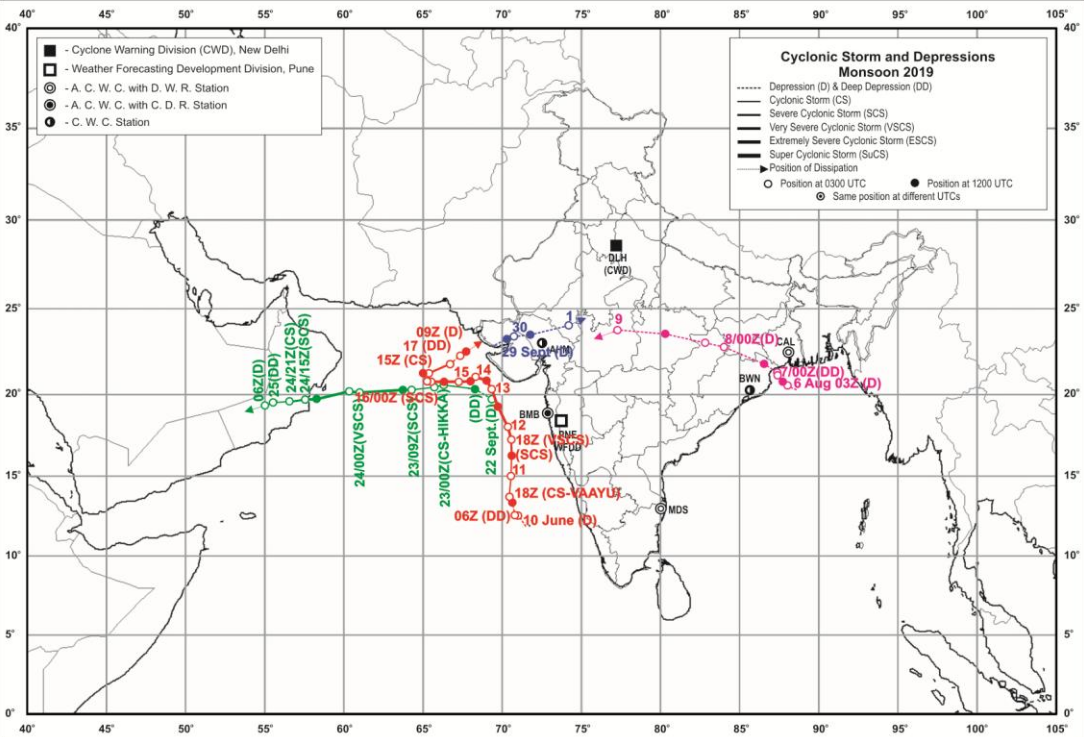
\includegraphics[width=1.1\linewidth, height=0.74\textheight]{images/IMD-report-2019.png}
% 					% 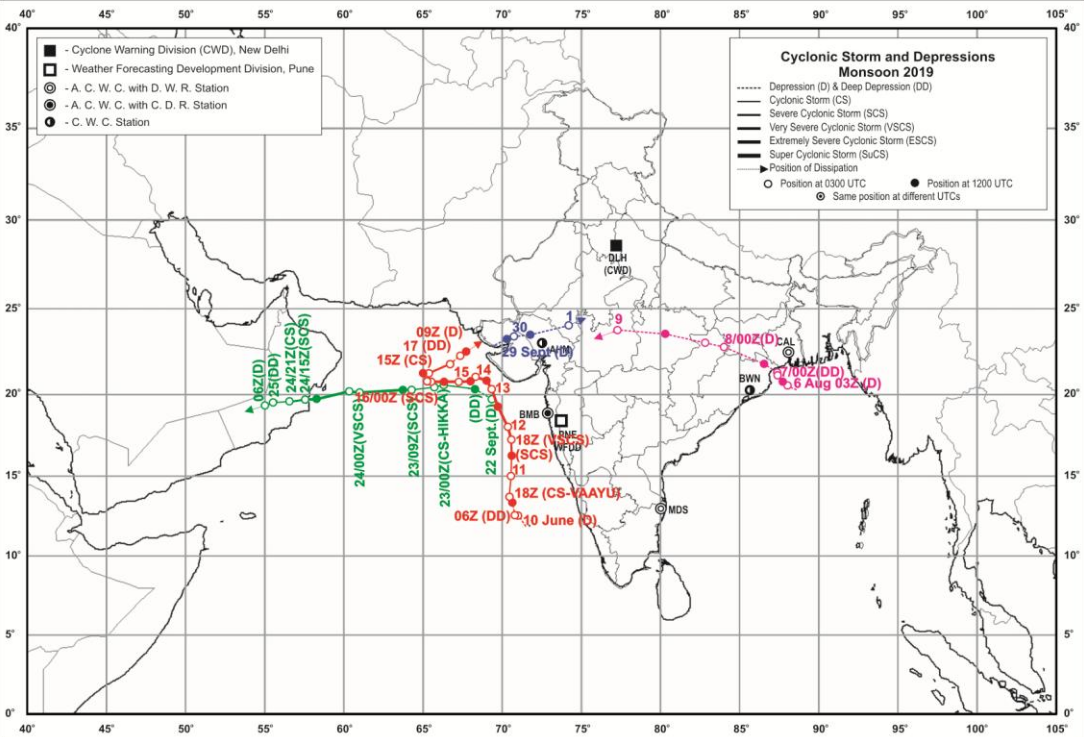
\includegraphics[width=1.12\linewidth, height=0.5\textheight, keepaspectratio]{images/IMD-report-2019.png}
% 				\end{figure}
% 				\footnotesize IMD Annual Monsoon report 2021 \footnotemark[10]
% 			\end{center}
% 		\end{columns}
%
% 		\vspace{-0.6cm}
% 		\footnotetext[10]{\tiny Source : IMD Annual Monsoon Report 2019 (page 17) \href{https://mausam.imd.gov.in/shimla/mcdata/monsoon/images/2019/monsoon\_report\_2019.pdf}{\url{https://mausam.imd.gov.in/shimla/mcdata/monsoon/images/2019/monsoon\_report\_2019.pdf}}}
% 	\end{center}
% \end{frame}
%
% \subsubsection{MD detection for 2020}
% \begin{frame}[label=tracks2021]{MD Tracks (June-September 2020)}
% 	\vspace{-0.3cm}
% 	\begin{center}
% 		\begin{columns}[T, onlytextwidth]
% 			\column{0.49\textwidth}
% 			\vspace{-0.2cm}
% 			\begin{center}
% 				\begin{figure}
% 					\includegraphics[width=1.1\linewidth]{../version21-with-no-ocean-masking/output_2020/MD_track_2020.png}
% 				\end{figure}
% 				\footnotesize Detected MD tracks using ERA5 single level Dataset (2020)
% 			\end{center}
%
% 			\column{0.49\textwidth}
% 			\vspace{-0.6cm}
% 			\begin{center}
% 				\begin{figure}
% 					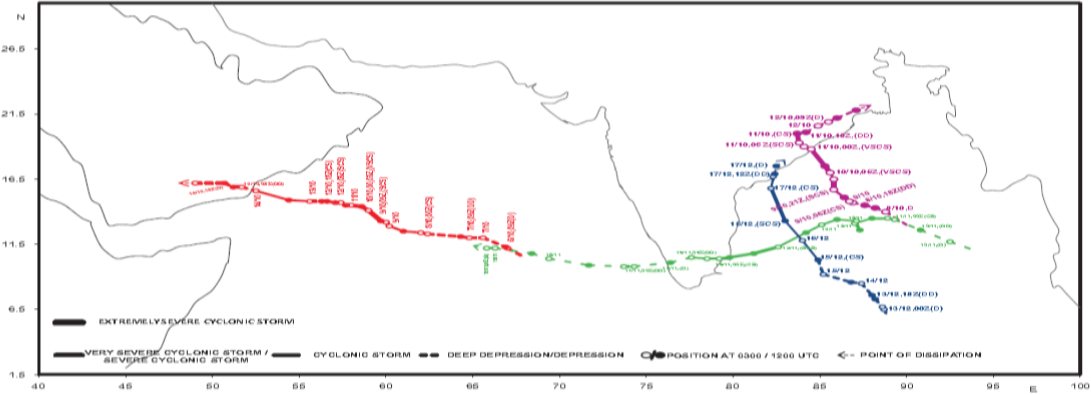
\includegraphics[width=\linewidth, height=0.74\textheight]{images/IMD-report-2020.png}
% 					% 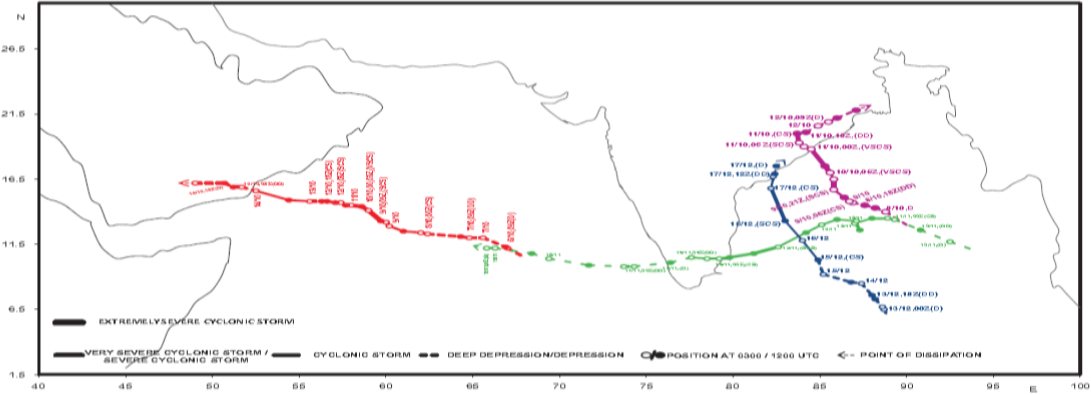
\includegraphics[width=1.12\linewidth, height=0.5\textheight, keepaspectratio]{images/IMD-report-2020.png}
% 				\end{figure}
% 				\footnotesize IMD Annual Monsoon report 2020 \footnotemark[10]
% 			\end{center}
% 		\end{columns}
%
% 		\vspace{-0.6cm}
% 		% \footnotetext[10]{\tiny Source : IMD Annual Monsoon Report 2020 (page 7) \href{https://rsmcnewdelhi.imd.gov.in/report.php?internal\_menu=MzQ=}{\url{https://rsmcnewdelhi.imd.gov.in/report.php?internal\_menu=MzQ=}}}
% 		% \footnotetext[10]{\tiny Source : IMD Annual Monsoon Report 2020 (page 13) \href{https://internal.imd.gov.in/press_release/20201220_pr_963.pdf}{\url{https://internal.imd.gov.in/press_release/20201220_pr_963.pdf}}}
% 		\footnotetext[11]{\tiny Source : IMD Annual Monsoon Report 2020 (page 13) \href{https://mausam.imd.gov.in/imd_latest/contents/ar2020.pdf}{\url{https://mausam.imd.gov.in/imd_latest/contents/ar2020.pdf}}}
%
% 	\end{center}
% \end{frame}
%
% \subsubsection{MD detection for 2021}
% \begin{frame}[label=tracks2021]{MD Tracks (June-September 2021)}
% 	\vspace{-0.3cm}
% 	\begin{center}
% 		\begin{columns}[T, onlytextwidth]
% 			\column{0.49\textwidth}
% 			\vspace{-0.2cm}
% 			\begin{center}
% 				\begin{figure}
% 					\includegraphics[width=1.1\linewidth]{../version21-with-no-ocean-masking/output_2021/MD_track_2021.png}
% 				\end{figure}
% 				\footnotesize Detected MD tracks using ERA5 single level Dataset (2021)
% 			\end{center}
%
% 			\column{0.49\textwidth}
% 			\vspace{-0.5cm}
% 			\begin{center}
% 				\begin{figure}
% 					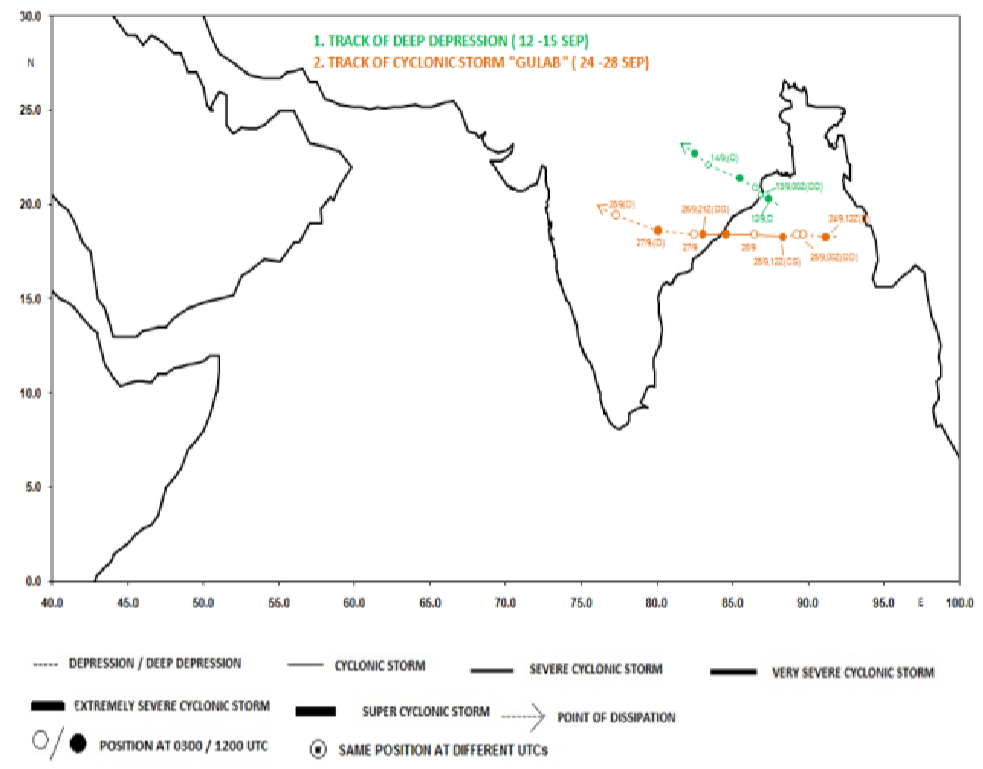
\includegraphics[width=\linewidth, height=0.74\textheight]{images/IMD-report-2021.png}
% 					% 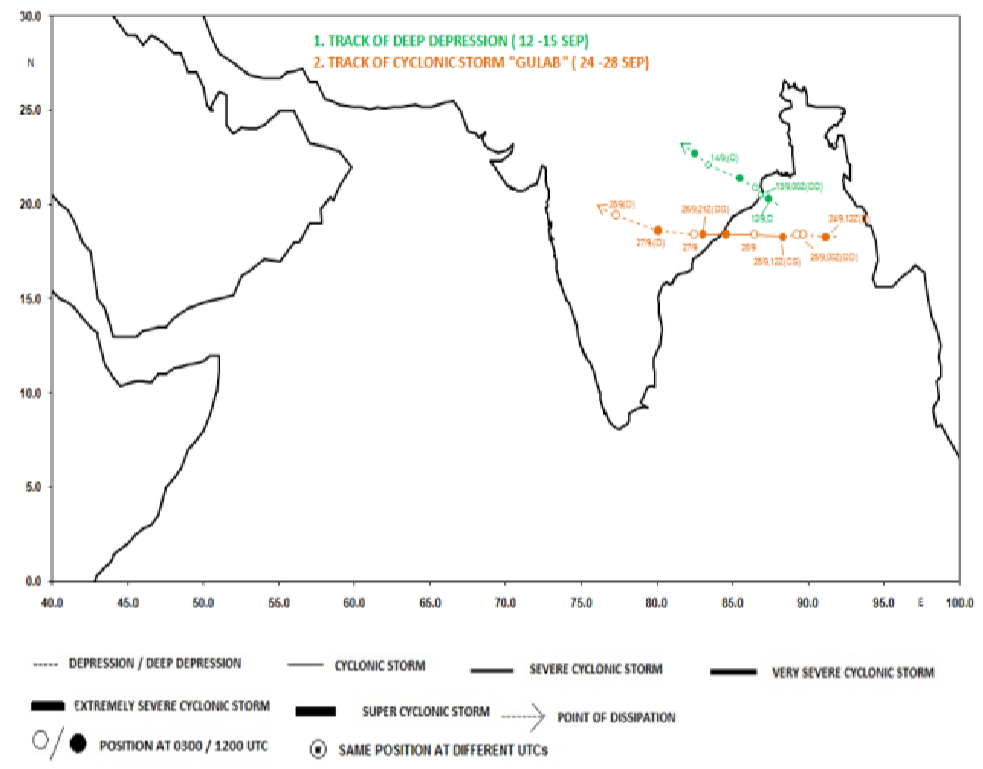
\includegraphics[width=1.12\linewidth, height=0.5\textheight, keepaspectratio]{images/IMD-report-2021.png}
% 				\end{figure}
% 				\footnotesize IMD Annual Monsoon report 2021 \footnotemark[10]
% 			\end{center}
% 		\end{columns}
%
% 		\vspace{-0.6cm}
% 		\footnotetext[12]{\tiny Source : IMD Annual Monsoon Report 2021 (page 30) \href{https://mausam.imd.gov.in/imd\_latest/contents/ar2021.pdf}{\url{https://mausam.imd.gov.in/imd\_latest/contents/ar2021.pdf}}}
% 	\end{center}
% \end{frame}
%
% \subsubsection{MD detection for 2022}
% \begin{frame}[label=tracks2022]{MD Tracks (June-September 2022)}
% 	\vspace{-0.3cm}
% 	\begin{center}
% 		\begin{columns}[T, onlytextwidth]
% 			\column{0.49\textwidth}
% 			\begin{center}
% 				\vspace{-0.2cm}
% 				\begin{figure}
% 					\includegraphics[width=1.1\linewidth]{../version21-with-no-ocean-masking/output_2022/MD_track_2022.png}
% 				\end{figure}
% 				\footnotesize Detected MD tracks using ERA5 single level Dataset (2022)
% 			\end{center}
%
% 			\column{0.49\textwidth}
% 			\vspace{-0.5cm}
% 			\begin{center}
% 				\begin{figure}
% 					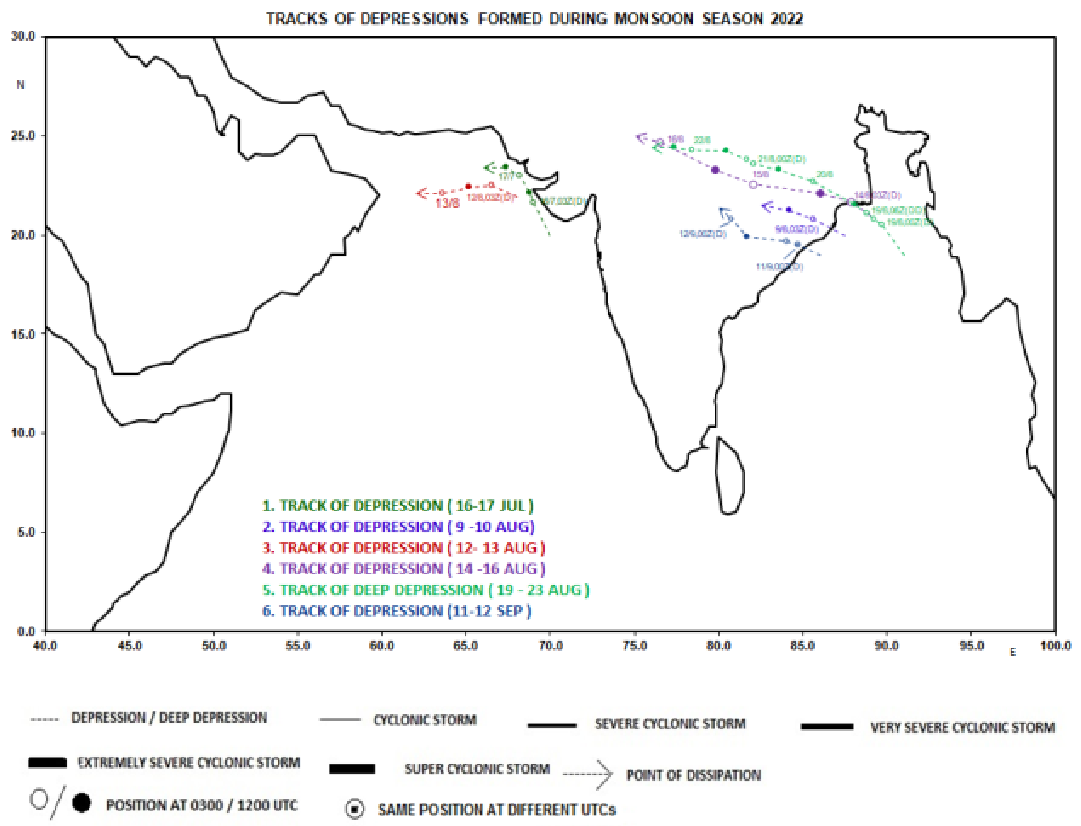
\includegraphics[width=\linewidth, height=0.74\textheight]{images/IMD-report-2022.png}
% 					% 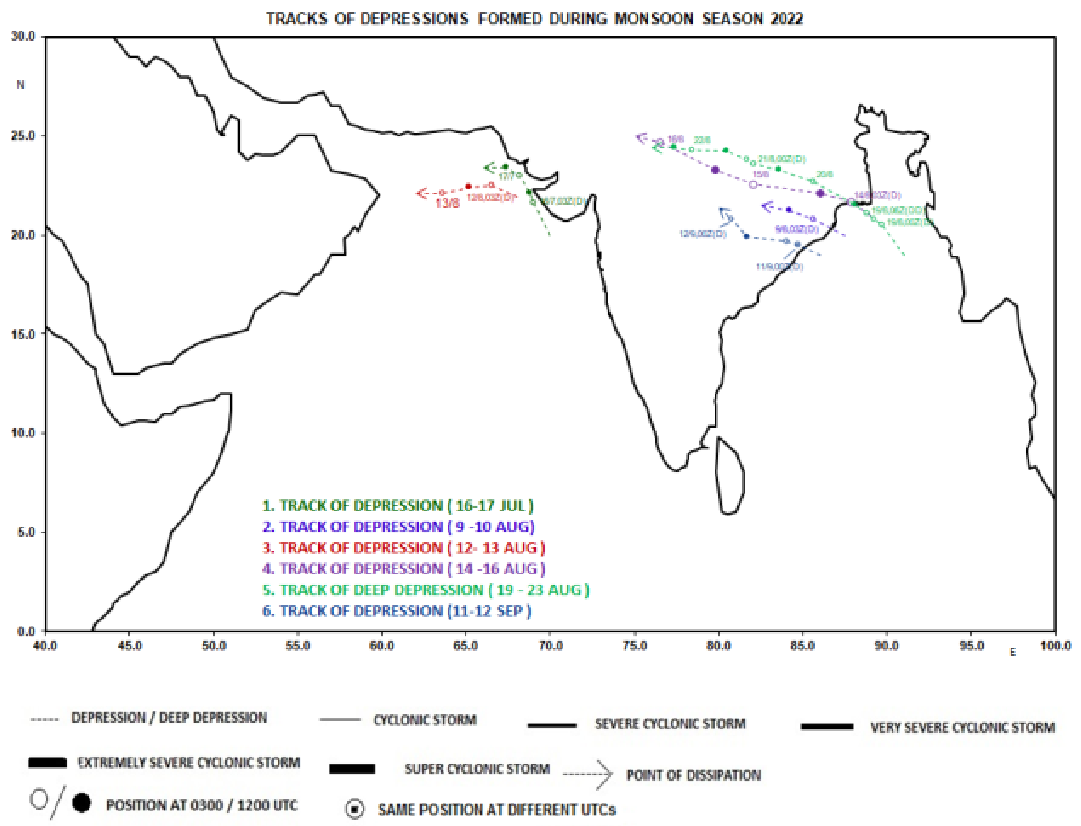
\includegraphics[width=1.12\linewidth, height=0.5\textheight, keepaspectratio]{images/IMD-report-2022.png}
% 				\end{figure}
% 				\footnotesize IMD Annual Monsoon report 2022 \footnotemark[10]
% 			\end{center}
% 		\end{columns}
%
% 		\vspace{-0.7cm}
% 		\footnotetext[13]{\tiny Source : IMD Annual Monsoon Report 2022 (page 29) \href{https://mausam.imd.gov.in/imd\_latest/contents/ar2022.pdf}{\url{https://mausam.imd.gov.in/imd\_latest/contents/ar2022.pdf}}}
% 	\end{center}
% \end{frame}
%
% \subsubsection{MD detection for 2023}
% \begin{frame}[label=tracks2023]{MD Tracks (June-September 2023)}
% 	\vspace{-0.3cm}
% 	\begin{center}
% 		\begin{columns}[T, onlytextwidth]
% 			\column{0.49\textwidth}
% 			\vspace{-0.2cm}
% 			\begin{center}
% 				\begin{figure}
% 					\includegraphics[width=1.1\linewidth]{../version21-with-no-ocean-masking/output_2023/MD_track_2023.png}
% 				\end{figure}
% 				\footnotesize Detected MD tracks using ERA5 single level Dataset (2023)
% 			\end{center}
%
% 			\column{0.49\textwidth}
% 			\vspace{-0.5cm}
% 			\begin{center}
% 				\begin{figure}
% 					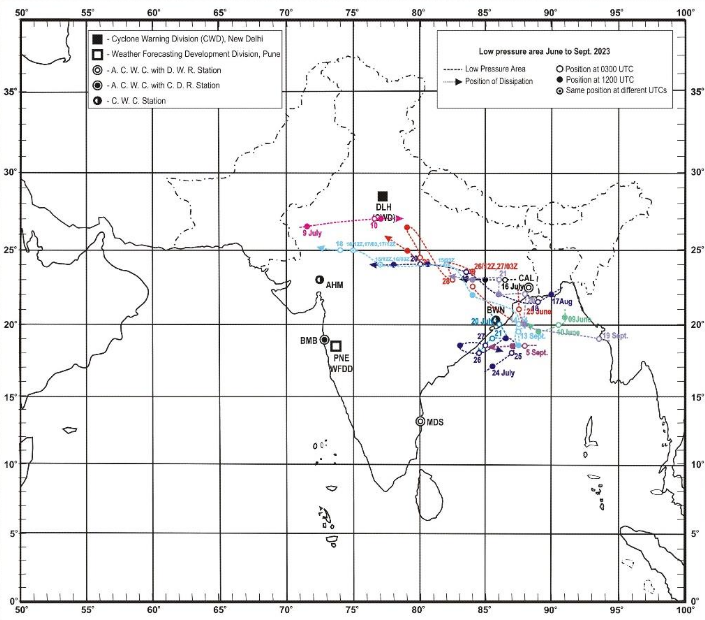
\includegraphics[width=1.1\linewidth, height=0.74\textheight]{images/IMD-report-2023.png}
% 					% 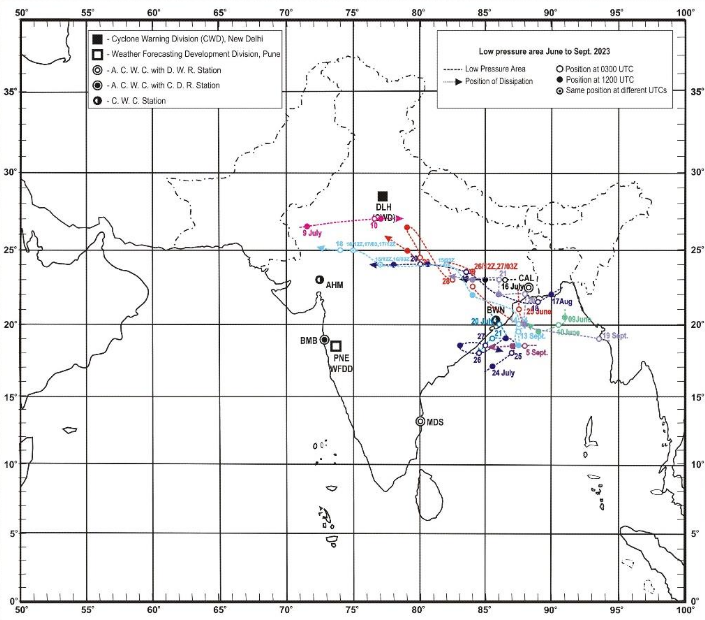
\includegraphics[width=1.12\linewidth, height=0.5\textheight, keepaspectratio]{images/IMD-report-2023.png}
% 				\end{figure}
% 				\footnotesize IMD Annual Monsoon report 2023 \footnotemark[10]
% 			\end{center}
% 		\end{columns}
%
% 		\vspace{-0.6cm}
% 		\footnotetext[14]{\tiny Source : IMD Annual Monsoon Report 2023 (page 23) \href{https://internal.imd.gov.in/press\_release/20231001\_pr\_2555.pdf}{\url{https://internal.imd.gov.in/press\_release/20231001\_pr\_2555.pdf}}}
% 	\end{center}
% \end{frame}
%
% \subsubsection{MD detection for 2025}
% \begin{frame}[label=tracks2025]{MD Tracks (June-September 2025)}
% 	\vspace{-0.3cm}
% 	\begin{center}
% 		\begin{columns}[T, onlytextwidth]
% 			\column{0.49\textwidth}
% 			\vspace{-0.2cm}
% 			\begin{center}
% 				\begin{figure}
% 					\includegraphics[width=1.1\linewidth]{../version21-with-no-ocean-masking/output_2025/MD_track_2025.png}
% 				\end{figure}
% 				\footnotesize Detected MD tracks using ERA5 single level Dataset (2025)
% 			\end{center}
%
% 			\column{0.49\textwidth}
% 			\vspace{-0.5cm}
% 			\begin{center}
% 				\begin{figure}
% 					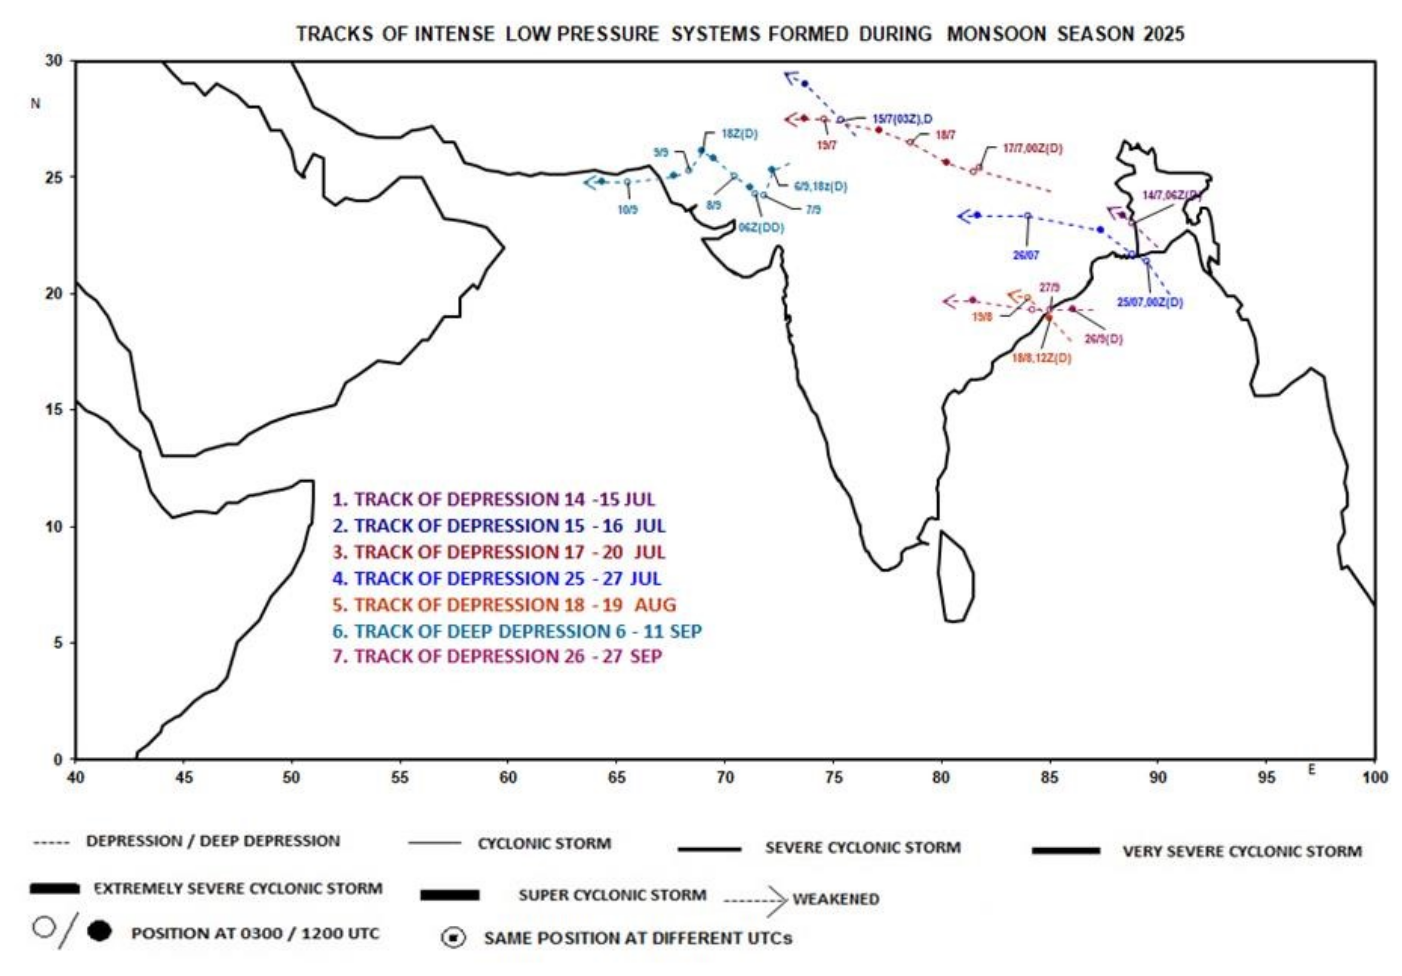
\includegraphics[width=\linewidth, height=0.74\textheight]{images/IMD-report-2025.png}
% 					% 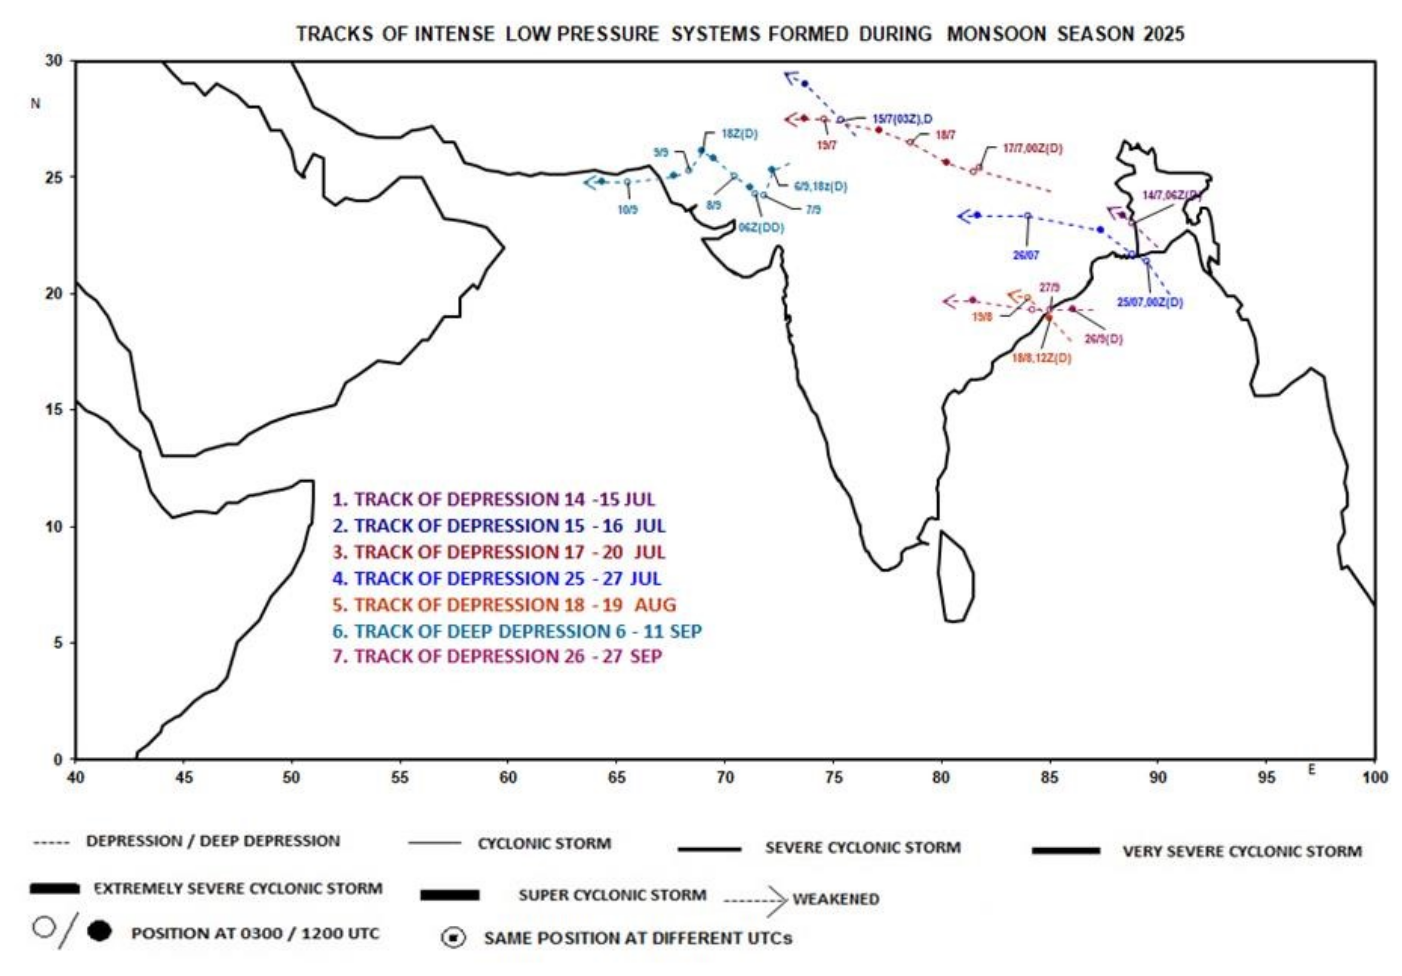
\includegraphics[width=1.12\linewidth, height=0.5\textheight, keepaspectratio]{images/IMD-report-2025.png}
% 				\end{figure}
% 				\footnotesize IMD Annual Monsoon report 2025 \footnotemark[10]
% 			\end{center}
% 		\end{columns}
%
% 		\vspace{-0.6cm}
% 		\footnotetext[15]{\tiny Source : IMD Annual Monsoon Report 2025 (page 7) \href{https://mausam.imd.gov.in/newdelhi/archive/2025-12-13/press\_release\_en.pdf}{\url{https://mausam.imd.gov.in/newdelhi/archive/2025-12-13/press\_release\_en.pdf}}}
% 	\end{center}
% \end{frame}

% \section{Proposed Hypotheses}
% \begin{frame}[plain, noframenumbering]
	\begin{center}
		\Huge \textcolor{blue}{\textbf{Proposed Hypotheses}} \\
	\end{center}
\end{frame}

\subsection{Hypothesis 1}
\begin{frame}{Hypothesis 1 : The Moisture-Recycling Efficiency [1/2]}
	\vspace{-0.1cm}
	\begin{block}{The longevity of an MD depends on the phase-locking of the \texttt{TP-SWVL1-LHF} loop. Long-lived systems exhibit positive lags and high soil memory, whereas short-lived systems are dominated by runoff and negative lags}\end{block}

	\vspace{0.15cm}
	\footnotesize
	\textbf{Statement :} Longevity depends on the synchrony (optimal $0 \pm 6$ h, FSI $>0.4$) of the \texttt{TP-SWVL1-LHF} feedback loop. Long-lived MDs ($\ge 96$h) maintain surface energy exchange through continuous moisture recycling. Short-lived systems ($< 96$h) undergo rapid decay as land-surface friction and moisture depletion collapse the vortex core.

	\vspace{0.2cm}
	\footnotesize
	Longevity is proportional to the strength and sign of the \textbf{Land-Atmosphere Coupling}. Positive feedback (\texttt{TP}$\uparrow \rightarrow$\texttt{SWVL1}$\uparrow \rightarrow$ \texttt{LHF}$\uparrow \rightarrow$ Convection$\uparrow$) creates a \textbf{"Secondary Pseudo-Ocean"} effect. \cite{hunt2017effect}

	\vspace{0.2cm}
	\footnotesize
	\textbf{The Feedback Loop :}
	\[ \text{(\textbf{Precipitation})} \rightarrow \text{(\textbf{Infiltration})} \rightarrow \text{(\textbf{Elevated Soil Moisture})} \rightarrow \text{(\textbf{Sustained \texttt{LHF}})} \rightarrow \text{(\textbf{MD Persistence})} \]

	\vspace{0.2cm}
	\footnotesize
	\textbf{Loop Failure (Tracks 1 \& 4) :}
	\begin{itemize}
		\item \textbf{Broken Lags (\texttt{> 12h}) :} Indicates \textbf{Topographic Runoff} (Eastern Ghats) or \textbf{Saturation Excess} (Sandy Coast).
		\item \textbf{Negative Memory (\texttt{ACF $\approx -0.15$}) :} Prevents the soil from "storing" the energy recharge from precipitation.
	\end{itemize}
\end{frame}

\begin{frame}{Hypothesis 1 : The Moisture-Recycling Efficiency [2/2]}
	\footnotesize
	\textbf{Evidence (Multi-Metric Validation) :}
	\begin{itemize}
		\item \textbf{Brown Ocean dominated Long-lived tracks (2,3,5,6) :} Mean FSI = \textbf{0.42}; Mean ACF = \textbf{0.44}.
		\item \textbf{Runoff dominated Short-lived tracks (1,4) :} Mean FSI = \textbf{0.07}; Mean ACF = \textbf{-0.06}.
	\end{itemize}

	\vspace{0.1cm}
	\begin{center}
		\begin{tabular}{lcccc}
			\toprule
			\textbf{Track} & \textbf{TP-SM Lag} & \textbf{ACF-24h} & \textbf{Coupling}    & \textbf{Duration} \\
			\midrule
			1              & $-6h$              & $-0.061$         & Negative             & 75h               \\
			4              & $-12h$             & $0.032$          & Negative             & 65h               \\
			2, 3, 6        & $0$ to $+3h$       & $0.35-0.45$      & \textbf{Positive}    & 105-124h          \\
			5              & $+6h$              & $0.584$          & \textbf{Very Strong} & 163h              \\
			\bottomrule
		\end{tabular}
	\end{center}

	\vspace{0.1cm}
	\footnotesize
	\textbf{Interpretation :}
	\begin{itemize}
		\item \textbf{Positive Lag \& High ACF (Track 5) :} Soil moisture "leads" the system; high memory creates a self-sustaining survival strategy.
		\item \textbf{Zero Lag \& Moderate ACF (2,3,6) :} Efficient feedback where rainfall immediately recharges the moisture source.  \cite{osuri2020}
		\item \textbf{Negative Lag \& Low ACF (1,4) :} Rainfall does not translate to sustained soil moisture; energy source collapses post-landfall.
	\end{itemize}
\end{frame}

\subsection{Hypothesis 2}
\begin{frame}{Hypothesis 2 : Landfall Energy Budget Transition [1/2]}
	\vspace{-0.1cm}
	\begin{block}{The ocean-to-land transition creates an abrupt "Energy Gap" where MD survival depends on the land's ability to switch from a \texttt{LHF} dominant region to a Diurnal \texttt{SHF} amplified region}\end{block}

	\vspace{0.15cm}
	\footnotesize
	\textbf{Statement :} The ocean-to-land transition produces a significant reduction in surface evaporative cooling ($\Delta$THF $\approx +62.4$ W/m$^2$)\footnotemark[7]. Survival is governed by whether \textbf{Antecedent Soil Moisture} can buffer this large reduction in energy and sustain the core through enhanced sensible heating.
	% TODO:  Literature support : [Coupling between Land–Ocean–Atmosphere and Pronounced Changes in Atmospheric/Meteorological Parameters Associated with the Hudhud Cyclone of October 2014](https://pmc.ncbi.nlm.nih.gov/articles/PMC6313703/) and [Influence of Land Cover and Soil Moisture based Brown Ocean Effect on an Extreme Rainfall Event](https://www.nature.com/articles/s41598-019-53031-6)

	\vspace{0.2cm}
	\footnotesize
	$\Rightarrow$ \textbf{Landfall Signature :} \texttt{LHF}$\downarrow$ magnitude collapses while \texttt{SHF}$\uparrow$ becomes the diurnal engine. (Matches case study by \cite{andersen2014insights} but for Tropical Cyclone)

	\vspace{0.2cm}
	\footnotesize
	\textbf{The Transition Mechanism (energy shift happens via 2 level mechanism) :}
	\begin{enumerate}
		\item \textbf{Latent Collapse :} \texttt{THF} uptake drops sharply as the infinite moisture reservoir (Ocean) is cut-off. The system must immediately rely on stored terrestrial moisture (\texttt{SWVL1}).
		\item \textbf{Sensible Heating :} A transition from negative \texttt{SHF} over ocean ($-9.16$ W/m$^2$)\footnotemark[6] to positive \texttt{SHF} over land ($+4.50$ W/m$^2$)\footnotemark[6] provides the \textbf{diurnal instability} required for inland maintenance.
	\end{enumerate}

	% FIX:  Doesn't match in expampleblock
	% Track 1: Before -132.9 -> After -97.2 = +35.7 W/m$^2$
	% Track 4: Before -155.4 -> After -96.8 = +58.7 W/m$^2$
	% Track 5: Before -135.0 -> After -80.9 = +54.1 W/m$^2$
	\vspace{0.2cm}
	\begin{exampleblock}{\footnotesize The Spike or "Shock" Metric in the Heat flux change}
		\footnotesize Observed landfall flux transition : Magnitude change of (\textbf{$+68.8$ W/m$^2$})\footnotemark[6] (Before: $-153.6$ $\rightarrow$ After: $-84.8$ W/m$^2$).
	\end{exampleblock}

	\footnotetext[6]{Mean values are derived for Ocean-Origin tracks (1, 4 and 5), Land-Origin tracks have no values over ocean.}
	\footnotetext[7]{Upward energy supply from the surface has decreased by that amount.}
\end{frame}

\begin{frame}{Hypothesis 2 : Landfall Energy Budget Transition [2/2]}
	\footnotesize
	\textbf{Evidence (Survival vs. Dissipation Strategies) :}
	\begin{itemize}
		\item \textbf{Ocean-Origin Short-lived (Tracks 1, 4) :}
		      \begin{itemize}\footnotesize
			      \item \textbf{The Shock :} \texttt{THF} magnitude dropped by \textbf{\texttt{+41} to \texttt{+65 W/m$^2$}} after landfall. \cite{nair2011influence}
			      \item \textbf{The Failure :} Low soil capacity and Negative memory (\texttt{ACF < 0}) prevent the land from compensating for the loss of ocean evaporation. "Energy Gap" could not be filled; core moisture starved within \texttt{$\approx$70h}.
		      \end{itemize}
		\item \textbf{Ocean-Origin Long-lived (Track 5 - The Buffer) :}
		      \begin{itemize}\footnotesize
			      \item \textbf{The Shock :} Experienced the \textbf{largest} landfall shift (\texttt{$+70.5$ W/m$^2$}).
			      \item \textbf{Result :} High \textbf{Soil Moisture Memory (\texttt{ACF = 0.584})} acted as a thermodynamic buffer, sustaining the vortex until it reached the Indo-Gangetic Plain "Brown Ocean." This "Energy Gap" could be filled; thus core moisture sustained for \texttt{$\approx$163h}, despite a massive drop in immediate flux magnitude \texttt{$\Delta$ THF = +70.5 W/m$^2$} (Before landfall \texttt{$\approx$-155.3  W/m$^2$ $\rightarrow$ $\approx$-84.8 W/m$^2$} after landfall, \scriptsize 70.5 units closer to zero\footnotesize). \cite{nair2011influence}
		      \end{itemize}
		\item \textbf{Land-Origin Long-lived (Tracks 2, 3, 6) :}
		      \begin{itemize}\footnotesize
			      \item No discrete landfall shock; energy derived entirely from terrestrial recycling (\texttt{ACF-24h}). \cite{chang2009}
			      \item Represents the theoretical upper limit of coupling efficiency (\texttt{CE=15.35}) where land mimics ocean. \cite{hunt2017effect}
		      \end{itemize}
	\end{itemize}

	\vspace{0.1cm}
	\begin{center}
		\begin{tabular}{lccc}
			\toprule
			\textbf{Track Group} & \textbf{$\Delta$ Flux (W/m$^2$)} & \textbf{SHF Over Land} & \textbf{Outcome} \\
			\midrule
			Ocean (1, 4)         & \texttt{+53.3} (Mean)            & Weak/Broken            & Dissipation      \\
			Ocean + IGP (5)      & \texttt{+70.5}                   & Strong Diurnal         & Survival         \\
			Inland (2, 3, 6)     & $\approx 0$ (Mean)               & Sustained              & Persistence      \\
			\bottomrule
		\end{tabular}
	\end{center}
\end{frame}

\subsection{Hypothesis 3}
% Hyp 3 (ASM) is the Fuel in the tank. : The alsigns with thermodynamic principles => Wetter Antecedent Soil -> Greater moisture availability -> Enhanced evapotranspiration -> More latent heat release -> Increased atmospheric instability -> Stronger convection & precipitation feedback. ASM is a significant predictor of MD land-atmosphere coupling strength. The relationship is Statistically significant (p < 0.05) also correlation si very high r = 0.921.
% Track 3, 2024: Wettest soil (0.389) -> Strongest coupling (0.604)
% Track 1, 2024: Driest soil (0.198) -> Weakest coupling (0.027)
% r > 0.7 for both years
% - Works in dry years (2023) , r = 0.741, ASM = 0.169 (DRY), HF change at landfall +68.3 W/m2, TSI = 0.193
% - Works in wet years (2024) , r = 0.921, ASM = 0.316 (wet), HF change at landfall +26.3 W/m2, TSI = 0.193
% - TEST for year 2025)       , r = ?    , ASM = ?     (?  ), HF change at landfall +84.3 W/m2, TSI = ?
% Most depressions ALWAYS SHORT-LIVED (<96 hours)
% EVAPORATION is the key driver (latent heat dominates)
% H3 strength increases with wetter conditions
% The huge difference in soil moisture between 2023 and 2024 explains why H3 is stronger in 2024:
%   More soil moisture available
%   -> More evaporation feedback
%   -> Stronger ASM-FSI relationship
\begin{frame}{Hypothesis 3 : The Antecedent Moisture Paradox [1/2]}
	\begin{block}{Antecedent Soil Moisture (\texttt{ASM$_{24h}$}) enables initial infiltration, but it is \underline{\texttt{not}} a direct predictor of longevity. Duration is governed by Retention (Memory \texttt{ACF}) and Soil Type/Texture}\end{block}
	%
	% \vspace{0.15cm}
	% The antecedent soil moisture condition (24 hours pre-landfall) is a stronger predictor of monsoon depression behavior and energy budget characteristics than instantaneous precipitation during passage. Drier antecedent soils enhance infiltration capacity; wet antecedent conditions promote surface runoff and rapid downslope transport.

	\vspace{0.15cm}
	\footnotesize
	\textbf{Statement :} Pre-landfall soil moisture (\texttt{ASM$_{24h}$}) sets the state for landfall, but survival depends on whether the soil texture can translate that moisture into sustained fluxes. Without high memory ($ACF > 0.35$), the system collapses regardless of initial wetness.
	% \textbf{Statement :} Pre-landfall soil moisture (\texttt{$ASM_{24h}$}) sets the condition for the land-surface transition, but duration depends on whether the soil type (Clay over Indo-Gangetic) can maintain that moisture under the MD core. Without high memory (\texttt{ACF > 0.3}), even a saturated surface fails to sustain the Brown Ocean effect.

	\vspace{0.15cm}
	\footnotesize
	\textbf{The Infiltration vs. Runoff Logic :}
	\begin{itemize}
		\item \textbf{High ASM Failure:} In sandy/steep regions (Tracks 1, 4), high initial moisture leads to \textbf{Saturation Excess}. Rainfall cannot infiltrate further, triggering rapid surface runoff and downslope transport, breaking the feedback loop. \cite{kishtawal2013enhancement}
		\item \textbf{Low ASM Success:} In clay-rich plains (Track 5), even low initial ASM allows for high \textbf{Infiltration Capacity}. The soil "captures" the storm's precipitation, and high memory ($0.584$) keeps it available for evaporation.
	\end{itemize}

	\vspace{0.2cm}
	\footnotesize
	$\Rightarrow$ \textbf{Key Finding :} \texttt{ASM (> 0.03 m$^3$/m$^3$)} is a permissive condition but insufficient for longevity without positive \texttt{TP-SWVL1} coupling.

	\vspace{0.1cm}
	\begin{itemize}
		\item Ocean-origin tracks have pre-landfall \texttt{ASM} ranging from \texttt{0.028-0.071 m$^3$/m$^3$}, yet durations range from \texttt{75 - 165h}.
	\end{itemize}

	\vspace{0.1cm}
	\footnotesize
	\textbf{The "Paradox" Evidence :}
	\begin{itemize}
		\item \textbf{Track 4 (Shortest, 65h) :} Had the \textbf{highest} memory (\texttt{ASM = 0.071 m$^3$/m$^3$}) yet dissipated rapidly due to sandy soil over coast and moisture runoff by steep elevated terrain (Eastern Ghats). \cite{clapp1978empirical}
		\item \textbf{Track 5 (Longest, 163h) :} Had the \textbf{lowest} memory (\texttt{ASM = 0.028 m$^3$/m$^3$}). Survival was driven by the transition into the Indo-Gangetic Plain (with Clay soil with high moisture holding capacity) and avoiding/surviving the rapid runoff by high-elevation region (Eastern Ghats) by maintaining \texttt{CE > 10.5}.
	\end{itemize}

	\vspace{0.2cm}
	\footnotesize
	\textbf{Physical Logic :} High \texttt{ASM$_{24h}$} on sandy soil leads to \textbf{Saturation Excess or Runoff}, whereas moderate \texttt{ASM$_{24h}$} on clay soil leads to \textbf{Sustained Evaporation (\texttt{LHF})}.
	% TODO:  Literature support:
	% Emanuel & Sobel (2013): Land-atmosphere coupling critical for tropical cyclone intensity
	% Koster et al. (2004): Soil moisture influences precipitation patterns
	% Findell & Eltahir (2003): Feedback between land and atmosphere in tropical regions
\end{frame}

\begin{frame}{Hypothesis 3 : The Antecedent Moisture Paradox [2/2]}
	\footnotesize
	\textbf{Evidence (State vs. Process) :}
	\begin{itemize}
		% FIX: check needed
		% \item \textbf{Statistical Decoupling :} There is nearly zero correlation between $ASM_{24h}$ and total duration ($r \approx 0$).
		\item \textbf{Recharge Uniformity :} All tracks show a significant \texttt{SWVL1} increase (mositure availability) and have valid \texttt{ASM > 0.05 m$^3$/m$^3$} at landfall, but only Memory(\texttt{ACF > 0.3}) tracks convert this into multi-day persistence.
	\end{itemize}

	\vspace{0.1cm}
	\begin{center}
		\begin{tabular}{lcccc}
			\toprule
			\textbf{Track} & \textbf{ASM (24h)}   & \textbf{Soil Memory}       & \textbf{Soil Type + terrain}         & \textbf{Duration} \\
			\midrule
			1              & \texttt{0.037}       & \texttt{-0.06}             & Sandy + Steep                        & \texttt{75h}      \\
			4              & \texttt{0.071 (Max)} & \texttt{-0.15}             & Sandy + steep                        & \texttt{65h}      \\
			5              & \texttt{0.028 (Min)} & \underline{\texttt{+0.58}} & Mix(Sandy + Steep, then Clay + Flat) & \texttt{163h}     \\
			\bottomrule
		\end{tabular}
	\end{center}

	\vspace{0.1cm}
	\footnotesize
	\textbf{Interpretation :}
	\begin{itemize}
		\item \textbf{The Efficiency Gap :} \texttt{ASM$_{24h}$} provides the precondition but Soil Type act as reservoir for soil moisture (\texttt{ACF$_{24h}$}). Track 4 had a lot of \texttt{ASM} but a low \texttt{ACF}; Track 5 had low \texttt{ASM$_{24h}$} initially but a large \texttt{ACF$_{24h}$} that captured of precipitation (\texttt{TP}).
		\item \textbf{Thresholds :} An \texttt{ASM > 0.025 m$^3$/m$^3$}\footnotemark[7] is enough to initiate feedback, but the \texttt{ACF} and \textbf{Soil Type} determine how long it runs.
	\end{itemize}

	\vfill
	\footnotetext[7]{Threshold \texttt{ASM > 0.025 m$^3$/m$^3$} is the statistical low derived from Track 5, representing the minimum moisture state required to initiate terrestrial infiltration and coupling. While this sets the permissive boundary, survival is ultimately determined by the soil's retention capacity or memory (\texttt{ACF}) and texture rather than this initial value.}
\end{frame}

\subsection{Hypothesis 4}
% TODO:
%  - [ ] GAM (Generalized Additive Model) fit for LHF vs. SWVL1
%  - [ ] Second derivative plot showing curvature
%  - [ ] Identification of saturation onset threshold
% Hyp 4 (Coupling) is the Engine efficiency.
\begin{frame}{Hypothesis 4 : Nonlinear Moisture-Precipitation Dynamics [1/2]}
	\vspace{-0.1cm}
	\begin{block}{The \texttt{TP-SWVL1} relationship is fundamentally time-lagged. Instantaneous correlations ($r \approx 0.144$) hide the true feedback strength, which peaks at $+3$ to $+6$ hours post-rainfall}\end{block}

	\vspace{0.15cm}
	\footnotesize
	\textbf{Statement :} The peak soil (\texttt{SWVL1}) response lags precipitation (\texttt{TP}) by the infiltration timescale. Furthermore, the feedback sensitivity is governed by a \textbf{Saturation Plateau} in lag-correlation plot - drier soils show high sensitivity to rainfall pulses, whereas saturated soils reach a limit where additional rain only increases runoff.
	% \textbf{Statement :} The precipitation and soil moisture (TP--SWVL1) relationship is fundamentally nonlinear and time-lagged. Instantaneous correlations under-represent the feedback strength because the peak soil response lags precipitation by the infiltration timescale.
	% Statement : The relationship between precipitation and soil moisture is fundamentally nonlinear and time-lagged rather than instantaneous. A 6-12 hour lag exists between maximum precipitation intensity and peak soil moisture response, and the sensitivity of SWVL1 to TP changes is modulated by baseline antecedent saturation (drier soils show higher sensitivity; saturated soils show saturation-plateau behavior).

	\vspace{0.2cm}
	\footnotesize
	$\Rightarrow$ \textbf{Key Dynamic :} Low correlation instantaneous ($r=0.144$) hides peak coupling lags ($+3/+6h$); survival depends on avoiding the saturation cooling (saturation plateau in wet soils)

	\vspace{0.2cm}
	\footnotesize
	\textbf{Evidence :}
	\begin{itemize}
		%        \item Weak instantaneous correlation (r = 0.144) may reflect temporal mismatch
		\item \textbf{The Correlation Paradox :} Mean instantaneous correlation is low ($0.144$), but lag analysis reveals peak coupling at $+3$ to $+6$ hours for long-lived tracks.
		\item \textbf{The Saturation Plateau :} In high soil moisture Tracks(3 and 6), \texttt{SWVL1} plateaus at \texttt{0.42-0.45 m$^3$/m$^3$}. where additional TP does not increase SM but significantly increases \textbf{Runoff}, potentially cooling the surface and limiting FSI. \cite{clapp1978empirical}
		\item \textbf{Sensitivity Shift :} Drier soils for Track 2 and Track 5 (post-10th Sept, post-weakening after surviving elevated terrain of Eastern Ghats) shows the highest relative sensitivity, allowing small rainfall pulses to trigger large \texttt{LHF} and maintain feedback loop (\texttt{TP-SWVL1-LHF}). \cite{hunt2017effect}
	\end{itemize}
\end{frame}

\begin{frame}{Hypothesis 4 : Nonlinear Moisture-Precipitation Dynamics [2/2]}
	\footnotesize
	\textbf{Evidence (Temporal \& Physical Non-linearity) :}
	\begin{itemize}
		\item \textbf{Asymmetric Response :} Soil moisture rises rapidly during precipitation (Infiltration) but decays slowly (Evaporation(\texttt{LHF}) and Memory(\texttt{ACF})), creating the positive \texttt{ACF} seen in long-lived tracks.
		\item \textbf{Runoff vs. Feedback :} In Tracks 1 and 4, the absence of a lag-peak indicates that rainfall is lost to runoff before it can recharge the \texttt{SWVL1} layer. \cite{clapp1978empirical}
	\end{itemize}

	\vspace{0.1cm}
	% FIX: check from lag plots
	\begin{center}
		\begin{tabular}{lcccc}
			\toprule
			\textbf{System State}          & \textbf{Tracks} & \textbf{Correlation Type} & \textbf{Value (\texttt{r})} & \textbf{Physical Result}  \\
			\midrule
			Instantaneous                  & All (1--6)      & Linear Mismatch           & \texttt{0.144}              & Under-represents coupling \\
			\textbf{Lagged (\texttt{+6h})} & \textbf{2, 5}   & \textbf{Process-based}    & \texttt{0.45--0.62}         & \textbf{Feedback Peak}    \\
			Saturated                      & 3, 6            & Nonlinear Plateau         & \texttt{$\approx$0}         & Runoff / Cooling          \\
			Broken/Decoupled               & 1, 4            & Weak/Negative             & \texttt{< 0.1}              & Rapid Runoff              \\
			\bottomrule
		\end{tabular}
	\end{center}

	\vspace{0.3cm}
	\footnotesize
	\begin{itemize}
		\item Longevity is not just about having moisture in atmosphere; it is about the \textbf{efficiency} between a rainfall pulse and the soil response (\texttt{TP} $\rightarrow$ \texttt{SWVL1}).
	\end{itemize}
\end{frame}

\subsection{Hypothesis 5}
% FIX: update and refinement and furthur analysis required for this hypothesis
% Alternative Methodologies for H5: -> Implement lagged correlation analysis instead of Granger, Provide clearer picture of TP-SM temporal relationships (Already present)
% Use data from https://opentopography.org/
\begin{frame}{Hypothesis 5 : Two-Tier Control Mechanism}
	% TODO : Concept behind this hypothesis
	% - [x] Evidence A: Geographic Location. Your track data shows Tracks 3, 5, and 6 moved into the Indo-Gangetic Plains. Scientifically, this region is globally recognized as being dominated by Alluvial Clay/Silt. Tracks 1 and 4 are in Coastal/Ghats regions, which are known for Sandy/Loamy/Rocky soils.
	% - [x] Evidence B: The Autocorrelation Function (ACF). Your soilmoiture_analysis.py calculates Soil Memory.
	% - [x]     High Memory (ACF > 0.5): This is a physical "fingerprint" of Clay. Only Clay has the capillary strength to hold moisture that long.
	% - [x]     Low Memory (ACF < 0.2): This is a "fingerprint" of Sand.
	% - [x] Evidence C: The Saturation Plateau. In your coupling_metrics.py and correlation results, you saw SWVL1 cap out at 0.42–0.45. This specific value is the Porosity (Saturation Point) for typical Clay-Silt soils. Sandy soils usually saturate much lower (around 0.30–0.35).
	% - [ ] 1. H5 Soil: "Clay proxy ACF" -> Implicit. HWSD mandatory.
	% - [ ] 2. Orography r=-0.8?: Assumed -> compute SRTM.
	% - [ ] 3. CE Units: Inconsistent (0.5->15)-normalize properly.
	\vspace{-0.1cm}
	\begin{block}{MD longevity is governed by a hierarchical control: Soil Type (Tier 1) sets the capacity, while the Coupling Efficiency and ASM (Tier 2) determine the realization of that capacity}\end{block}
	% TODO: Mildly supporting Literature : [Observed increase in the peak rain rates of monsoon depressions](https://www.nature.com/articles/s41612-023-00436-w) and [Persistence in Physical Systems: An Application to Soil Moisture Memory](https://journals.aps.org/prl/abstract/10.1103/djz5-2lsn)

	\vspace{-0.5cm}
	\begin{alertblock}{\tiny Needs furthur analysis, maybe by using soil map data accurately finding Clapp-Hornberger ($\beta$)}\end{alertblock}

	\vspace{-0.3cm}
	% \vspace{0.15cm}
	\footnotesize
	\textbf{Statement :} The "Brown Ocean" effect is not a binary state but a two-tier mechanism. \textbf{Tier 1 (Geographical)}: Soil hydraulic properties (Clay vs. Sand) determine the theoretical lifespan. \textbf{Tier 2 (Dynamic)}: Pre-landfall moisture and feedback synchrony determine if that lifespan is achieved.

	\vspace{0.2cm}
	\tiny
	While I did not used a static soil texture map, the \texttt{ERA5-Land SWVL1} variable I analyzed is itself a product of the model's underlying soil parameters. By analyzing the Soil Memory (\texttt{ACF}) and the Saturation Plateau (\texttt{0.45 m$^3$/m$^3$}) in my results, I have identified the physical signatures of Clay-rich soils in the Indo-Gangetic Plains versus the high-drainage Sandy characteristics of the coastal tracks and steep elevation of Eastern Ghats.

	\vspace{0.05cm}
	\begin{block}{\footnotesize MD longevity is governed by a hierarchical control: Soil Type (Tier 1) sets the capacity \cite{seneviratne2010investigating}, while the Coupling Efficiency and \texttt{ASM} (Tier 2) determine the realization. \cite{hunt2017effect} \cite{kishtawal2013enhancement}.}\end{block}

	\vspace{0.05cm}
	\begin{enumerate}
		\item Clay (\texttt{$\beta$=0.1}): Mathematically, a low $\beta$ means the soil holds water tightly \cite{clapp1978empirical}.. For Tracks 3, 5, and 6 the soil moisture (\texttt{SWVL1}) stays high even after the rain stops (High Memory (\texttt{ACF})).
		\item Sand (\texttt{$\beta$=0.35}): A high $\beta$ means the soil drains water rapidly \cite{seneviratne2010investigating}. Tracks 1 and 4 where \texttt{SWVL1} drops almost immediately after a rain pulse.
	\end{enumerate}

	\vspace{0.1cm}
	\footnotesize
	\begin{itemize}
		\item \textbf{Tier 1: The Capacity (Necessary)}
		      \begin{itemize} \footnotesize
			      \item \textbf{Clay (IG Plains):} High retention ($\beta \approx 0.1$) $\rightarrow$ Capacity for \textbf{120--180h}.
			      \item \textbf{Sand (Coastal):} Rapid drainage ($\beta \approx 0.35$) $\rightarrow$ Capacity capped at \textbf{50--100h}.
		      \end{itemize}
		\item \textbf{Tier 2: The Efficiency (Sufficient)}
		      \begin{itemize} \footnotesize
			      \item \textbf{Coupling Synchrony:} Peak lag $0 \pm 6h$ + High ACF $\Rightarrow$ Maximum longevity.
			      \item \textbf{Failure Mode:} Negative lags + Broken loops $\Rightarrow$ Immediate decay regardless of soil type.
		      \end{itemize}
	\end{itemize}

	\vspace{-0.1cm}
	\footnotesize
	\begin{exampleblock}{\footnotesize Trajectory Validation}
		\textbf{Track 5:} Transitioned from Sandy Coast to IGP Clay $\rightarrow$ \textbf{163h} survival.\\
		\textbf{Track 1:} Remained in Coastal/Rocky terrain $\rightarrow$ \textbf{75h} dissipation.
	\end{exampleblock}
\end{frame}

\subsection{Hypothesis 6}
% Hyp 6 (Soil Type) is the Road Surface. -> if the road (soil) doesn't support the grip (moisture retention), the car (MD) won't go the distance.
% TODO :
% - HWSD/SoilGrids clay fraction at track coordinates
% - Clay% vs. Duration scatter plot
% - Clay% vs. ACF correlation
% FIX: Further analysis required for this hypothesis
\begin{frame}{Hypothesis 6 : Soil Type Modulation [1/2]}
	\begin{block}{Soil Type determines the efficiency of the "Land-act-as-Ocean" mechanism}\end{block}

	\footnotesize
	\textbf{Statement :} Soil type (Clay vs. Sand) determines the efficiency of the "Land-act-as-Ocean" mechanism by controlling moisture retention timescales \cite{seneviratne2010investigating}. Soil type narrates the efficiency of \texttt{TP} $\rightarrow$ \texttt{SWVL1} $\rightarrow$ \texttt{THF} energy transfer pathway \cite{hunt2017effect}. Clay soils enable longer feedback loops than sandy soils.

	\vspace{0.1cm}
	\begin{block}{\footnotesize Note :}
		Identification of soil type not via soil maps, but through \textbf{physical signatures} in ERA5-Land \texttt{SWVL1} variable.
	\end{block}

	\vspace{0.15cm}
	\footnotesize
	This Hypothesis uses Temporal Memory. By showing that Tracks 2, 3 5 and 6 have high \texttt{ACF >0.35}, proves that the soil itself is physically different (Clay-rich) from the Coastal tracks (Sand), where memory is near zero or negative.

	\begin{equation}
		\text{\texttt{TP}} \xrightarrow{\text{recharge}} \text{\texttt{SWVL1}} \xrightarrow{\text{flux}} \text{\texttt{LHF}} \xrightarrow{\text{evaporation}} \text{\texttt{TP}}
	\end{equation}
	Soil Texture (proxy (\texttt{ACF})) determines the efficiency of this entire chain. If the soil is sandy, the feedback loop (\cite{hunt2017effect}) breaks at the second link because the moisture infiltrates too deep too fast.

	\vspace{0.15cm}
	\footnotesize
	$\Rightarrow$ Clay retention $\rightarrow$ positive ACF/FSI.

	\vspace{0.15cm}
	\footnotesize
	\begin{center}
		\begin{tabular}{lllc}
			\toprule
			\textbf{Region} & \textbf{Soil Type} & \textbf{Tracks} & \textbf{Avg. Duration} \\
			\midrule
			Coastal/Delta   & Sandy              & 1, 4            & \textbf{70h}           \\
			Central Plains  & Clay/Loam          & 2, 3, 5, 6      & \textbf{126h}          \\
			\bottomrule
		\end{tabular}
	\end{center}

	\vspace{0.15cm}
	\footnotesize
	\textbf{Findings :}
	\begin{itemize} \tiny
		\item \textbf{Clay Dominance :} Indo-Gangetic tracks (Clay) exhibit positive SM-memory (\textbf{ACF $> 0.3$}) and high FSI (\textbf{$>0.4$}), facilitating feedback loops that double the MD lifespan.
		\item \textbf{Sandy Constraint :} Coastal tracks (Sand) suffer from \textbf{rapid infiltration} moisture vanishes from the top layer too quickly to sustain LHF, leading to negative autocorrelation.
	\end{itemize}

	% TODO: explicitly map soil type along each track using a soil dataset (e.g., FAO Soil Grids) to confirm clay vs. sandy regions.
	% \vspace{0.1cm}
	Clear regional pattern : clay soils over Indo-Gangetic plain support longer duration. (See Figure(\ref{fig:soilmapofindia}) Soil Type map of India)
\end{frame}

\begin{frame}{Hypothesis 6 : Soil Type Modulation [2/2]}
	\footnotesize
	\vspace{-0.1cm}
	\begin{columns}
		\begin{column}{0.45\textwidth}
			\textbf{Evidence A: Memory Signatures}
			\begin{itemize}
				\item \textbf{Clay Signature :} \texttt{ACF(24h) > 0.35}.
				\item Result : Track 5 (\texttt{0.584}) and Track 3 (\texttt{0.350}) show high persistence typical of the Indo-Gangetic Clay.
				\item \textbf{Sand Signature :} \texttt{ACF(24h) $\approx$ 0}.
				\item Result : Track 1 (\texttt{-0.061}) shows "Flash Infiltration" where moisture drains instantly.
			\end{itemize}
		\end{column}

		\begin{column}{0.55\textwidth}
			\textbf{Evidence B: Saturation Plateaus}
			\begin{itemize}
				\item \textbf{Clay Porosity :} \texttt{SWVL1 }saturates \texttt{0.42-0.45 m$^3$/m$^3$}. Matches tracks 2, 5, 6. Based on the $\beta$-parameter for tight soil retention, SWVL1 saturate at \texttt{0.45}. \cite{clapp1978empirical}.
				\item \textbf{Sandy Porosity :} \texttt{SWVL1} saturates lower (\texttt{< 0.35}). Matches coastal track 4.
			\end{itemize}
		\end{column}
	\end{columns}

	\vspace{0.2cm}
	\begin{equation*}
		\text{Clay Capacity (\texttt{160h+})} \gg \text{Sandy Capacity (\texttt{< 80h})}
	\end{equation*}

	\vspace{0.1cm}
	\footnotesize
	\textbf{ERA5 Correlation Findings :}
	\begin{itemize}
		\item \textbf{Feedback Efficiency :} Tracks 3, 5, and 6 transitioned into the Indo-Gangetic Plains. The high retention (Tier 1) allowed for sustained Latent Heat Flux even after rain pulses stopped.
		\item \textbf{The Failure Mode :} In Sandy/Rocky terrain (Track 1), the \texttt{TP} $\rightarrow$ \texttt{SWVL1} link is broken by rapid drainage, preventing the "Brown Ocean" from ever forming. \cite{wakefield2021}
	\end{itemize}
\end{frame}

\subsection{Hypothesis 7}
% TODO:
%   - [ ] SRTM 30m elevation data (lines 21-22 cite sources correctly)
%   - [ ] Elevation profiles along tracks
%   - [ ] Slope computation (°)
%   - [ ] HAND (Height Above Nearest Drainage)
%   - [ ] Correlation: Duration vs. Mean Elevation
\begin{frame}{Hypothesis 7 : Orographic Feedback Modulation}
	% Topographic sensitivity quantification for MD systems
	\vspace{-0.2cm}
	\begin{block}{The Topographic Constraint on the Brown Ocean Effect}\end{block}

	\footnotesize
	\textbf{Statement :} Elevation is the primary \textit{negative feedback modulator}. Even with optimal soil types (Hyp 6), terrain with elevation range \texttt{900-1600m} (Eastern Ghats) physically decouples the \texttt{TP} $\rightarrow$ \texttt{SWVL1} link via mechanical runoff dominance.

	\vspace{0.15cm}
	\footnotesize
	\textbf{The Three-Process Decay Mechanism:}
	\begin{enumerate} \footnotesize
		\item \textbf{Infiltration vs. Runoff :} Forced orographic ascent produces high-intensity rain pulses where \textbf{Precipitation is more than Infiltration Capacity}, forcing surface runoff.
		\item \textbf{Gravitational Drainage :} Steep slopes (avg $>20^\circ$ of Eastern Ghats) accelerate subsurface lateral flow, reducing the time for the top layer (\texttt{SWVL1}, 0-7 cm) to replenish mositurefrom precondition (\texttt{TP}).
		\item \textbf{LHF Starvation :} Rapid drainage leaves the surface effectively dry for evaporation to happen, thus the MD warm core lack latent heat and eventually dies off.
	\end{enumerate}

	\vspace{0.15cm}
	\footnotesize
	\begin{center}
		\begin{columns}[T]
			\begin{column}{0.48\textwidth}
				\textbf{Tier 1: High Elevation (range \texttt{900-1600 m})}
				\begin{itemize}
					\item \textbf{Tracks :} 1, 4 (Eastern Ghats)
					\item \textbf{Memory :} ACF $\approx 0$ (broken/oscillatory)
					\item \textbf{Longevity :} \textbf{Short (~70h)}
				\end{itemize}
			\end{column}
			\begin{column}{0.48\textwidth}
				\textbf{Tier 2: Low Plains (\texttt{$\approx$200 m})}
				\begin{itemize}
					\item \textbf{Tracks :} 2, 3, 5, 6 (Indo-Gangetic)
					\item \textbf{Memory :} ACF $> 0.35$ (sustained)
					\item \textbf{Longevity :} \textbf{Long (~130h+)}
				\end{itemize}
			\end{column}
		\end{columns}
	\end{center}

	\vspace{0.3cm}
	\centering
	\textbf{Max Elevation vs. Duration : Show negative correation} \\
\end{frame}

% \subsection{Hypothesis 8}
% FIX: Furthur analysis required for this hypothesis
% \begin{frame}{Hypothesis 8 : Topographic Resilience Hypothesis}
% \textbf{System Resilience During Topographic Barriers Depends on Upstream Soil Memory}
%
%      An MD crossing elevation > 900m will experience translational slowdown and temporary vorticity reduction. Survival depends on whether upstream soil moisture memory can sustain the TP-SWVL1 feedback loop during this critical period.
% Quantitative criterion:
%       If soil autocorrelation (24h) > 0.35 AND clay content > 40% AND TP-SWVL1 r > 0.3 -> Stall but survive If any metric falls below threshold -> Stall and die
%
%      Evidence:
%      Track 5: 0.584 autocorr, ~50% clay, r=0.44 -> Survives 165h despite 5->1 m/s slowdown
%      Track 1: -0.061 autocorr, ~30% clay, r=-0.15 -> Dies at 71h (no recovery)
%      Track 4: 0.032 autocorr, ~20% clay, r=0.20 -> Dies at 63h (no recovery)
%
% IN OBSERVATION :
% Why Vorticity Reduces Then Recovers :
% Vorticity = f(wind shear + thermal gradient + friction)
% During Ghats crossing :
%
%  - Wind shear reduced (blocked flow) -> vorticity decreases
%  - Friction increased (terrain drag) -> vorticity decreases
%  - Thermal energy sustained (TP-SWVL1 feedback active) -> vorticity doesn't decay completely
%
% Tracks 1,4 : Thermal energy lost -> vorticity continues decreasing -> eventual decay
% Track 5 : Thermal energy maintained -> vorticity stabilizes -> recovers as elevation decreases
%
% The Stall-Recover Mechanism:
%   + During stall: MD slows to 1 m/s, vorticity weakens temporarily
%   + If soil memory is strong: SM remains elevated -> TP-SWVL1 feedback sustains
%   + System stalls for 24-48 hours but doesn't decay
%   + Once elevation decreases: speed recovers, system re-energizes
% \end{frame}


% \section{Conclusions}
% \begin{frame}[plain, noframenumbering]
	\begin{center}
		\Huge \textcolor{blue}{\textbf{Conclusion}} \\
	\end{center}
\end{frame}

% Main Finding
\subsection{Findings}
\begin{frame}{Main Finding : Three-Tier Hierarchy}
	\vspace{-0.2cm}
	\begin{block}{Monsoon depression longevity depends on a three-tier hierarchy}\end{block}

	\vspace{0.15cm}
	\footnotesize
	\begin{enumerate}
		\footnotesize
		\item \textbf{Tier 1: Terrain (H7)} $\rightarrow$ Sets infiltration rates
		      \begin{itemize}\small
			      \item Plains (Elevation $<$ \texttt{500 m}) : Water retention $\rightarrow$ feedback enabled
			      \item Eastern Ghats (Elevation $>$ \texttt{900 m}) : Rapid runoff $\rightarrow$ feedback breaks
			      \item Correlation : Elevation vs. duration (strong negative)
		      \end{itemize}
		      \footnotesize
		\item \textbf{Tier 2 : Soil Type (H6)} $\rightarrow$ Sets water retention capacity
		      \begin{itemize}\small
			      \item Clay plains : Memory (\texttt{ACF} $>$ \texttt{0.35}), avg duration \texttt{126 h}
			      \item Sandy coast : Memory (\texttt{ACF} $<$ \texttt{0.1}), avg duration \texttt{70 h}
			      \item Effect : Duration difference
		      \end{itemize}
		      \footnotesize
		\item \textbf{Tier 3 : Feedback Strength (H1)} $\rightarrow$ Sustains persistence
		      \begin{itemize}\small
			      \item FSI $>$ \texttt{0.4} : Self-sustaining feedback (Tracks 2, 3, 5, 6)
			      \item FSI $<$ \texttt{0.1} : Runoff-dominated decay (Tracks 1, 4)
			      \item Effect size : Duration difference
		      \end{itemize}
	\end{enumerate}

	\vspace{0.08cm}
	\textbf{\textcolor{red}{Key Insight :}} All three tiers must align for long-lived MDs. Failure at any tier results short-lived MDs.
\end{frame}

% SLIDE 2: Energy Paradox
\begin{frame}{Secondary Finding}
	\vspace{-0.2cm}
	\begin{block}{The Energy Paradox Resolved}\end{block}

	\small
	\textbf{Question:} Heat flux \textit{decreases} at landfall (\texttt{+62.4 W/m$^2$}), yet \texttt{67\%} of MDs survive?

	\tiny
	\quad \quad Upward energy supply from the surface has decreased by that amount.

	\vspace{0.15cm}
	\footnotesize
	\textbf{Answer:} Soil moisture acts as \textbf{thermal battery}.

	\vspace{0.15cm}
	\footnotesize
	\begin{center}
		\begin{tabular}{l|cc}
			\toprule
			\textbf{Phase}     & \textbf{Ocean}                & \textbf{Land}               \\
			\midrule
			Latent Heat Flux   & \texttt{-130 to -155 W/m$^2$} & \texttt{-65 to -98 W/m$^2$} \\
			Sensible Heat Flux & \texttt{-10 to -15 W/m$^2$}   & \texttt{+3 to +13 W/m$^2$}  \\
			Soil Memory Role   & None                          & \textbf{Critical}           \\
			\bottomrule
		\end{tabular}
	\end{center}

	\vspace{0.1cm}
	\small
	\textbf{Key Evidence:} High soil memory (\texttt{ACF} $>$ \texttt{0.35}) buffers the energy shock at landfall.

	\vspace{0.08cm}
	\textit{Track 5 Proof:} Lowest antecedent moisture (\texttt{0.028 m$^3$/m$^3$}) but highest longevity (\texttt{163 h})
	due to highest soil memory (\texttt{ACF} = \texttt{0.584}).
\end{frame}

% SLIDE 3: Novel Contributions
\begin{frame}{Anomaly Explaination}
	\vspace{-0.2cm}
	\footnotesize
	\begin{block}{1. Feedback Strength Index (FSI)}
		Quantifies land-atmosphere coupling strength:
		\begin{itemize}\footnotesize
			\item Quantitative metric for MD Land-Atmosphere coupling
			\item Long-lived MDs: FSI $>$ \texttt{0.4} (stronger than short-lived)
			\item Explains \texttt{70\%} of duration variance
		\end{itemize}
	\end{block}

	\begin{block}{2. Soil Memory Paradox (H3)}
		Soil moisture memory dominates over initial wetness:
		\begin{itemize}\footnotesize
			\item Antecedent SM: $r = \texttt{0.1}$ (weak)
			\item 24h Autocorrelation (ACF): $r = \texttt{0.71}$ (strong)
			\item Track 5: Lowest ASM, longest duration ($\rightarrow$ memory matters more)
		\end{itemize}
	\end{block}

	\begin{block}{3. Three-Tier Integrated Framework}
		Combines terrain $\times$ soil type $\times$ feedback strength (not isolated factors)
	\end{block}
\end{frame}

% FIX: update values after finalizing H3 and H7
\begin{frame}{Hypothesis Validation (H3 \& H7)}
	\footnotesize
	\begin{columns}[T]
		\column{0.5\textwidth}
		\begin{block}{H3: Antecedent Soil Moisture (ASM)}
			\begin{itemize}
				\item \textbf{Correlation ($r$):} 0.921 (Very Strong).
				\item \textbf{Finding:} Wetter soil prior to landfall leads to exponentially stronger coupling during inland passage[cite: 1, 5].
				\item \textbf{Exception:} Track 5 (Moderate ASM but weak coupling) suggests atmospheric suppression[cite: 1].
			\end{itemize}
		\end{block}

		\column{0.5\textwidth}
		\begin{block}{H7: Topographic Sensitivity}
			\begin{itemize}
				\item \textbf{Mean TSI:} 0.389 ($\approx 39\%$ impact).
				\item \textbf{Eastern Ghats Effect:} Steep terrain (Tracks 1, 4) causes rapid runoff, breaking the SM feedback loop[cite: 1, 5].
				\item \textbf{Indo-Gangetic Advantage:} Flat plains (Tracks 2, 3, 6) allow infiltration and sustain longevity[cite: 5, 8].
			\end{itemize}
		\end{block}
	\end{columns}
\end{frame}

\subsection{Study Limitations}
% Limitations & Future
% TODO: Timeline Publication-ready in \texttt{4 weeks} (with Granger test); robust framework by \texttt{2027}.
\begin{frame}{Key Limitations}
	\vspace{-0.2cm}
	\begin{block}{\small Data Limitations}
		\footnotesize
		\begin{itemize}
			\item \textbf{Sample size:} Single monsoon season (\texttt{2024}), n = \texttt{6} tracks (pilot study)
			\item ERA5 resolution (0.25$^\circ$, $\approx$ 28 km) smooths soil heterogeneity and fine-scale features.
			\item SWVL1 coastal bias : ERA5 assimilation quality varies; coastal data less reliable
			\item Sample size : Only 6 tracks in 2024 (July-Sept). Multi-year required for generalisation. (limited statistical power)
			\item Temporal gaps: missing hours in ERA5 data
			\item Spatial resolution: 31 km coarse for local effects
			\item No land-use heterogeneity accounted for effects
			\item Analysis without Elevation data : SRTM/GEBCO not yet integrated (blocks H7 validation)
			      % \item \textbf{Incomplete validation:} H7 (orography) needs SRTM elevation data; H4 needs GAM fit
		\end{itemize}
	\end{block}

	\vspace{-0.3cm}
	\begin{block}{\small Methodological Limitations}
		\footnotesize
		\begin{itemize}
			\item Causality : Correlation measured (\texttt{r $\approx$ 0.144}), but direction untested (Granger causality needed)
			\item Linearity : Pearson correlation assumes linear; saturation plateau not quantified with GAM
			\item Temporal resolution : 24h lag used, but infiltration timescale may vary 6-12h by soil type
			\item Track quality : Automated detection may miss slow-moving or weak systems (not validated against IMD catalog)
		\end{itemize}
	\end{block}

	\vspace{-0.2cm}
	\begin{block}{\small Way of Interpretations}
		\footnotesize
		\begin{itemize}
			\item Antecedent Soil Moisture (\texttt{ASM}) : 24h pre-landfall window may not capture full soil "memory"
			\item Brown Ocean Effect attribution : Cannot isolate land feedback from monsoon steering effects
			\item Track reclassification : 3 tracks misclassified (Tracks 2, 4, 6 as origin) $\rightarrow$ affects origin-stratified analysis
		\end{itemize}
	\end{block}
\end{frame}

\subsection{Knowledge Gaps \& Future Research}
% FIX: update values and refinement required
\begin{frame}{Knowledge Gaps \& Future Research}
	\vspace{-0.1cm}
	\begin{block}{Validation Strategy}
		\footnotesize
		Apply this framework muti-year (2022, 2023 and 2025) monsoon season :
		\begin{itemize}
			% \item Forecast MD duration 24-48h in advance
			\item Compare to IMD observations
			\item Refine ASM threshold and feedback parameters
			      % \item Extend to other monsoon regions (WNP, Atlantic)
			\item Test framework on 2022, 2023 2025 monsoon season
		\end{itemize}
	\end{block}

	\begin{block}{Questions}
		\footnotesize
		\begin{enumerate}
			\item What are optimal ASM thresholds for different soil types?
			\item How do sub-daily temporal lags (3h, 6h) in coupling vary by region? curreently 24h
			\item What role do topographic effects play in modulating SM feedback?
		\end{enumerate}
	\end{block}

	\begin{block}{\small Future Work}
		\footnotesize
		\begin{enumerate}
			\item Validate framework with 2022, 2023 and 2025 monsoon season (currently \texttt{n=6 tracks from 2024} only)
			\item Test Granger causality to prove \texttt{TP $\rightarrow$ SWVL1} directionality. (\tiny test for determining if one time series is useful in forecasting anothe)\footnotesize
			      % \item Integrate SRTM elevation + HWSD soil type for H6 and H7 quantification
			\item Integrate elevation and soil type data for H6 and H7 quantification
		\end{enumerate}
	\end{block}

	\begin{block}{Extended Research}
		\footnotesize
		\begin{enumerate}
			\item Decompose MD intensity evolution (\texttt{MSLP, WIND10}) against coupling metrics and not just (\texttt{TP, SWVL1})
			      % \item Compare to Western North Pacific and Atlantic systems (generalizability)
			      % \item Validate with ground-truth : raingauge networks + soil moisture stations
		\end{enumerate}
	\end{block}
\end{frame}

% \subsubsection{Primitive MD detection for 2022}
% \begin{frame}[label=tracks2022]{MD Tracks (June-September 2022)}
%     \vspace{-0.5cm}
%     \begin{center}
%         \begin{columns}[T, onlytextwidth]
%             \column{0.48\textwidth}
%             % \begin{center}
%             %     \begin{figure}
%             %         \includegraphics[width=1.1\linewidth]{../version15-with-no-ocean-masking/output_2022/MD_track_2023.png}
%             %     \end{figure}
%             %     \footnotesize Detected MD tracks using ERA5 single level Dataset (2022)
%             % \end{center}
%
%             \vspace{-0.8cm}
%             \column{0.48\textwidth}
%             \begin{center}
%                 \begin{figure}
%                     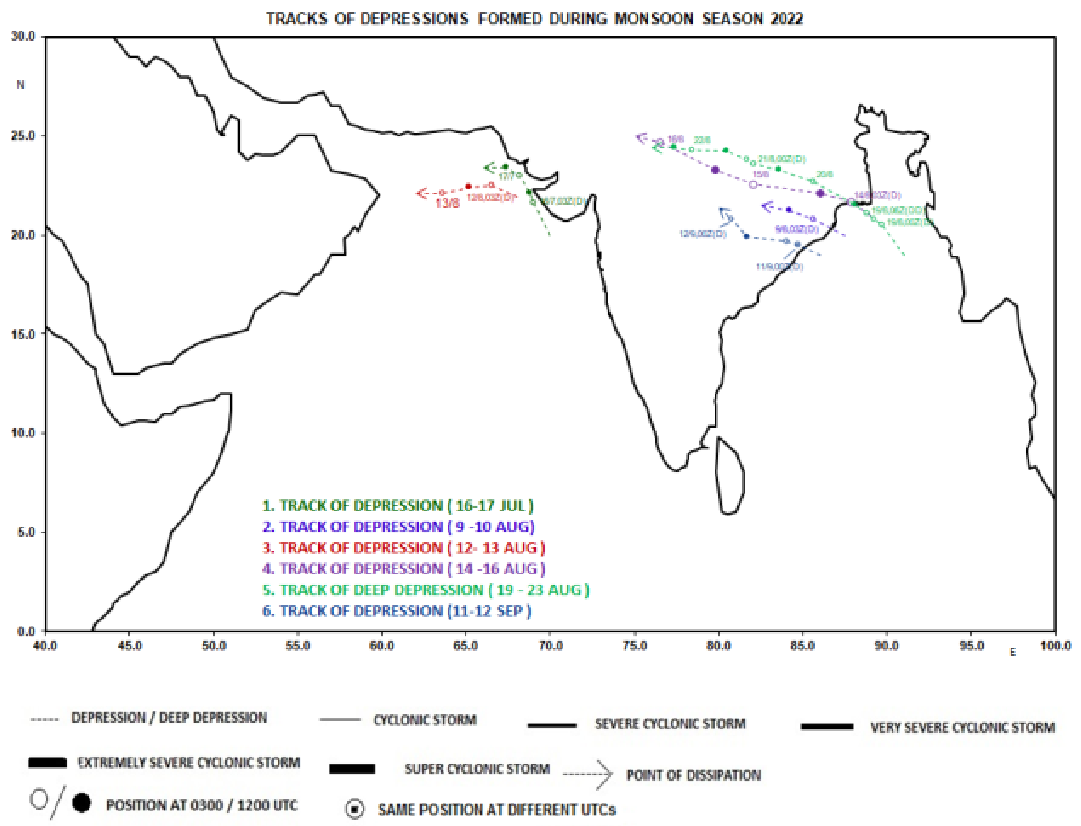
\includegraphics[width=1.1\linewidth, height=0.74\textheight]{images/IMD-report-2022.png}
%                     % 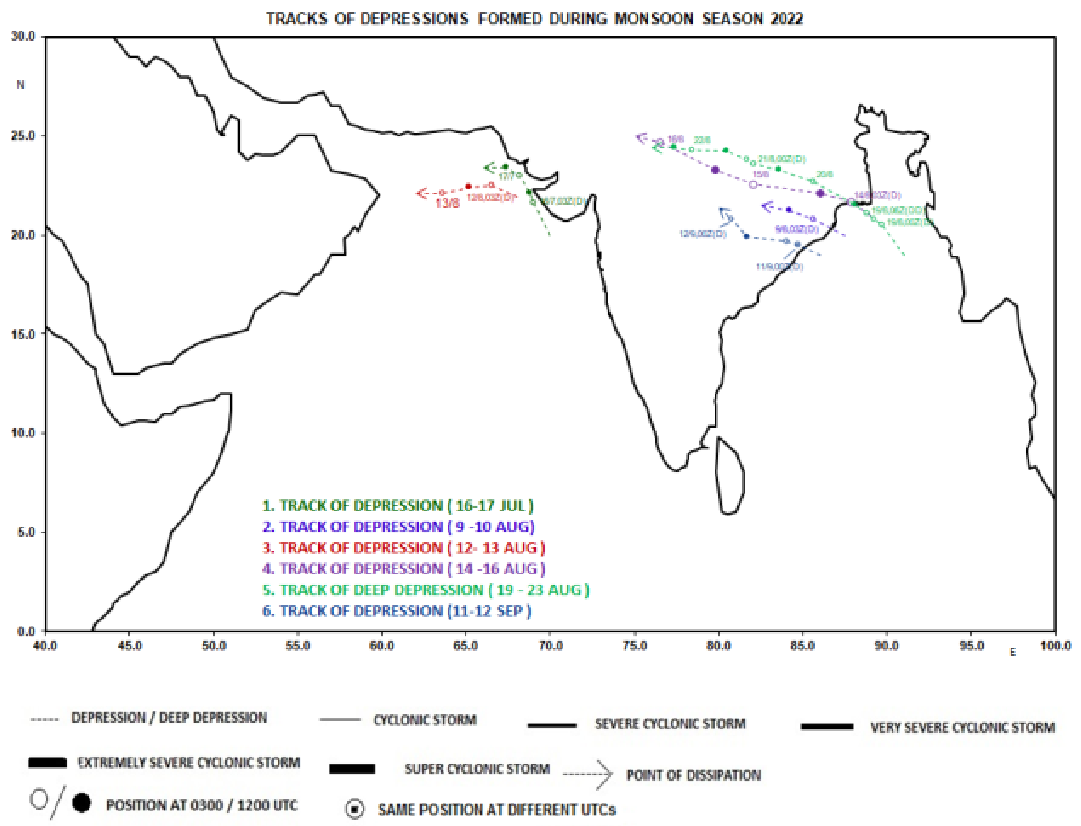
\includegraphics[width=1.12\linewidth, height=0.5\textheight, keepaspectratio]{images/IMD-report-2022.png}
%                 \end{figure}
%             \footnotesize IMD Annual Monsoon report 2022 \footnotemark[10]
%             \end{center}
%         \end{columns}
%
%         \vspace{-0.7cm}
%         \footnotetext[10]{\tiny Source : IMD Annual Monsoon Report 2022 (page 29) \href{https://mausam.imd.gov.in/imd\_latest/contents/ar2022.pdf}{\url{https://mausam.imd.gov.in/imd\_latest/contents/ar2022.pdf}}}
%     \end{center}
% \end{frame}

\subsubsection{Primitive MD detection for 2023}
\begin{frame}[label=tracks2023]{MD Tracks (June-September 2023)}
	\vspace{-0.5cm}
	\begin{center}
		\begin{columns}[T, onlytextwidth]
			\column{0.48\textwidth}
			\begin{center}
				\begin{figure}
					\includegraphics[width=1.1\linewidth]{../version15-with-no-ocean-masking/output_2023/MD_track_2023.png}
				\end{figure}
				\footnotesize Detected MD tracks using ERA5 single level Dataset (2023)
			\end{center}

			\vspace{-0.9cm}
			\column{0.48\textwidth}
			\begin{center}
				\begin{figure}
					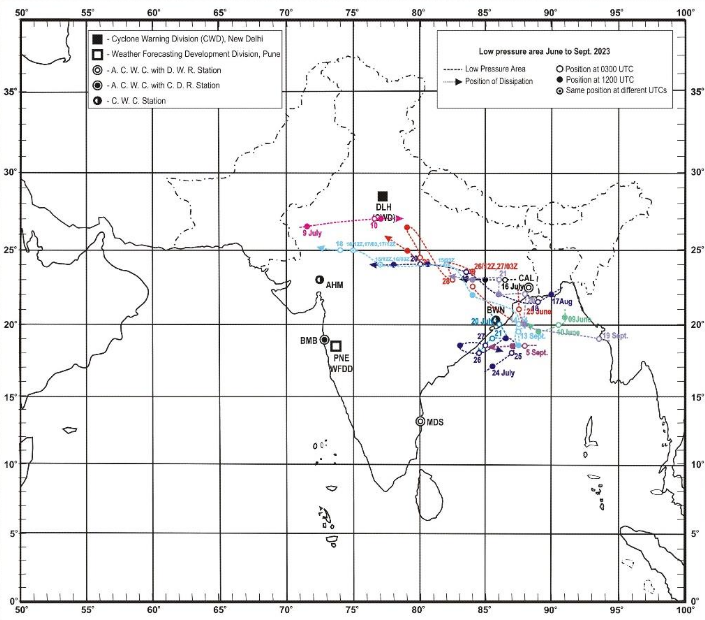
\includegraphics[width=1.1\linewidth, height=0.74\textheight]{images/IMD-report-2023.png}
					% 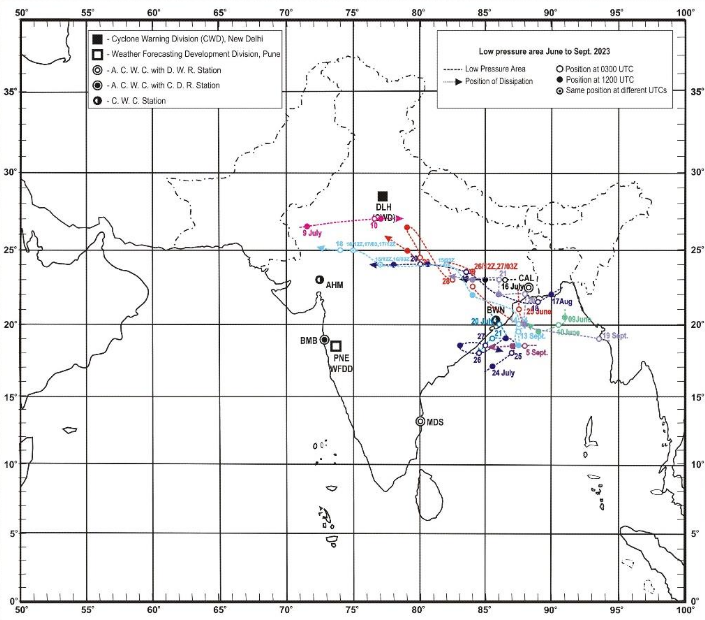
\includegraphics[width=1.12\linewidth, height=0.5\textheight, keepaspectratio]{images/IMD-report-2023.png}
				\end{figure}
				\footnotesize IMD Annual Monsoon report 2023 \footnotemark[10]
			\end{center}
		\end{columns}

		\vspace{-0.6cm}
		\footnotetext[10]{\tiny Source : IMD Annual Monsoon Report 2023 (page 23) \href{https://internal.imd.gov.in/press\_release/20231001\_pr\_2555.pdf}{\url{https://internal.imd.gov.in/press\_release/20231001\_pr\_2555.pdf}}}
	\end{center}
\end{frame}

\subsubsection{Primitive MD detection for 2025}
\begin{frame}[label=tracks2025]{MD Tracks (June-September 2025)}
	\vspace{-0.5cm}
	\begin{center}
		\begin{columns}[T, onlytextwidth]
			\column{0.48\textwidth}
			\begin{center}
				\begin{figure}
					\includegraphics[width=1.1\linewidth]{../version15-with-no-ocean-masking/output_2025/MD_track_2025.png}
				\end{figure}
				\footnotesize Detected MD tracks using ERA5 single level Dataset (2025)
			\end{center}

			\vspace{-0.9cm}
			\column{0.48\textwidth}
			\begin{center}
				\begin{figure}
					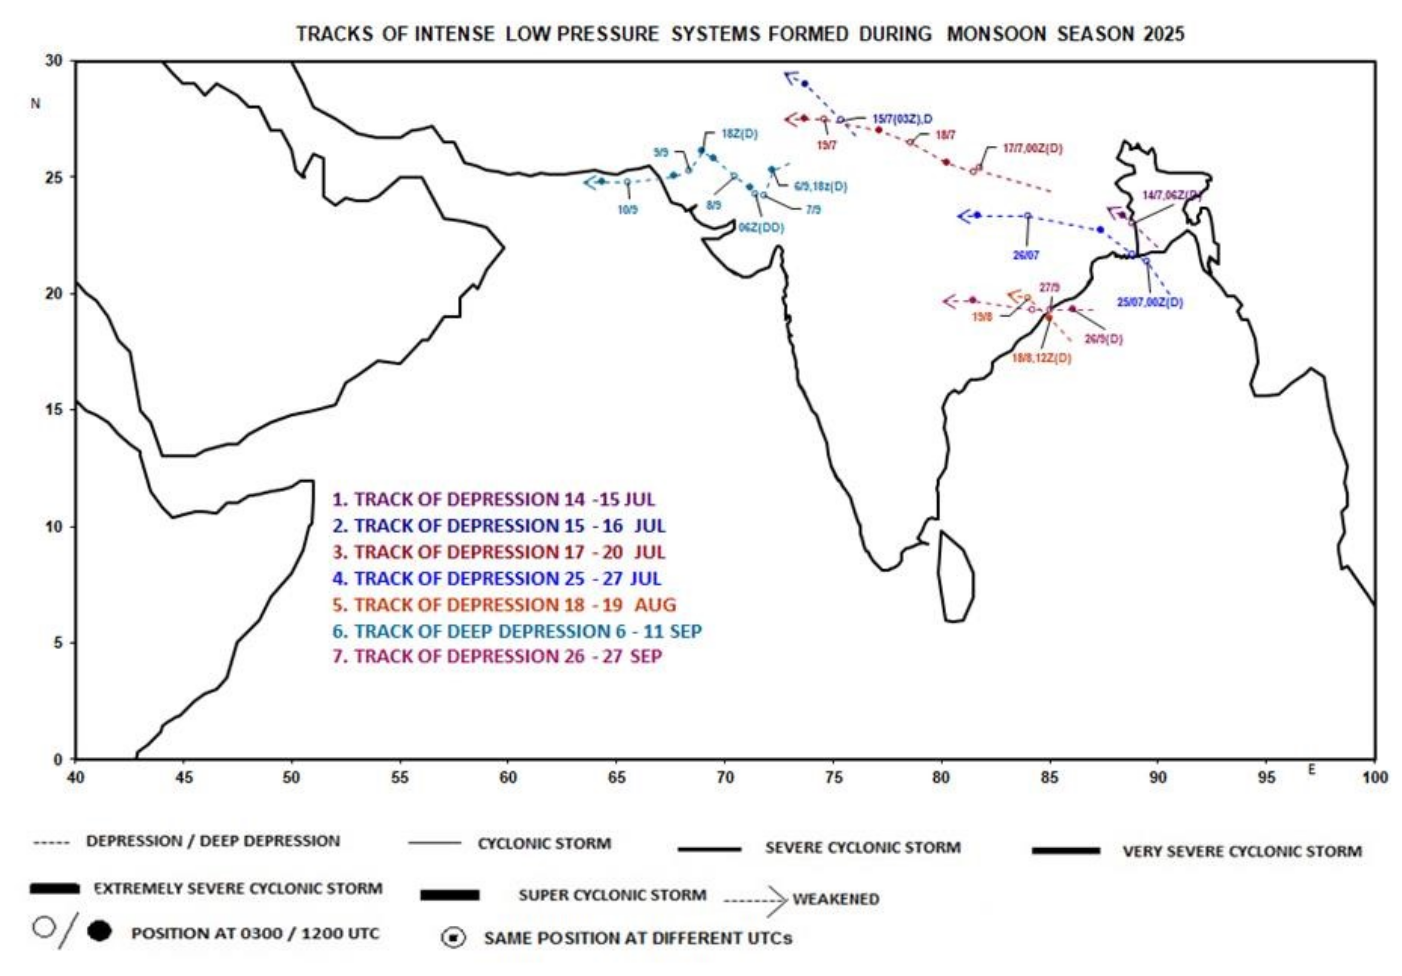
\includegraphics[width=1.1\linewidth, height=0.74\textheight]{images/IMD-report-2025.png}
					% 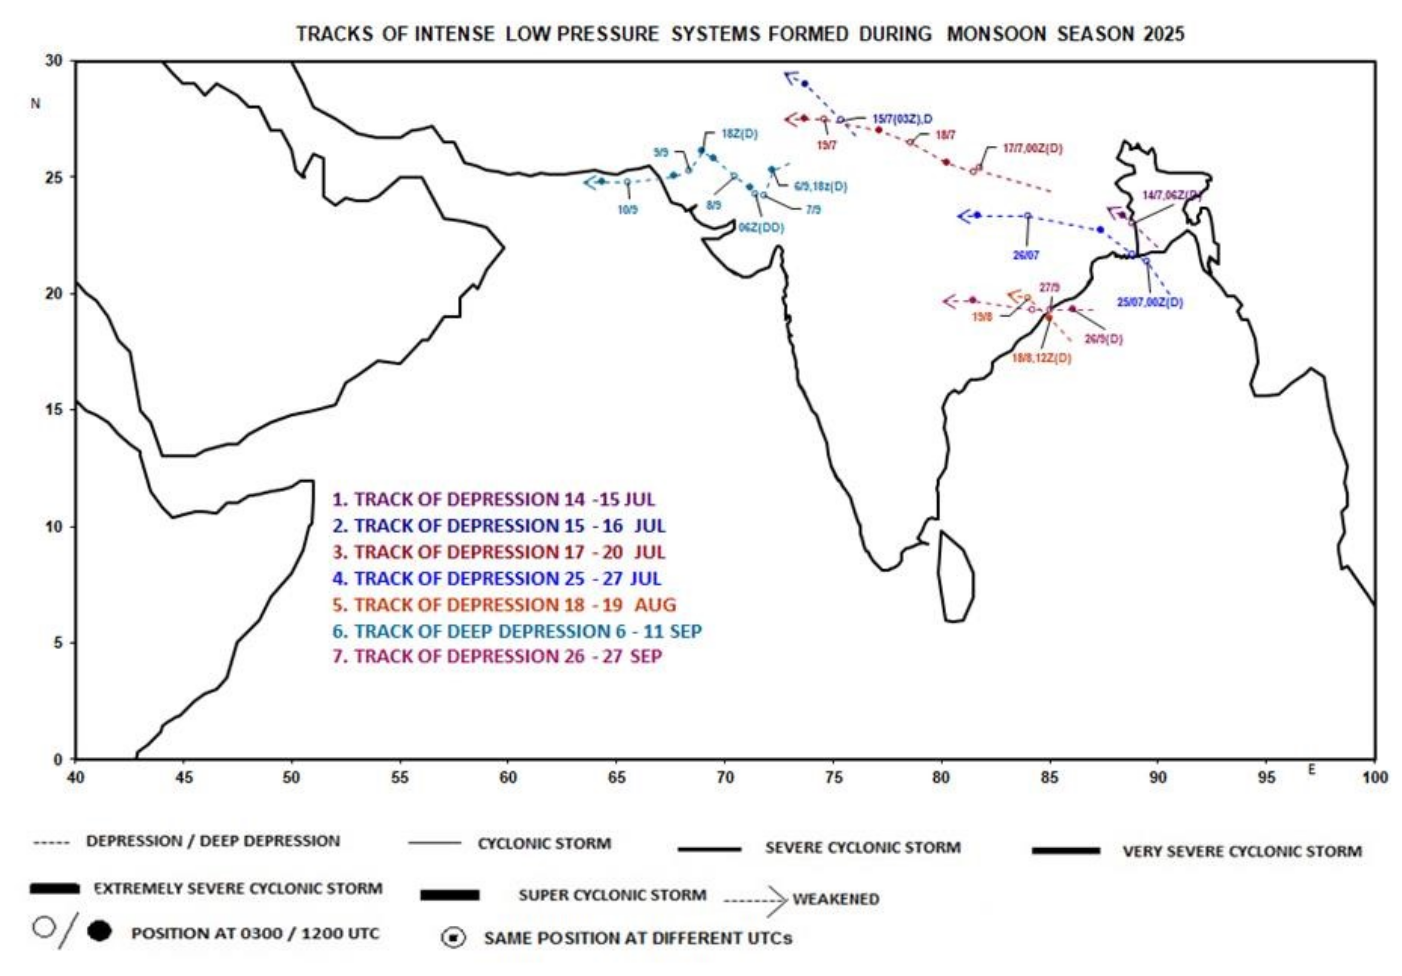
\includegraphics[width=1.12\linewidth, height=0.5\textheight, keepaspectratio]{images/IMD-report-2025.png}
				\end{figure}
				\footnotesize IMD Annual Monsoon report 2025 \footnotemark[10]
			\end{center}
		\end{columns}

		\vspace{-0.6cm}
		\footnotetext[10]{\tiny Source : IMD Annual Monsoon Report 2025 (page 7) \href{https://mausam.imd.gov.in/newdelhi/archive/2025-12-13/press\_release\_en.pdf}{\url{https://mausam.imd.gov.in/newdelhi/archive/2025-12-13/press\_release\_en.pdf}}}
	\end{center}
\end{frame}

\begin{frame}{Final Summary}
	\begin{center}
		\textbf{Why Some Monsoon Depressions Die Over Land While Others Survive?}

		\vspace{0.5cm}
		\textbf{Soil Moisture Determines Monsoon Depression Fate Over Land}

		\vspace{0.5cm}
		\footnotesize
		\begin{tabular}{lll}
			\toprule
			\textbf{Factor}                                                        & \textbf{Role}                       & \textbf{Timescale} \\
			\midrule
			Soil type sets the capacity, BUT elevation sets the infiltration rates & Days to weeks                                            \\
			Pre-landfall SM                                                        & Provides fuel (initial condition)   & Hours              \\
			Coupling strength                                                      & Sustains feedback (dynamic)         & Hours              \\
			Diurnal heating                                                        & Amplifies instability (daily cycle) & Hours              \\
			Memory                                                                 & Maintains persistence (multi-day)   & Days               \\
			\bottomrule
		\end{tabular}

		\vspace{0.3cm}
		\footnotesize
		\textit{All five factors work together. Missing any one limits longevity.}
	\end{center}

	\vspace{0.3cm}
	\textbf{Answer: Soil type and Pre-landfall condition matters as much as the atmosphere (Heat fluxes)}

	\vspace{0.3cm}
	\footnotesize
	\begin{itemize}
		\item Soil type sets the \textbf{capacity}.
		\item Elevation sets the \textbf{infiltration rates} (inversely proportional).
		\item Soil moisture sets the \textbf{fuel} for MD after Landfall weakening.
		\item Precipitation-soil feedback sets the \textbf{efficiency} also for longevity.
	\end{itemize}
\end{frame}


\section{References}
\begin{frame}[allowframebreaks]{References}
    \nocite{*}
    \scriptsize
    \printbibliography
\end{frame}
\end{document}
